% Created 2020-04-06 Mon 19:31
\documentclass[usenatbib]{mnras}
\usepackage[utf8]{inputenc}
\usepackage[T1]{fontenc}
\usepackage{graphicx}
\usepackage{grffile}
\usepackage{longtable}
\usepackage{wrapfig}
\usepackage{rotating}
\usepackage[normalem]{ulem}
\usepackage{amsmath}
\usepackage{textcomp}
\usepackage{amssymb}
\usepackage{capt-of}
\usepackage{hyperref}
\usepackage{natbib}
\usepackage{pgfplots}
\usepgfplotslibrary{groupplots,dateplot}
\usetikzlibrary{patterns,shapes.arrows}
\pgfplotsset{compat=newest}
\usepackage{dsfont}
\author{Aleksandr Petrosyan, William J. Handley}
\date{\today}
\title{Cosmological parameter estimation using Bayesian accelerated machine learning}
\hypersetup{
 pdfauthor={Aleksandr Petrosyan, William J. Handley},
 pdftitle={Cosmological parameter estimation using Bayesian accelerated machine learning},
 pdfkeywords={},
 pdfsubject={},
 pdfcreator={Emacs 26.3 (Org mode 9.1.9)}, 
 pdflang={English}}
\begin{document}

\maketitle
\begin{abstract}
TODO
\end{abstract}

\section{Introduction}
\label{sec:org5d61c95}

The standard model of the universe and its evolution in modern
cosmology is the accepted \(\Lambda\)CDM model \citep{Condon2018},
so named after the main components of the universe according to
it. It has six major parameters: physical baryon density parameter;
physical dark matter density parameter; the age of the universe;
scalar spectral index; curvature fluctuation amplitude; and
re-ionization optical depth. It is the task of the present study to
evaluate how well does \(\Lambda\)CDM agree with observations from
the Planck mission \citep{planck}, as well as provide estimates for
the main parameters. It is also our goal to find methods for
accelerating said process. In this section we shall describe the
main approaches one may take to answering these questions, as well
as refinements made to them.

The problem of reconciling theoretical predictions with experimental
observations is the fundamental underpinning of any modern science,
be it Physics, or Biology. The methods and the general statistical
frameworks used for such reconciliation have changed almost as much
as the sciences themselves. Indeed, while a simple qualitative ``all
objects in vacuo accelerate at a rate independent of their mass'',
may have been sufficient for Galileo, modern problems necessitate
modern solutions. Although the slightly more informative ``the
acceleration of free fall was measured \(g = 9.81 \pm 0.01\) is an
improvement, it leaves much to be desired. For example, we
implicitly assume that the distribution of \(g\) is symmetrical
around \(\left \langle g \right \rangle = 9.81\). This may not be
the case if we're using free fall to measure \(g\), as almost every
source of error: slow reaction times, air drag, inconsistent
release; would lead to an underestimate of \(g\). 

To establish a law of physics, one needs finer tools and more
precise language to make all of the implicit assumptions explicit,
so one can judge whether or not the conclusions are justified given
the observations.

Enter Bayesian inference. It is based on the mathematical result
obtained by \cite{1763}, and was refined over the following two
centuries. This approach has proven quite fruitful in computational
problems \citep{Wolpert2004}, particularly in Machine learning, and is
slowly making its way into physics, a field traditionally dominated
by frequentist statistics. Without going into too much detail for
the reasons behind Bayesian probability's success, we should point
out that it is able to reproduce the results of traditional
inference techniques, while putting them into a more general
framework, making the delineations of objectivity and subjectivity
explicit.


By performing a full Bayesian analysis one can find quantitative
answers to questions that otherwise could only be answered
qualitatively.  For example: how consistent a model is with our
observations is quantified in \emph{evidence}. How liable are each
individual values of the model parameters is quantified in the
\emph{posterior}. Moreover, there exists a mathematical object
representing  the vast body of experience we  have accrued from
other observations -- the \emph{prior}. 

Some aspects of a model may be for various reasons more interesting
than others. One may like to build a model that describes a
free-falling object in an evacuated tube, but be mainly concerned
with the gravitational aspects of the process. Bayesian worldview
allows one to \emph{marginalise} the model parameters that one does not
care about: so-called \emph{nuisance} parameters. Mathematically this is
represented by conditional probabilities, and as the name suggests,
the cornerstone of the mathematics of such objects is Bayes'
theorem. 

The above advantages make Bayesian inference a particularly
convenient methodology for estimating cosmological
parameters. Although \$\(\Lambda\)\$CDM has few parameters, the accurate
model describing the physical processes that Planck \citep{planck}
observed needs at least 27 parameters, not counting the calibration
parameters for the experimental apparatus, and other, more
complicated models, which lead to models with 42 parameters.

A full Bayesian inference for such a large parameter space is a
computationally expensive endeavour, particularly very little prior
knowledge. Hence a large number of algorithms were developed to
accelerate the computation: Metropolis-Hastings \citep{Metropolis}
used in conjunction with the Gibbs sampler
\citep{Metropolis-hastings-gibbs}, Hybrid (Hamiltonian) Monte-Carlo
\citep{1701.02434,Duane_1987} and more recently Nested Sampling
\citep{skilling2006}, which will be our focus.

Nested Sampling, as described by \citeauthor{skilling2006} is rather
abstract, and multiple algorithmic-ally distinct implementations of
the idea exist including:
\begin{itemize}
\item MultiNest \citep{Feroz2009MultiNestAE},
\item nestle \citep{nestle}
\item dyNesty \citep{Speagle_2020},
\item PolyChord \citep{polychord}.
\end{itemize}
Although the optimisation proposed in this paper is quite general,
in that it accelerates all implementations of nested sampling, we
shall primarily focus on PolyChord. Among the many reasons, is that
the slice sampling algorithm used in PolyChord, is the one that is
most liable to be adversely affected by the stochastic nature of the
re-partitioning proposed here.

\cite{chen-ferroz-hobson} noted that the nested sampling algorithm,
unlike other Markov-chain Monte-Carlo algorithms, is sensitive to
how the two conditional probabilities \emph{likelihood} and \emph{prior} are
defined, with respect to the posterior distribution. Hence the name
of the technique -- \emph{automatic power posterior re-partitioning}
(PPR). While \citeauthor{chen-ferroz-hobson} used PPR to improve the
stability of convergence for prior distributions that may have been
at variance with the true posterior, we shall show that it can be
used to accelerate the execution of the nested sampling
algorithm. 

The purpose of this paper is to present a mathematical framework
that encapsulates the idea and explores the extents of its
utility. In particular, we shall describe how one may achieve better
convergence stability and better performance, using mixture
re-partitioning, a technique that we've devised specifically for
improving the performance of nested samplers.

In the following sections we shall (mostly) focus on the theoretical
background, and an extension (more precisely generalisation) of the
idea of posterior re-partitioning, its advantages, applicability and
how it can be used to improve run-time characteristics of samplers
such as PolyChord. Lastly we shall present the results of using such
methods when applied to a modern Cosmological parameter estimator
such as Cobaya \citep{cobaya}.

\section{Background theory}
\label{sec:org7b529cf}

\subsection{Brief primer on Bayesian inference.}
\label{sec:org8861d37}

This topic has been discussed at length in literature
\citep{jeffreys2010scientific}, so we shall restrict ourselves to the
bare necessary definitions and concepts.

Let a scientific theory that we're interested in testing, provide a
model of a process model \({\cal M}\), that predicts what data \(\lbrace {\cal M}(\vec{\theta})\rbrace\) one observes, based on the
parameters \(\vec{\theta} = \lbrace \theta_1, \theta_2, \ldots,
   \theta_n \rbrace\) (we shall drop the vector, the nature of
\(\theta\), should be obvious from the context) and the (actual)
observed data -- \(D\).

One can define the following conditional probabilities given
in \autoref{table-defs}. Using these definition \citeauthor{1763} 's theorem
becomes
\begin{equation}
 {\cal L} \pi (\theta) = {\cal Z} {\cal P} (\theta).
\label{eq:bayes} 
\end{equation}
Notice that the \emph{evidence} \({\cal Z}\) is implicitly defined as

\begin{equation}\label{eq:def-z}
 {\cal Z} = \int_{\Psi} {\cal L}(\theta) \pi(\theta) d\theta, 
\end{equation}
where \(\Psi\) is the so-called prior space -- the domain of the
prior function. Although some authors
(e.g. \citeauthor{jeffreys2010scientific}) believe \({\cal Z}\) to be
no more than a normalisation factor, as one can see from its
definition in \autoref{table-defs}, it quantifies the consistency of
the hypothesised model with the observed data. Therefore, it's a
suitable measure of the ``goodness'' of a model: the higher the
value of \({\cal Z}\), the more likely is that the model accurately
describes the physical process in question.

\begin{table}[htbp]
\caption{Definitions of main quantities in Bayesian analysis. \label{table-defs}}
\centering
\begin{tabular}{lll}
\textbf{\textbf{Term}} & \textbf{\textbf{Symbol}} & \textbf{\textbf{Definition}}\\
\hline
Prior & \(\pi(\theta)\) & \(P ( \theta  \vert D)\)\\
Likelihood & \({\cal L}(\theta)\) & \(P ( D \vert \theta \cup M)\)\\
Posterior & \({\cal P}(\theta)\) & \(P ( \theta \vert D \cup M)\)\\
Evidence & \({\cal Z}\) & \(P ( D \vert M)\)\\
\end{tabular}
\end{table}

The two independent quantities, \({\cal L}\) and \(\pi\) defined in \autoref{table-defs} are the
inputs to the Bayesian Sampler. How they are specified depends on the algorithm, however, most nested samplers (e.g. PolyChord) find a convenient representation of log-likelihood: 
\begin{equation}
  L = \ln \cal L
\end{equation}
and the \emph{prior quantile} function, also referred to as the \emph{inverse
cumulative distribution function} (iCDF) for the prior distribution.
\begin{equation}
 \pi : HC \rightarrow \Psi,
\end{equation}
that is, a mapping from a unit hypercube where the distribution of
parameter images is uniform, onto the (non-uniform) prior space
that is the domain of integration of \({\cal Z}\). Choosing to work
with logarithms is a convenience: most likelihoods are Gaussian
(central limit theorem \cite{central-limit-theorem}), hence taking
the logarithm early allows us to avoid costly numerical
multiplications and divisions in lieu of additions and
subtractions. The reason for working with the quantile as opposed
to the probability density function (PDF) or the cumulative
distribution function (CDF) shall become clear later.

An important point is that within specification of likelihood and
prior there is some redundancy. One can easily see that by
considering another pair of input functions such that 
\begin{equation}
  \tilde{\cal L} \tilde{\pi} = \cal L \pi. 
\end{equation}
In the new representation, the value of \({\cal Z}\) is invariant
and by \autoref{eq:bayes}, so is \({\cal P}(\theta)\).  

Thus, most MC-MC Bayesian samplers are indifferent to precise
definitions of \(\cal L\) and \(\pi\), as long as their product --
the posterior, corresponds to an element of physical reality. One
notable exception and therefore of interest to us is nested
sampling.

\subsection{Nested Sampling.}
\label{sec:org836af1b}

This algorithm is discussed in depth, so we shall restrict
ourselves to descriptions that are necessary for understanding how
and why posterior re-partitioning works.

We shall begin by noting that, Bayes' theorem reduces the problem
of parameter estimation to integration, so hypothetically the naive
approach would be to rasterise the prior space \(\Psi\) and
numerically evaluate the integral \({\cal P}\). However, in
hypotheses with many parameters, said problem is intractable by
uniform rasterisation (i.e. using a grid and enumerating all the
points), thus Monte-Carlo techniques are favoured.

For simplicity and without loss of generality assume that the prior
space is a unit hypercube. Draw, at random, \(n_\text{live}\)
points from the hypercube. One expects that the probability that
two points have the same likelihood is vanishing, so each of them
lies on a distinct iso-likelihood hyper-surface. Each will contain
on-average \(frac{1}{n_\text{live}}\)-th of the total volume of the
hypercube. More specifically, each shell's volume shall have some
deviation \(\Delta\), from said value, with an associated probability
distribution \(P(\Delta)\).

Subsequently, we may wish to pick another point at random, but
requiring that the likelihood of that point is higher than the
lowest likelihood of the initial choice, we can ``move'' the
outermost point inside. In \citeauthor{skilling2006} 's notation, the
aforementioned point with the lowest likelihood becomes ``dead''
and the new point becomes ``alive''. Moreover, our argument for
hyper-surfaces encasing a roughly equal volume still holds, so we
can expect that upon next iteration the prior volume encased in the
outermost hyper-surface is reduced by
\(\frac{1}{n_\text{live}}\)-th of the volume encased in the
previous outer-most shell.

More formally, this defines a sequence of approximations of the
prior volume encased in the outer hyper-surface:

\begin{equation}
  \begin{array}{rcl}
  X_{0} &=  &1 \\
  X_{1} &= &X_{0} \left(1- \frac{1}{n_\text{live}}\right)\\
  & \vdots & \\
  X_{i} &= &X_{i-1}\left(1- \frac{1}{n_\text{live}}\right)\\
  & \vdots &
\end{array}
\label{eq:recurrence-relation}
\end{equation}

which allows us to iteratively pick ``live'' points closer to
regions where the likelihood is high. A suitable termination
criterion therefrom is to stop when the prior volume encased in the
shell is lower than a predetermined fraction of the total hypercube
volume -- \(1\).

As was mentioned previously, the recurrence relation
\eqref{eq:recurrence-relation} is not exact. However, \(P(\Delta)\)
is a known distribution, dependent on the dimensionality of the
hypercube and the likelihood. Thus, one can for each value of
\(\epsilon>0\), deduce a value \(\delta(\epsilon) >0\), such that
\(P(\Delta > \delta) < \epsilon\). Hence, by choosing \(\epsilon\)
based on \(n_\text{live}\), one gets a characteristic value for the
error \(\delta\). Carrying these through the iterations allows us to
estimate the prior volume and hence the evidence up to some
precision.

This algorithm can be generalised to other priors and prior spaces
by virtue of coordinate transformations, which are represented by
iCDFs.

The algorithm's run-time is linearly dependent on
\(n_{live}\). However, in context of cosmological parameter
estimation, the more important number is the quantity of likelihood
evaluations, as the function \({\cal L}\) is the dominant cost; for
example, In Cobaya using the CLASS provided likelihood function one
evaluation can take upwards of a second. 

Naturally, under such circumstances, algorithms that minimise the
number of likelihood evaluations will offer the most
improvement. For example, rejection sampling: drawing a point at
random, and rejecting it based on the criteria mentioned, is less
efficient than slice sampling \citep{Neal_2003}.

So when does one terminate the fastest? One suspects that knowing
the posterior distribution, all the algorithm needs to do is check
the obtained values. So an ideal sampler would converge optimally
when the prior and the posterior coincide: 
\[\begin{array}{rl} {\cal P}(\theta) = \pi(\theta) & \forall \theta \end{array} \]
So if one has gathered data from free fall experiments, on earth
one would expect the posterior to be a normal distribution peaked
at \(g=9.81\), with standard deviation \(\sigma_{g} = 0.01\), which we
shall compactly refer to as \[{\cal P}(\theta) = G(9.81, 0.01)\].

However that is only partially true. According to Bayesian
statistics the prior knowledge: the constraints set on the model
parameters, are pare thereof, so by picking a different,
\emph{unrepresentative prior} the likelihoods will not correspond to the
same model. 

In our particular example, if the free-fall data was gathered on
the surface of the moon, and we use the earth prior for \(g\),
nested sampling would converge on a Gaussian peaked at \(g=9.81\),
with perhaps a broader standard deviation. Evidence would be the
main telltale sign that the algorithm has not produced a
statistically significant or meaningful result, but that too can be
masked by other parameters. Indeed, if one has set a gnerous
uniform prior on the air-drag coefficient, and admitted the
detector spacing as well as trigger timing to be nuisance
parameters, one will not see anomalies\footnote{this peculiarity of
statistical methods lead John Von Neumann to remark that four
parameters in a model were sufficient to produce a statistically
significant fit to an elephant. And that five would be consistent
with it moving its trunk.}.

This is the problem of \emph{unrepresentative priors} and
\citeauthor*{chen-ferroz-hobson} have developed power-posterior
repartitioning specifically as a mitigation of the aforementioned
issue.


\subsection{Power posterior re-partitioning}
\label{sec:org7ae6d1f}

The basic idea is as follows. If we had two priors, one much
narrower than the other, we expect that the convergence in the
narrower one will be faster. After all, we're ignoring the bulk of
prior space where nothing happens. We also expect that the
likelihood of the values inside the smaller effective volume will
be enhanced. To see why this happens, consider that to have a
larger value of the prior, (or rather a more condensed one), in
order to keep the product \(\cal L \pi\) constant, one must have
reduced the value of \(\cal L\), conversely, if the value is not
reduced, it is larger than it would have been.


As such, \citeauthor{chen-ferroz-hobson} have proposed introducing an
extra parameter \(\beta\) that re-scales the prior:
\begin{equation}
  \tilde{\pi}(\theta) = \frac{\pi(\theta)^{\beta}}{Z(\beta)\{\pi\}},
\end{equation}
where \(Z(\beta)\{\pi\}\) is a normalisation factor, i.e. 
\begin{equation}
  Z(\beta)\{\pi\} = \int_{\theta \in \Psi} \pi(\theta)^{\beta}d\theta.
\end{equation}
According to their prescription, one also needs to modify the likelihood
\begin{equation}
  \tilde{\cal L}(\theta) = {\cal L}(\theta) Z(\beta)\{\pi\} \cdot \pi^{1-\beta}(\theta).
\end{equation}
One needs to take great care when choosing the domain of
\(\beta\). As \(\beta\) is an ordinary nuisance parameter it needs a
prior, and one has very few restrictions. Normally we expect a
uniform prior \(\beta \in [0, 1]\). If one is confident that the
original prior was representative one could introduce a non-linear
map that favours the value \(\beta=1\). If the original prior may be
too broad one could experiment and extend \(\beta>1\). One can also
extend it to \(\beta<0\), although practical cases where that may be
a sensible option are few.

Notice, however, that \citeauthor{chen-ferroz-hobson}, our argument
implicitly assumed that the prior we started with was
peaked. Indeed the sole difference between different values of
\(\beta\), for a uniform prior would be the normalisation, which by
construction we constrain to the original value.


Importantly the domains of all functions need to be the same. Let
\(D(f)\) denote the domain of the function \(f\), i.e. where the
function is both defined and \textbf{non-zero}. Hence
\begin{equation}
  D(\pi) = D({\cal L}) = \Psi = D({\cal P}),
\end{equation} 
meaning the posterior is within the domain of the prior and
likelihood, which will be important later.\label{domain-discussion}

This, for the cases that \citeauthor{chen-ferroz-hobson} have
originally considered, resolves the issue of non-representative
priors, because the evidence associated with the biased prior
reduces as \(\beta\rightarrow0\).

In the original form, this method is to prevent errors, by
sacrificing run-time performance. In practice, the overhead
associated with PPR is negligible, and even in the case of
univariate examples, where the relative impact is maximal, it's not
significant \cite[see numerical
examples]{chen-ferroz-hobson}. Even so, it can only do that under the assumption that
one's prior knowledge is not represented by a uniform distribution. 

Our first discovery pertains to what happens under an inverted
premise: can one gain performance by starting with a uniform prior,
and using PPR backwards to accelerate convergence?

Let us have a model, of which prior experience is ignorant. Under
such circumstances the prior is uniform (and unbounded, which we
shall ignore for now). Central limit theorem suggests, that the
model parameters' posterior is within a Gaussian:
\begin{equation}
 \pi (\theta) \propto \exp \left[-\left(\frac{\theta - \mu}{2\sigma}\right)^{2} \right],
\end{equation}
albeit not the values of \(\mu\) and \(\sigma\). We shall refer to
this function as the \emph{intuition}, or the \emph{biased prior}. Ordinarily
this intuition is subjective, and therefore can affect the
objectivity of our outcomes. However, with a proper methodology one
can have the best of both worlds: the performance associated with
knowing the result in advance, with the flexibility to entertain
other possible results.

One can achieve these results using PPR. Consider what happens on
the microscopic level, A point with fully random coordinates is
drawn from an \(n+1\) dimensional space where the effective
parameter vector contains \(\beta\) as the last parameter, treated
as any other component of \(\theta\). This randomises the prior, live
points that are closer to the true posterior distribution are
favoured, so are values of \(\beta\) which lead to points with
higher likelihood.  This feedback ensures that if the true
posterior is within the region of radius \(\sigma / \beta\) of the
chosen value of \(\mu\), then the new points are chosen
preferentially from that region. The re-normalisation of the
likelihood, ensures that the posterior distribution is not biased
towards the value of \(\mu\), but rather the true posterior; one
that we would have found had we used a uniform prior. If our
hypothesis was wrong, then the values of \(\beta \rightarrow 0\)
would be favoured. The effective prior would then tend to a uniform
distribution.

\begin{figure}\label{fig:ppr}
 \input{./illustrations/ppr.tex}
\caption{A demonstration of the function \(\tilde{\pi}(\theta; \beta)\) for different values of \(\beta\). Note that we've started under the assumption that the distribution is a truncated Gaussian, i.e. that it is zero outside the range \((-1, 1)\). This manifests as sharp changes in curvature at the boundaries. Note that \(\forall \beta\), \(\int_{-1}^{1}\tilde{\pi}(\theta; \beta) = 1\).}
\end{figure}

Having demonstrated correctness, let's focus on performance. The
majority of the run-time of nested sampling with a uniform prior is
spent ``compressing'' the live points onto the posterior
distribution. With \(\beta>0\), the probability that points will be
chosen from high-likelihood regions is enhanced, so on average the
execution time should decrease. 


\subsection{Argument scaling}
\label{sec:org76848ff}

Power posterior re-partitioning in the case of a Gaussian
distribution (also a Cauchy distribution), can be thought of as
scaling the distribution using \(\beta\).

We shall discuss multiple forms, of such re-partitioning schemes,
and extend the idea to discontinuous distributions, such as a
re-sizeable uniform prior.  

So far, the main practical considerations for choosing such a
distribution is that for some attainable value of \(\beta\), the
distribution resolves to a reference. For that reason, for example
the Cauchy distribution is also more convenient to treat using a
power, because the manifest reduction to a uniform distribution is
obvious when raising the entire distribution to the power of
\(\beta\), and not when it pre-multiplies the breadth parameter
\(\gamma\).

A drawback of using power re-partitioning is that it's not always
possible to find an analytical result for \(Z(\beta)\{\pi\}\), indeed
in the case of trigonometric distributions, such \(Z(\beta)\{\pi\}\),
was proven to only be analytical if \(\beta\), is an integer, and
proven not to be analytical otherwise \citep{Liouville1837}. Mixture
re-partitioning on the other hand can easily cope with such
functions, as it only requires for them to be normalised once
(e.g. for \(\beta=0\) and \(\beta=1\)), and re-use the normalisation
factor.

\subsection{General automatic posterior re-partitioning.}
\label{sec:orgb1b639e}

Let's recap the key components of posterior re-partitioning. We have
   a baseline prior, with its likelihood \((\pi(\theta), \cal L
      (\theta))\), and a parameterised pair of biased prior and
   likelihood \((\pi'(\theta; \beta), \cal L' (\theta;
      \beta))\). These need to satisfy the following requirements.

\begin{enumerate}
\item For some \(\beta_{0}\), \(\pi'(\theta; \beta) \equiv \pi(\theta)\)
similarly \({\cal L'(\theta, \beta) \equiv {\cal L}}\). This is
the \textbf{\textbf{specialisation property}}.\label{spec-prop}
\item The product of the parameterised pair is constant for all values
of \(\beta\) and by specialisation property : \(\pi'(\theta; \beta)
      \cal L' (\theta; \beta) = \pi(\theta), \cal L (\theta)\). This is
the \textbf{\textbf{normalisation property}}.\label{norm-prop}
\item We need there to be a guiding dynamical principle that favours
the representative prior, i.e. one that's closest to the
posterior distribution, which we call the \textbf{\textbf{convergence
property}}.\label{conv-prop}
\end{enumerate}

PPR satisfies all three properties as follows: \ref{spec-prop} is
fulfilled with defining \(\pi'(\theta; 0) =
   \pi(\theta)\). \ref{norm-prop} is fulfilled by construction and
\ref{conv-prop},  by noting that \(\lim_{\beta
   \rightarrow 0} \pi'(\theta; \beta) = \pi(\theta)\).

Whether, the extra complexity is offset by the speedup offered by
the correct bias, depends on both how accurate our bias is, and on
the dimensions of the problem. In most cases the complexity of the
likelihood calculation is negligible, as well as the extra
dimension.

Any functions that satisfy the above requirements should produce
the same result, and our goal is to identify which shall produce
better run-times.

\subsubsection{Additive mixtures.}
\label{sec:org560e8ca}
Consider a weighted sum of a uniform distribution with
a Gaussian, e.g. in one dimension
\begin{equation}\label{eq:additive-mix}
  \pi(\theta) = \dfrac{ \left\lbrace \frac{1- \beta} {b - a} + \beta \exp \left[ -\left(\frac{\theta - \mu}{\sigma} \right)^{2}\right]\right\rbrace \cdot TH(\theta; a, b)}{Z}.
\end{equation}
where \(TH(\theta;a,b)\) is the top-hat function. Integrate to
obtain the normalisation factor \(Z(\beta)\{\pi\}\), used to
re-scale \({\cal L}\). Recall, however, that we use the inverse of
the prior cumulative distribution, and while the inverses of both
priors are manifest, we cannot easily compute the inverse of the
sum. In general one can't even prove that for two arbitrary
distributions the inverse of the sum exists.

\begin{figure}
  % This file was created by tikzplotlib v0.9.1.
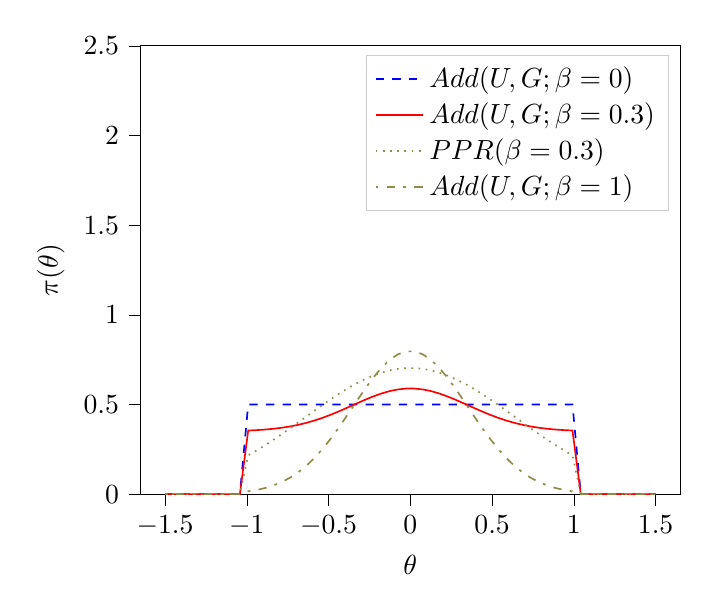
\begin{tikzpicture}

\begin{axis}[
legend cell align={left},
legend style={fill opacity=0.8, draw opacity=1, text opacity=1, draw=white!80!black},
tick align=outside,
tick pos=left,
x grid style={white!69.0196078431373!black},
xlabel={\(\displaystyle \theta\)},
xmin=-1.65, xmax=1.65,
xtick style={color=black},
y grid style={white!69.0196078431373!black},
ylabel={\(\displaystyle \pi(\theta)\)},
ymin=0, ymax=2.5,
ytick style={color=black}
]
\addplot [semithick, blue, dashed]
table {%
-1.5 0
-1.44915254237288 0
-1.39830508474576 0
-1.34745762711864 0
-1.29661016949153 0
-1.24576271186441 0
-1.19491525423729 0
-1.14406779661017 0
-1.09322033898305 0
-1.04237288135593 0
-0.991525423728814 0.5
-0.940677966101695 0.5
-0.889830508474576 0.5
-0.838983050847458 0.5
-0.788135593220339 0.5
-0.73728813559322 0.5
-0.686440677966102 0.5
-0.635593220338983 0.5
-0.584745762711864 0.5
-0.533898305084746 0.5
-0.483050847457627 0.5
-0.432203389830508 0.5
-0.38135593220339 0.5
-0.330508474576271 0.5
-0.279661016949152 0.5
-0.228813559322034 0.5
-0.177966101694915 0.5
-0.127118644067796 0.5
-0.0762711864406778 0.5
-0.0254237288135593 0.5
0.0254237288135595 0.5
0.076271186440678 0.5
0.127118644067797 0.5
0.177966101694915 0.5
0.228813559322034 0.5
0.279661016949153 0.5
0.330508474576271 0.5
0.38135593220339 0.5
0.432203389830509 0.5
0.483050847457627 0.5
0.533898305084746 0.5
0.584745762711865 0.5
0.635593220338983 0.5
0.686440677966102 0.5
0.737288135593221 0.5
0.788135593220339 0.5
0.838983050847458 0.5
0.889830508474577 0.5
0.940677966101695 0.5
0.991525423728814 0.5
1.04237288135593 0
1.09322033898305 0
1.14406779661017 0
1.19491525423729 0
1.24576271186441 0
1.29661016949153 0
1.34745762711864 0
1.39830508474576 0
1.44915254237288 0
1.5 0
};
\addlegendentry{$Add(U, G; \beta=0)$}
\addplot [semithick, red]
table {%
-1.5 0
-1.44915254237288 0
-1.39830508474576 0
-1.34745762711864 0
-1.29661016949153 0
-1.24576271186441 0
-1.19491525423729 0
-1.14406779661017 0
-1.09322033898305 0
-1.04237288135593 0
-0.991525423728814 0.354690318349014
-0.940677966101695 0.356948257984
-0.889830508474576 0.360082465104504
-0.838983050847458 0.364330940676924
-0.788135593220339 0.369952616124693
-0.73728813559322 0.377210854126332
-0.686440677966102 0.386349771016284
-0.635593220338983 0.397563999166328
-0.584745762711864 0.410963827347145
-0.533898305084746 0.426539084688447
-0.483050847457627 0.444126407270881
-0.432203389830508 0.463385332657938
-0.38135593220339 0.483788705911657
-0.330508474576271 0.504631940380111
-0.279661016949152 0.525063713430144
-0.228813559322034 0.54413786330865
-0.177966101694915 0.560882981292239
-0.127118644067796 0.574383024711279
-0.0762711864406778 0.583859836479305
-0.0254237288135593 0.588747297055759
0.0254237288135595 0.588747297055759
0.076271186440678 0.583859836479305
0.127118644067797 0.574383024711279
0.177966101694915 0.560882981292239
0.228813559322034 0.54413786330865
0.279661016949153 0.525063713430144
0.330508474576271 0.504631940380111
0.38135593220339 0.483788705911657
0.432203389830509 0.463385332657938
0.483050847457627 0.444126407270881
0.533898305084746 0.426539084688447
0.584745762711865 0.410963827347145
0.635593220338983 0.397563999166328
0.686440677966102 0.386349771016284
0.737288135593221 0.377210854126332
0.788135593220339 0.369952616124693
0.838983050847458 0.364330940676924
0.889830508474577 0.360082465104504
0.940677966101695 0.356948257984
0.991525423728814 0.354690318349014
1.04237288135593 0
1.09322033898305 0
1.14406779661017 0
1.19491525423729 0
1.24576271186441 0
1.29661016949153 0
1.34745762711864 0
1.39830508474576 0
1.44915254237288 0
1.5 0
};
\addlegendentry{$Add(U, G;\beta=0.3)$}
\addplot [semithick, yellow!50!black, dotted]
table {%
-1.5 0
-1.44915254237288 0
-1.39830508474576 0
-1.34745762711864 0
-1.29661016949153 0
-1.24576271186441 0
-1.19491525423729 0
-1.14406779661017 0
-1.09322033898305 0
-1.04237288135593 0
-0.991525423728814 0.216189593234766
-0.940677966101695 0.243241049554894
-0.889830508474576 0.27198446961261
-0.838983050847458 0.302243171403917
-0.788135593220339 0.333790553940582
-0.73728813559322 0.366350459314597
-0.686440677966102 0.399599183303834
-0.635593220338983 0.433169227869832
-0.584745762711864 0.466654819495022
-0.533898305084746 0.499619139927575
-0.483050847457627 0.531603134276833
-0.432203389830508 0.56213567986932
-0.38135593220339 0.59074482252954
-0.330508474576271 0.616969719742002
-0.279661016949152 0.640372876960198
-0.228813559322034 0.660552228031033
-0.177966101694915 0.677152596268245
-0.127118644067796 0.689876080941671
-0.0762711864406778 0.698490945314958
-0.0254237288135593 0.702838635897227
0.0254237288135595 0.702838635897227
0.076271186440678 0.698490945314958
0.127118644067797 0.689876080941671
0.177966101694915 0.677152596268245
0.228813559322034 0.660552228031033
0.279661016949153 0.640372876960198
0.330508474576271 0.616969719742002
0.38135593220339 0.59074482252954
0.432203389830509 0.56213567986932
0.483050847457627 0.531603134276833
0.533898305084746 0.499619139927575
0.584745762711865 0.466654819495021
0.635593220338983 0.433169227869832
0.686440677966102 0.399599183303834
0.737288135593221 0.366350459314597
0.788135593220339 0.333790553940582
0.838983050847458 0.302243171403917
0.889830508474577 0.27198446961261
0.940677966101695 0.243241049554894
0.991525423728814 0.216189593234766
1.04237288135593 0
1.09322033898305 0
1.14406779661017 0
1.19491525423729 0
1.24576271186441 0
1.29661016949153 0
1.34745762711864 0
1.39830508474576 0
1.44915254237288 0
1.5 0
};
\addlegendentry{$PPR(\beta=0.3)$}
\addplot [semithick, yellow!50!black, dash pattern=on 1pt off 3pt on 3pt off 3pt]
table {%
-1.5 0
-1.44915254237288 0
-1.39830508474576 0
-1.34745762711864 0
-1.29661016949153 0
-1.24576271186441 0
-1.19491525423729 0
-1.14406779661017 0
-1.09322033898305 0
-1.04237288135593 0
-0.991525423728814 0.015634394496712
-0.940677966101695 0.0231608599466659
-0.889830508474576 0.0336082170150122
-0.838983050847458 0.0477698022564135
-0.788135593220339 0.066508720415643
-0.73728813559322 0.0907028470877726
-0.686440677966102 0.121165903387615
-0.635593220338983 0.15854666388776
-0.584745762711864 0.203212757823817
-0.533898305084746 0.255130282294824
-0.483050847457627 0.313754690902936
-0.432203389830508 0.377951108859794
-0.38135593220339 0.445962353038858
-0.330508474576271 0.515439801267037
-0.279661016949152 0.583545711433813
-0.228813559322034 0.647126211028834
-0.177966101694915 0.702943270974129
-0.127118644067796 0.747943415704262
-0.0762711864406778 0.77953278826435
-0.0254237288135593 0.795824323519198
0.0254237288135595 0.795824323519198
0.076271186440678 0.77953278826435
0.127118644067797 0.747943415704262
0.177966101694915 0.702943270974129
0.228813559322034 0.647126211028834
0.279661016949153 0.583545711433812
0.330508474576271 0.515439801267037
0.38135593220339 0.445962353038858
0.432203389830509 0.377951108859794
0.483050847457627 0.313754690902936
0.533898305084746 0.255130282294824
0.584745762711865 0.203212757823817
0.635593220338983 0.15854666388776
0.686440677966102 0.121165903387615
0.737288135593221 0.0907028470877724
0.788135593220339 0.0665087204156429
0.838983050847458 0.0477698022564135
0.889830508474577 0.0336082170150121
0.940677966101695 0.0231608599466659
0.991525423728814 0.015634394496712
1.04237288135593 0
1.09322033898305 0
1.14406779661017 0
1.19491525423729 0
1.24576271186441 0
1.29661016949153 0
1.34745762711864 0
1.39830508474576 0
1.44915254237288 0
1.5 0
};
\addlegendentry{$Add(U, G; \beta=1)$}
\end{axis}

\end{tikzpicture}

\caption{\label{org31e43bb}
An illustration of the additive mixture repartitioning. PPR for the same value of \(\beta=0.3\), added for comparison.}
\end{figure}

This, while inconvenient, can be mitigated. Indeed, since the
probability density functions (PDF) \(\pi_{i}(\theta; \beta) >0\),
the cumulative distribution functions (CDF)
\(CDF{\pi}_{i}(\theta;\beta) = \int_{\Psi} \pi_{i}(\theta; \beta)
	d\theta\) are monotonic, so is their sum, hence one could invert
the CDF numerically. This is extra work that we didn't have to
perform in the PPR case, because raising a Gaussian to a power
\(\beta\), is effectively the same as re-scaling its argument by
\(\sqrt{\beta}\), which transfers to the CDF.

However, one significant improvement over PPR is in
likelihoods. For two priors \(\pi_{1}\) and \(\pi_{2}\)
Normalising the likelihoods is trivial:
\begin{equation}
{\cal L}(\theta; \beta) = \frac{{\cal L}_{1}(\theta) \pi_{1}(\theta)}{\tilde{\pi}(\theta; \beta)}.
\end{equation}
where we've assumed that \({\cal L}_{1}(\theta)\pi_{1}(\theta)
	= {\cal L}_{2}(\theta) \pi_{2}(\theta)\). This generalises
straightforwardly to the case where we have more than one
prior. The likelihood is also a well-behaved function
in the prior space, (because we've required the priors be
non-zero in their domain), which is not always true for every
value of \(\beta\) and every prior in PPR.

Another advantage is that by construction the normalisation
factor \(Z \{ \pi\}(\beta) = 1\) for arbitraty \(\beta\). This
saves considerable effort: one does not care if correlatedness
of the Gaussian, alongside orientation issues can be corrected
for analytically, as one would with PPR\footnote{one couldargue
that correlatedness is irrelevant, as one can always
diagonalise the covariance matrix. The problem, however, is
thus transferred onto the boundary, where for a narrow prior
the orientation of the rectangle's edges in the covariance
eigenbasis can cause issues.}.

A flaw, which additive mixtures share with PPR, is that the
probability of having no bias is negligible. There's always a
preferred direction: if our original prior was uniform, the
probability of having no bias, is the probability of drawing the
value \(\beta=0\) at random. It is not nil, in our case, where
\(\beta\) can only be machine-represent-able 64-bit floating point
number, however this is sufficient to bias the sampler in almost
all cases.

In practice, one has to come up with contrived examples (e.g. ppr
with \(\beta=-1\), see \autoref{fig:ppr}) where said bias changes the
posterior or reduces performance, since by the central limit
theorem \textbf{most} posterior distributions are Gaussian. Hence, a
Gaussian variable-width prior will have a non-zero overlap,
mitigating the issue.

\subsubsection{Re-sizeable-bounds uniform prior.}
\label{sec:org748b95c}

The three requirements outlined at the beginning of this section
are not necessary and sufficient. As we have noted on page
\pageref{domain-discussion}, the domains of all functions need to be
consistent, otherwise Bayes' theorem no longer holds, and our
analysis is invalid. The mathematical implications of neglecting
function domains have in the context of Quantum mechanics. been
discussed by \cite{Gieres_2000}.

To illustrate, consider a uniform prior with the following
parametrisation.
\begin{equation}
  \tilde{\pi}(\theta; \beta) =
  \begin{cases}
	\frac{1}{\beta(b-a)} & \text{if}\ x \in [\beta a, \beta b] \\
	0 & \text{otherwise}.
  \end{cases}
\end{equation}
Although there are no issues when \(\beta>1\) (we simply set \({\cal
	\tilde{L}}=0\), one can immediately spot the issues with \(\beta \in (0,1)\);
and \(\beta=0\) is altogether nonsensical.

This issue indicates that the prescription of keeping \(\pi {\cal
	L} = \text{Const.}\) is not complete. Nevertheless, such a scheme
may be salvaged, with counter-intuitive extensions, e.g. for a
point \(\theta_{0} \notin \Psi\), we don't expect \({\cal
	L}(\theta_{0}) \rightarrow \infty\), but as we shall see in the
next section, \({\cal L}(\theta_{0}) \rightarrow 0\).

The first crucial step is to recognise that the algorithm draws
from a unit hypercube with uniform probability, and that the prior
is an artifact of a coordinate transformation which we referred to
as the prior quantile.

Let \(u\) be a point in unit hypercube \(\Psi_{C}\). The quantile
defines a mapping functionally dependent on the PDF of the prior
\(C(\beta)\lbrace \tilde{\pi}\rbrace:u \mapsto \theta\), such that
the uniform distribution of \(u\) leads through
\(C_{\beta}\{\tilde{\pi}\}(u)\) to a \(\tilde{\pi}(\theta;\beta)\)
distribution of \(\theta \in\Psi(\beta)\).Note that we replaced the
parametrisation of the function \(\tilde{\pi}\) with an explicit
parametrisation of the coordinate transformation, specifically
\begin{equation}
  \pi(C(\beta)\{\tilde{\pi}\}(u)) \equiv \tilde{\pi}(\theta; \beta),
\end{equation}
where 
\begin{equation}
  \tilde{\pi} =  \pi \circ C(\beta) \{ \pi \} 
\end{equation}
is a parameterised distribution resulting from a parameterised
coordinate transformation of an un-parameterised prior PDF.

We shall make \citeauthor{1763} 's theorem be defined only in the
hypercube
\begin{equation}
{\cal \hat{P}}(u) = {\cal P}(C(\beta_{0}){\tilde{\pi}}^{-1}(\theta)) = \frac{\hat{\pi} (u) {\cal \hat{L}}(u)}{\int_{\Psi}{\cal \hat{L}}(u) \hat{\pi}(u) du},
\end{equation}
which is always true, regardless of the re-partitioning
scheme. Trivially, the functional form of \(P(\theta)\) is not the same
as \(P(u)\); it's related via a co-ordinate transform, which in our
case contributes a Jacobian factor \(J(\beta)\{\tilde{\pi}\}\) to the
evidence. But since we're interested in the posterior in the
coordinates \(\theta\), given by the transformation \(C(\beta_{0})\{\tilde{\pi}\}\),
while the prior and the likelihood are in the from corresponding
to \(\beta\).

Putting it all together we get 
\begin{equation}
 {\cal P}(\theta) = \frac{J(\beta_{0})}{J(\beta)} \frac{\pi(\theta; \beta) {\cal l}(\theta; \beta)}{\int \pi(\theta; \beta) {\cal L}(\theta; \beta) d \theta}.
\end{equation}
So we expect that for the simple case of scaling the uniform box
prior with \(\beta\), that we need to re-scale the likelihood by
\(\beta^{2n}\). The second Jacobian factor enters the likelihood because
we have normalised \(\pi(\theta)\), but not \(\pi(\theta; \beta)\). This is hinted at in
the notation, (no tilde), and when accounted for, gives  the correct
posterior and evidence as seen in the experiments. 


\subsubsection{Stochastic superpositional re-partitioning.}
\label{sec:org8454831}

Hence we come to the concept of \emph{stochastic superposition-al
posterior repetition} (SSPR). Consider \(\tilde{\pi}(\theta)\) and
\({\cal \tilde{L}}\) which satisfy the normalisation
condition. We construct the parameterised prior like so
\begin{equation}
  \pi(\theta; \beta)  = \begin{cases}
	\pi(\theta) & \text{with probability } \beta\\
	\tilde{\pi}(\theta) & \text{with probability} (1- \beta)
	\end{cases}
\end{equation}
and similarly the likelihood.  The specialisation and
normalisation conditions are trivially satisfied, and the
convergence condition shall be argued later, so this
re-partitioning is valid.

There are difficulties with implementing this scheme,
however. Both the likelihood and the prior are well-defined
single-valued functions, so simply drawing a random number at each
evaluation is not acceptable. Moreover, one needs to make sure
that the branches are simultaneously chosen in both functions, so
as to ensure that the normalisation condition is satisfied. One
way to ensure these are met, is by choosing the branch
deterministic-ally, based on the vector \((\theta; \beta)\). 

To avoid biasing the nested sampler, we must preserve the
uniformity of the distribution. In other words, we must make sure
that the patches belonging to the same branch are interspersed and
are on average the size of regions mapping to the same branch are
the same and of the order of the resolution of the grid. In other
words, for the case \(\beta=1/2\), we wish to have a chequerboard
pattern of branching. 

Note, however, that the prior is no longer normalised. Indeed, for
different values of \(\beta\), integrating over the entire phase
space \(\Psi(\beta)\), one would expect not to obtain unity. And
although intuition might suggest that the normalisation factor
would depend on \(\beta\), as our experiments show this is not the
case. In this particular implementation, the total accessible
prior space volume is restricted by mutual exclusivity. On the
other hand, the posterior and evidence are both fixed by the
normalisation requirement of re-partitioning, so one does not
expect any scaling on \({\cal L}\). 

The greatest advantage that mixture repartitioning nets is
that it is model agnostic: one could, for example, use PPR as
part of a mixture of priors, or even a mixture of
mixtures. One, should judge which mixing method suits their
needs, is it better to have a large bias some of the time, or
a little bias all of the time?

In general,  if one has \(m\) models in a mixture, the likelihood becomes 
\begin{equation}
  {\cal L}(\theta; \beta)  = \begin{cases}
	{\cal L}_{1}(\theta) &  \text{with probability } \beta_{1}\\
		    &\vdots\\
	{\cal L}_{m}(\theta) & \text{with probability} (1- \sum_{i}\beta_{i})
	\end{cases}
\end{equation}


A more important question is of bounded-ness. As we've discussed
(page \pageref{domain-discussion}), when dealing with re-partitioning
schemes such as re-sizeable uniform priors, extra care must be
taken to account for the Jacobian factors arising from a change of
coordinates. Mixture re-partitioning, however, embeds the solution
into its formalism. For example, if a point in the posterior
distribution \(\theta_{e}\), is not represented in the prior, i.e.
\(\pi(\theta_{e}) = 0\), while \({\cal P}(\theta_{e}) \ne 0\), then
one intuitively expects \({\cal L}(\theta_{e}) \rightarrow
	\infty\). In mixture re-partitioning, however, if that same point is
represented in one prior and not the other, the others simply
become unrepresentative, and are selected against by the algorithm
if and only if \({\cal L}(\theta_{e}) = 0\), in the unrepresentative
branch. Thus the value is truly represented, just in a different
prior branch.

\begin{figure}
 % This file was created by tikzplotlib v0.9.1.
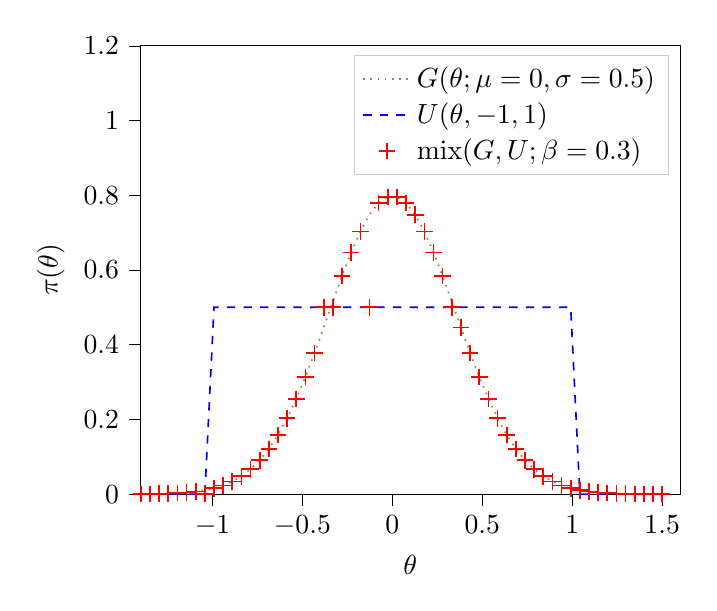
\begin{tikzpicture}

\begin{axis}[
legend cell align={left},
legend style={fill opacity=0.8, draw opacity=1, text opacity=1, draw=white!80!black},
tick align=outside,
tick pos=left,
x grid style={white!69.0196078431373!black},
xlabel={\(\displaystyle \theta\)},
xmin=-1.4, xmax=1.6,
xtick style={color=black},
y grid style={white!69.0196078431373!black},
ylabel={\(\displaystyle \pi(\theta)\)},
ymin=0, ymax=1.2,
ytick style={color=black}
]
\addplot [semithick, yellow!50!black, dotted]
table {%
-1.5 9.8466777332468e-05
-1.44915254237288 0.0001793872435764
-1.39830508474576 0.000320118348094559
-1.34745762711864 0.000559560121531124
-1.29661016949153 0.000958076356441112
-1.24576271186441 0.00160683272401611
-1.19491525423729 0.00263972321036136
-1.14406779661017 0.00424779248787262
-1.09322033898305 0.00669553635076534
-1.04237288135593 0.0103377167883577
-0.991525423728814 0.015634394496712
-0.940677966101695 0.0231608599466659
-0.889830508474576 0.0336082170150122
-0.838983050847458 0.0477698022564135
-0.788135593220339 0.066508720415643
-0.73728813559322 0.0907028470877726
-0.686440677966102 0.121165903387615
-0.635593220338983 0.15854666388776
-0.584745762711864 0.203212757823817
-0.533898305084746 0.255130282294824
-0.483050847457627 0.313754690902936
-0.432203389830508 0.377951108859794
-0.38135593220339 0.445962353038858
-0.330508474576271 0.515439801267037
-0.279661016949152 0.583545711433813
-0.228813559322034 0.647126211028834
-0.177966101694915 0.702943270974129
-0.127118644067796 0.747943415704262
-0.0762711864406778 0.77953278826435
-0.0254237288135593 0.795824323519198
0.0254237288135595 0.795824323519198
0.076271186440678 0.77953278826435
0.127118644067797 0.747943415704262
0.177966101694915 0.702943270974129
0.228813559322034 0.647126211028834
0.279661016949153 0.583545711433812
0.330508474576271 0.515439801267037
0.38135593220339 0.445962353038858
0.432203389830509 0.377951108859794
0.483050847457627 0.313754690902936
0.533898305084746 0.255130282294824
0.584745762711865 0.203212757823817
0.635593220338983 0.15854666388776
0.686440677966102 0.121165903387615
0.737288135593221 0.0907028470877724
0.788135593220339 0.0665087204156429
0.838983050847458 0.0477698022564135
0.889830508474577 0.0336082170150121
0.940677966101695 0.0231608599466659
0.991525423728814 0.015634394496712
1.04237288135593 0.0103377167883577
1.09322033898305 0.00669553635076532
1.14406779661017 0.00424779248787262
1.19491525423729 0.00263972321036135
1.24576271186441 0.0016068327240161
1.29661016949153 0.000958076356441112
1.34745762711864 0.000559560121531121
1.39830508474576 0.000320118348094558
1.44915254237288 0.000179387243576399
1.5 9.8466777332468e-05
};
\addlegendentry{$G(\theta; \mu=0, \sigma=0.5)$}
\addplot [semithick, blue, dashed]
table {%
-1.5 0
-1.44915254237288 0
-1.39830508474576 0
-1.34745762711864 0
-1.29661016949153 0
-1.24576271186441 0
-1.19491525423729 0
-1.14406779661017 0
-1.09322033898305 0
-1.04237288135593 0
-0.991525423728814 0.5
-0.940677966101695 0.5
-0.889830508474576 0.5
-0.838983050847458 0.5
-0.788135593220339 0.5
-0.73728813559322 0.5
-0.686440677966102 0.5
-0.635593220338983 0.5
-0.584745762711864 0.5
-0.533898305084746 0.5
-0.483050847457627 0.5
-0.432203389830508 0.5
-0.38135593220339 0.5
-0.330508474576271 0.5
-0.279661016949152 0.5
-0.228813559322034 0.5
-0.177966101694915 0.5
-0.127118644067796 0.5
-0.0762711864406778 0.5
-0.0254237288135593 0.5
0.0254237288135595 0.5
0.076271186440678 0.5
0.127118644067797 0.5
0.177966101694915 0.5
0.228813559322034 0.5
0.279661016949153 0.5
0.330508474576271 0.5
0.38135593220339 0.5
0.432203389830509 0.5
0.483050847457627 0.5
0.533898305084746 0.5
0.584745762711865 0.5
0.635593220338983 0.5
0.686440677966102 0.5
0.737288135593221 0.5
0.788135593220339 0.5
0.838983050847458 0.5
0.889830508474577 0.5
0.940677966101695 0.5
0.991525423728814 0.5
1.04237288135593 0
1.09322033898305 0
1.14406779661017 0
1.19491525423729 0
1.24576271186441 0
1.29661016949153 0
1.34745762711864 0
1.39830508474576 0
1.44915254237288 0
1.5 0
};
\addlegendentry{$U(\theta, -1, 1)$}
\addplot [semithick, red, mark=+, mark size=3, mark options={solid}, only marks]
table {%
-1.5 9.8466777332468e-05
-1.44915254237288 0.0001793872435764
-1.39830508474576 0
-1.34745762711864 0.000559560121531124
-1.29661016949153 0.000958076356441112
-1.24576271186441 0.00160683272401611
-1.19491525423729 0.00263972321036136
-1.14406779661017 0.00424779248787262
-1.09322033898305 0.00669553635076534
-1.04237288135593 0
-0.991525423728814 0.015634394496712
-0.940677966101695 0.0231608599466659
-0.889830508474576 0.0336082170150122
-0.838983050847458 0.0477698022564135
-0.788135593220339 0.066508720415643
-0.73728813559322 0.0907028470877726
-0.686440677966102 0.121165903387615
-0.635593220338983 0.15854666388776
-0.584745762711864 0.203212757823817
-0.533898305084746 0.255130282294824
-0.483050847457627 0.313754690902936
-0.432203389830508 0.377951108859794
-0.38135593220339 0.5
-0.330508474576271 0.5
-0.279661016949152 0.583545711433813
-0.228813559322034 0.647126211028834
-0.177966101694915 0.702943270974129
-0.127118644067796 0.5
-0.0762711864406778 0.77953278826435
-0.0254237288135593 0.795824323519198
0.0254237288135595 0.795824323519198
0.076271186440678 0.77953278826435
0.127118644067797 0.747943415704262
0.177966101694915 0.702943270974129
0.228813559322034 0.647126211028834
0.279661016949153 0.583545711433812
0.330508474576271 0.5
0.38135593220339 0.445962353038858
0.432203389830509 0.377951108859794
0.483050847457627 0.313754690902936
0.533898305084746 0.255130282294824
0.584745762711865 0.203212757823817
0.635593220338983 0.15854666388776
0.686440677966102 0.121165903387615
0.737288135593221 0.0907028470877724
0.788135593220339 0.0665087204156429
0.838983050847458 0.0477698022564135
0.889830508474577 0.0336082170150121
0.940677966101695 0.0231608599466659
0.991525423728814 0.015634394496712
1.04237288135593 0.0103377167883577
1.09322033898305 0.00669553635076532
1.14406779661017 0.00424779248787262
1.19491525423729 0.00263972321036135
1.24576271186441 0.0016068327240161
1.29661016949153 0.000958076356441112
1.34745762711864 0.000559560121531121
1.39830508474576 0.000320118348094558
1.44915254237288 0.000179387243576399
1.5 9.8466777332468e-05
};
\addlegendentry{mix$(G, U; \beta=0.3)$}
\end{axis}

\end{tikzpicture}

\caption{\label{org87a109a}
An example of a mixture re-partitioning. Notice that the mixture is not normalised to emphasise the coincidence of values with both the uniform distribution and a Gaussian.}
\end{figure}



\section{Method}
\label{sec:org0ea086a}
In this section we shall describe in detail the types of simulations
and bench-marking that was done. As this project is highly
computational, Cosmological issues are discussed only incidentally,
and only with regard to their computational complexity, not the
Physics.

We have chosen to use Cobaya \citep{cobaya}, with CLASS to provide the
theoretical framework for analysing the Planck \citep{planck}
data. Our primary goal is to improve the performance of the
analysis.

We shall first describe how one would measure the performance of
such a run, then show the small-scale simulation results. Finally,
we shall discuss the results obtained by running Cobaya with the
suggested optimisations on the CSD3 cluster (University of Cambridge).


\subsection{Performance and bench-marking}
\label{sec:org304b640}
One cannot use CPU time as a reliable indicator of
performance. There are multiple factors leading to unpredictable
overheads, and these can be practically averaged out on a small
scale model, in case of large distributed systems such as a CPU
cluster, with multiple processes, and with each run taking upwards
of an hour, this metric is beyond the realm usefulness.

Due to the sheer complexity of the Cosmological data and functions
involved in the computation, the usual asymptotic description
common in computer science is insufficient. 

First, note that in Cobaya  the run-time is dominated
by log-likelihood evaluations. A typical run in 3 dimensions
requires \(O(10^{3})\), likelihood calls, and if each of them takes a
second to evaluate, a simple run becomes impractical. 

So a natural choice for a performance metric is using the number of
log-likelihood evaluations. 

Note, however that this does not account for potential extra
complexity introduced by the re-partitioning. For example for PPR,
the effect of adding the extra parameter can be reduced to
\begin{enumerate}
\item one multiplication in the argument of the prior.
\item evaluation of the normalisation factor, which involves standard
numerical functions,
\item addition of the normalisation factor to each log-likelihood call.
\end{enumerate}

The corresponding overhead for mixture modelling is
\begin{enumerate}
\item hashing the vector \(\theta\).
\item generating a pseudo-random number using the hash as seed.
\item performing \(m-1\) conditional checks,
\item addition of \(\ln m\), to the likelihood.
\end{enumerate}

In both cases there's also a minuscule overhead associated with
lengthening the state vector \(\theta\)\footnote{in mixture modelling one could either introduce \(m+1\)
parameters, and perform the hashing once, at the cost of adding an
extra branch index, or add \(m\), parameters but perform the hashing
twice. To choose, mind that the extra branch index parameter, may
adversely impact the convergence as its posterior needs to be computed
just like any other nuisance parameter's.}.  Although these may
become important in low dimensional problems, they are overshadowed
in all practical applications of nested sampling, and thus we shall
ignore them.

\subsection{Correctness}
\label{sec:org88a18ea}
One simple and unreliable way of determining the correctness of a
run is to compare the posteriors of two runs: if the means of two
runs are within one standard deviation of each other, then the
posteriors can be assumed to coincide.

Consider, however, what would happen, if one were to use a Gaussian
prior without posterior re-partitioning on a data set, which was
previously analysed using a uniform prior. One would expect the
posterior to have tighter constraints, smaller variances and for
the evidence to be much higher. Of course, it's normal if said
Gaussian truly represents prior knowledge, but as was mentioned in
previous sections, this is an error for any form of posterior
re-partitioning: it usually means that the re-scaling of the
likelihood is incorrect. Hence we must include (or rather base our
comparison on) the estimated evidences into consideration.

\begin{figure}
% This file was created by tikzplotlib v0.9.1.
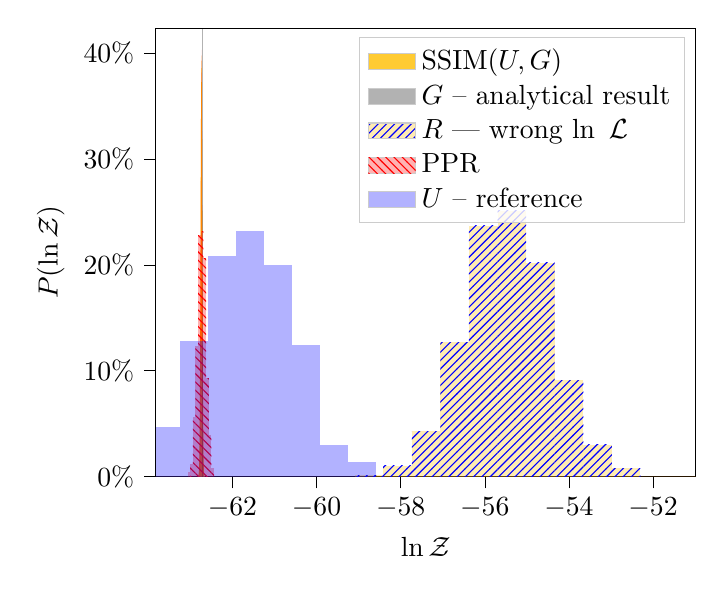
\begin{tikzpicture}

\definecolor{color2}{rgb}{0.0,0.0,1}
\definecolor{color1}{rgb}{1,0.00,0.00}
\definecolor{colorblack}{rgb}{0, 0, 0}
\definecolor{color0}{rgb}{1.0,0.75,0.0}

\begin{axis}[
legend cell align={left},
legend style={fill opacity=0.8, draw opacity=1, text opacity=1, anchor=north east, draw=white!80!black},
tick align=outside,
tick pos=left,
x grid style={white!69.0196078431373!black},
xlabel={\(\ln {\cal Z}\)},
xmin=-63.8198069562379, xmax=-50.9892026507015,
xtick style={color=black},
yticklabel={\pgfmathparse{\tick/10}\pgfmathprintnumber{\pgfmathresult}\%},
y grid style={white!69.0196078431373!black},
ylabel={\(P(\ln {\cal Z})\)},
ymin=0, ymax=423.473092744885,
ytick style={color=black}
]
\path [fill=color0]
(axis cs:-63.8198069562379,0)
--(axis cs:-63.8198069562379,0)
--(axis cs:-63.8069635084846,0)
--(axis cs:-63.7941200607313,0)
--(axis cs:-63.7812766129781,0)
--(axis cs:-63.7684331652248,0)
--(axis cs:-63.7555897174715,0)
--(axis cs:-63.7427462697182,0)
--(axis cs:-63.7299028219649,0)
--(axis cs:-63.7170593742116,0)
--(axis cs:-63.7042159264583,0)
--(axis cs:-63.691372478705,0)
--(axis cs:-63.6785290309517,0)
--(axis cs:-63.6656855831984,0)
--(axis cs:-63.6528421354452,0)
--(axis cs:-63.6399986876919,0)
--(axis cs:-63.6271552399386,0)
--(axis cs:-63.6143117921853,0)
--(axis cs:-63.601468344432,0)
--(axis cs:-63.5886248966787,0)
--(axis cs:-63.5757814489254,0)
--(axis cs:-63.5629380011721,0)
--(axis cs:-63.5500945534188,0)
--(axis cs:-63.5372511056656,0)
--(axis cs:-63.5244076579123,0)
--(axis cs:-63.511564210159,0)
--(axis cs:-63.4987207624057,0)
--(axis cs:-63.4858773146524,0)
--(axis cs:-63.4730338668991,0)
--(axis cs:-63.4601904191458,0)
--(axis cs:-63.4473469713925,0)
--(axis cs:-63.4345035236392,0)
--(axis cs:-63.4216600758859,0)
--(axis cs:-63.4088166281327,0)
--(axis cs:-63.3959731803794,0)
--(axis cs:-63.3831297326261,0)
--(axis cs:-63.3702862848728,0)
--(axis cs:-63.3574428371195,0)
--(axis cs:-63.3445993893662,0)
--(axis cs:-63.3317559416129,0)
--(axis cs:-63.3189124938596,0)
--(axis cs:-63.3060690461063,0)
--(axis cs:-63.293225598353,0)
--(axis cs:-63.2803821505998,0)
--(axis cs:-63.2675387028465,0)
--(axis cs:-63.2546952550932,0)
--(axis cs:-63.2418518073399,0)
--(axis cs:-63.2290083595866,0)
--(axis cs:-63.2161649118333,0)
--(axis cs:-63.20332146408,0)
--(axis cs:-63.1904780163267,0)
--(axis cs:-63.1776345685734,0)
--(axis cs:-63.1647911208201,0)
--(axis cs:-63.1519476730669,0)
--(axis cs:-63.1391042253136,0)
--(axis cs:-63.1262607775603,0)
--(axis cs:-63.113417329807,0)
--(axis cs:-63.1005738820537,0)
--(axis cs:-63.0877304343004,0)
--(axis cs:-63.0748869865471,0)
--(axis cs:-63.0620435387938,0)
--(axis cs:-63.0492000910405,0)
--(axis cs:-63.0363566432872,0)
--(axis cs:-63.023513195534,0)
--(axis cs:-63.0106697477807,0)
--(axis cs:-62.9978263000274,0)
--(axis cs:-62.9849828522741,0)
--(axis cs:-62.9721394045208,0)
--(axis cs:-62.9592959567675,0)
--(axis cs:-62.9464525090142,0)
--(axis cs:-62.9336090612609,0)
--(axis cs:-62.9207656135076,0)
--(axis cs:-62.9079221657544,0)
--(axis cs:-62.8950787180011,0)
--(axis cs:-62.8822352702478,0)
--(axis cs:-62.8693918224945,0)
--(axis cs:-62.8565483747412,0)
--(axis cs:-62.8437049269879,0)
--(axis cs:-62.8308614792346,0)
--(axis cs:-62.8180180314813,0)
--(axis cs:-62.805174583728,0)
--(axis cs:-62.7923311359747,0)
--(axis cs:-62.7794876882215,0)
--(axis cs:-62.7666442404682,0)
--(axis cs:-62.7538007927149,0)
--(axis cs:-62.7409573449616,0)
--(axis cs:-62.7281138972083,0)
--(axis cs:-62.715270449455,0)
--(axis cs:-62.7024270017017,0)
--(axis cs:-62.6895835539484,0)
--(axis cs:-62.6767401061951,0)
--(axis cs:-62.6638966584418,0)
--(axis cs:-62.6510532106886,0)
--(axis cs:-62.6382097629353,0)
--(axis cs:-62.625366315182,0)
--(axis cs:-62.6125228674287,0)
--(axis cs:-62.5996794196754,0)
--(axis cs:-62.5868359719221,0)
--(axis cs:-62.5739925241688,0)
--(axis cs:-62.5611490764155,0)
--(axis cs:-62.5483056286622,0)
--(axis cs:-62.535462180909,0)
--(axis cs:-62.5226187331557,0)
--(axis cs:-62.5097752854024,0)
--(axis cs:-62.4969318376491,0)
--(axis cs:-62.4840883898958,0)
--(axis cs:-62.4712449421425,0)
--(axis cs:-62.4584014943892,0)
--(axis cs:-62.4455580466359,0)
--(axis cs:-62.4327145988826,0)
--(axis cs:-62.4198711511293,0)
--(axis cs:-62.4070277033761,0)
--(axis cs:-62.3941842556228,0)
--(axis cs:-62.3813408078695,0)
--(axis cs:-62.3684973601162,0)
--(axis cs:-62.3556539123629,0)
--(axis cs:-62.3428104646096,0)
--(axis cs:-62.3299670168563,0)
--(axis cs:-62.317123569103,0)
--(axis cs:-62.3042801213497,0)
--(axis cs:-62.2914366735965,0)
--(axis cs:-62.2785932258432,0)
--(axis cs:-62.2657497780899,0)
--(axis cs:-62.2529063303366,0)
--(axis cs:-62.2400628825833,0)
--(axis cs:-62.22721943483,0)
--(axis cs:-62.2143759870767,0)
--(axis cs:-62.2015325393234,0)
--(axis cs:-62.1886890915701,0)
--(axis cs:-62.1758456438168,0)
--(axis cs:-62.1630021960636,0)
--(axis cs:-62.1501587483103,0)
--(axis cs:-62.137315300557,0)
--(axis cs:-62.1244718528037,0)
--(axis cs:-62.1116284050504,0)
--(axis cs:-62.0987849572971,0)
--(axis cs:-62.0859415095438,0)
--(axis cs:-62.0730980617905,0)
--(axis cs:-62.0602546140372,0)
--(axis cs:-62.0474111662839,0)
--(axis cs:-62.0345677185307,0)
--(axis cs:-62.0217242707774,0)
--(axis cs:-62.0088808230241,0)
--(axis cs:-61.9960373752708,0)
--(axis cs:-61.9831939275175,0)
--(axis cs:-61.9703504797642,0)
--(axis cs:-61.9575070320109,0)
--(axis cs:-61.9446635842576,0)
--(axis cs:-61.9318201365043,0)
--(axis cs:-61.918976688751,0)
--(axis cs:-61.9061332409978,0)
--(axis cs:-61.8932897932445,0)
--(axis cs:-61.8804463454912,0)
--(axis cs:-61.8676028977379,0)
--(axis cs:-61.8547594499846,0)
--(axis cs:-61.8419160022313,0)
--(axis cs:-61.829072554478,0)
--(axis cs:-61.8162291067247,0)
--(axis cs:-61.8033856589714,0)
--(axis cs:-61.7905422112181,0)
--(axis cs:-61.7776987634649,0)
--(axis cs:-61.7648553157116,0)
--(axis cs:-61.7520118679583,0)
--(axis cs:-61.739168420205,0)
--(axis cs:-61.7263249724517,0)
--(axis cs:-61.7134815246984,0)
--(axis cs:-61.7006380769451,0)
--(axis cs:-61.6877946291918,0)
--(axis cs:-61.6749511814385,0)
--(axis cs:-61.6621077336853,0)
--(axis cs:-61.649264285932,0)
--(axis cs:-61.6364208381787,0)
--(axis cs:-61.6235773904254,0)
--(axis cs:-61.6107339426721,0)
--(axis cs:-61.5978904949188,0)
--(axis cs:-61.5850470471655,0)
--(axis cs:-61.5722035994122,0)
--(axis cs:-61.5593601516589,0)
--(axis cs:-61.5465167039056,0)
--(axis cs:-61.5336732561524,0)
--(axis cs:-61.5208298083991,0)
--(axis cs:-61.5079863606458,0)
--(axis cs:-61.4951429128925,0)
--(axis cs:-61.4822994651392,0)
--(axis cs:-61.4694560173859,0)
--(axis cs:-61.4566125696326,0)
--(axis cs:-61.4437691218793,0)
--(axis cs:-61.430925674126,0)
--(axis cs:-61.4180822263727,0)
--(axis cs:-61.4052387786195,0)
--(axis cs:-61.3923953308662,0)
--(axis cs:-61.3795518831129,0)
--(axis cs:-61.3667084353596,0)
--(axis cs:-61.3538649876063,0)
--(axis cs:-61.341021539853,0)
--(axis cs:-61.3281780920997,0)
--(axis cs:-61.3153346443464,0)
--(axis cs:-61.3024911965931,0)
--(axis cs:-61.2896477488398,0)
--(axis cs:-61.2768043010866,0)
--(axis cs:-61.2639608533333,0)
--(axis cs:-61.25111740558,0)
--(axis cs:-61.2382739578267,0)
--(axis cs:-61.2254305100734,0)
--(axis cs:-61.2125870623201,0)
--(axis cs:-61.1997436145668,0)
--(axis cs:-61.1869001668135,0)
--(axis cs:-61.1740567190602,0)
--(axis cs:-61.1612132713069,0)
--(axis cs:-61.1483698235537,0)
--(axis cs:-61.1355263758004,0)
--(axis cs:-61.1226829280471,0)
--(axis cs:-61.1098394802938,0)
--(axis cs:-61.0969960325405,0)
--(axis cs:-61.0841525847872,0)
--(axis cs:-61.0713091370339,0)
--(axis cs:-61.0584656892806,0)
--(axis cs:-61.0456222415273,0)
--(axis cs:-61.0327787937741,0)
--(axis cs:-61.0199353460208,0)
--(axis cs:-61.0070918982675,0)
--(axis cs:-60.9942484505142,0)
--(axis cs:-60.9814050027609,0)
--(axis cs:-60.9685615550076,0)
--(axis cs:-60.9557181072543,0)
--(axis cs:-60.942874659501,0)
--(axis cs:-60.9300312117477,0)
--(axis cs:-60.9171877639944,0)
--(axis cs:-60.9043443162412,0)
--(axis cs:-60.8915008684879,0)
--(axis cs:-60.8786574207346,0)
--(axis cs:-60.8658139729813,0)
--(axis cs:-60.852970525228,0)
--(axis cs:-60.8401270774747,0)
--(axis cs:-60.8272836297214,0)
--(axis cs:-60.8144401819681,0)
--(axis cs:-60.8015967342148,0)
--(axis cs:-60.7887532864615,0)
--(axis cs:-60.7759098387083,0)
--(axis cs:-60.763066390955,0)
--(axis cs:-60.7502229432017,0)
--(axis cs:-60.7373794954484,0)
--(axis cs:-60.7245360476951,0)
--(axis cs:-60.7116925999418,0)
--(axis cs:-60.6988491521885,0)
--(axis cs:-60.6860057044352,0)
--(axis cs:-60.6731622566819,0)
--(axis cs:-60.6603188089287,0)
--(axis cs:-60.6474753611754,0)
--(axis cs:-60.6346319134221,0)
--(axis cs:-60.6217884656688,0)
--(axis cs:-60.6089450179155,0)
--(axis cs:-60.5961015701622,0)
--(axis cs:-60.5832581224089,0)
--(axis cs:-60.5704146746556,0)
--(axis cs:-60.5575712269023,0)
--(axis cs:-60.544727779149,0)
--(axis cs:-60.5318843313958,0)
--(axis cs:-60.5190408836425,0)
--(axis cs:-60.5061974358892,0)
--(axis cs:-60.4933539881359,0)
--(axis cs:-60.4805105403826,0)
--(axis cs:-60.4676670926293,0)
--(axis cs:-60.454823644876,0)
--(axis cs:-60.4419801971227,0)
--(axis cs:-60.4291367493694,0)
--(axis cs:-60.4162933016162,0)
--(axis cs:-60.4034498538629,0)
--(axis cs:-60.3906064061096,0)
--(axis cs:-60.3777629583563,0)
--(axis cs:-60.364919510603,0)
--(axis cs:-60.3520760628497,0)
--(axis cs:-60.3392326150964,0)
--(axis cs:-60.3263891673431,0)
--(axis cs:-60.3135457195898,0)
--(axis cs:-60.3007022718365,0)
--(axis cs:-60.2878588240833,0)
--(axis cs:-60.27501537633,0)
--(axis cs:-60.2621719285767,0)
--(axis cs:-60.2493284808234,0)
--(axis cs:-60.2364850330701,0)
--(axis cs:-60.2236415853168,0)
--(axis cs:-60.2107981375635,0)
--(axis cs:-60.1979546898102,0)
--(axis cs:-60.1851112420569,0)
--(axis cs:-60.1722677943036,0)
--(axis cs:-60.1594243465504,0)
--(axis cs:-60.1465808987971,0)
--(axis cs:-60.1337374510438,0)
--(axis cs:-60.1208940032905,0)
--(axis cs:-60.1080505555372,0)
--(axis cs:-60.0952071077839,0)
--(axis cs:-60.0823636600306,0)
--(axis cs:-60.0695202122773,0)
--(axis cs:-60.056676764524,0)
--(axis cs:-60.0438333167707,0)
--(axis cs:-60.0309898690175,0)
--(axis cs:-60.0181464212642,0)
--(axis cs:-60.0053029735109,0)
--(axis cs:-59.9924595257576,0)
--(axis cs:-59.9796160780043,0)
--(axis cs:-59.966772630251,0)
--(axis cs:-59.9539291824977,0)
--(axis cs:-59.9410857347444,0)
--(axis cs:-59.9282422869911,0)
--(axis cs:-59.9153988392378,0)
--(axis cs:-59.9025553914846,0)
--(axis cs:-59.8897119437313,0)
--(axis cs:-59.876868495978,0)
--(axis cs:-59.8640250482247,0)
--(axis cs:-59.8511816004714,0)
--(axis cs:-59.8383381527181,0)
--(axis cs:-59.8254947049648,0)
--(axis cs:-59.8126512572115,0)
--(axis cs:-59.7998078094582,0)
--(axis cs:-59.786964361705,0)
--(axis cs:-59.7741209139517,0)
--(axis cs:-59.7612774661984,0)
--(axis cs:-59.7484340184451,0)
--(axis cs:-59.7355905706918,0)
--(axis cs:-59.7227471229385,0)
--(axis cs:-59.7099036751852,0)
--(axis cs:-59.6970602274319,0)
--(axis cs:-59.6842167796786,0)
--(axis cs:-59.6713733319253,0)
--(axis cs:-59.6585298841721,0)
--(axis cs:-59.6456864364188,0)
--(axis cs:-59.6328429886655,0)
--(axis cs:-59.6199995409122,0)
--(axis cs:-59.6071560931589,0)
--(axis cs:-59.5943126454056,0)
--(axis cs:-59.5814691976523,0)
--(axis cs:-59.568625749899,0)
--(axis cs:-59.5557823021457,0)
--(axis cs:-59.5429388543924,0)
--(axis cs:-59.5300954066392,0)
--(axis cs:-59.5172519588859,0)
--(axis cs:-59.5044085111326,0)
--(axis cs:-59.4915650633793,0)
--(axis cs:-59.478721615626,0)
--(axis cs:-59.4658781678727,0)
--(axis cs:-59.4530347201194,0)
--(axis cs:-59.4401912723661,0)
--(axis cs:-59.4273478246128,0)
--(axis cs:-59.4145043768595,0)
--(axis cs:-59.4016609291063,0)
--(axis cs:-59.388817481353,0)
--(axis cs:-59.3759740335997,0)
--(axis cs:-59.3631305858464,0)
--(axis cs:-59.3502871380931,0)
--(axis cs:-59.3374436903398,0)
--(axis cs:-59.3246002425865,0)
--(axis cs:-59.3117567948332,0)
--(axis cs:-59.2989133470799,0)
--(axis cs:-59.2860698993266,0)
--(axis cs:-59.2732264515734,0)
--(axis cs:-59.2603830038201,0)
--(axis cs:-59.2475395560668,0)
--(axis cs:-59.2346961083135,0)
--(axis cs:-59.2218526605602,0)
--(axis cs:-59.2090092128069,0)
--(axis cs:-59.1961657650536,0)
--(axis cs:-59.1833223173003,0)
--(axis cs:-59.170478869547,0)
--(axis cs:-59.1576354217938,0)
--(axis cs:-59.1447919740405,0)
--(axis cs:-59.1319485262872,0)
--(axis cs:-59.1191050785339,0)
--(axis cs:-59.1062616307806,0)
--(axis cs:-59.0934181830273,0)
--(axis cs:-59.080574735274,0)
--(axis cs:-59.0677312875207,0)
--(axis cs:-59.0548878397674,0)
--(axis cs:-59.0420443920141,0)
--(axis cs:-59.0292009442609,0)
--(axis cs:-59.0163574965076,0)
--(axis cs:-59.0035140487543,0)
--(axis cs:-58.990670601001,0)
--(axis cs:-58.9778271532477,0)
--(axis cs:-58.9649837054944,0)
--(axis cs:-58.9521402577411,0)
--(axis cs:-58.9392968099878,0)
--(axis cs:-58.9264533622345,0)
--(axis cs:-58.9136099144812,0)
--(axis cs:-58.900766466728,0)
--(axis cs:-58.8879230189747,0)
--(axis cs:-58.8750795712214,0)
--(axis cs:-58.8622361234681,0)
--(axis cs:-58.8493926757148,0)
--(axis cs:-58.8365492279615,0)
--(axis cs:-58.8237057802082,0)
--(axis cs:-58.8108623324549,0)
--(axis cs:-58.7980188847016,0)
--(axis cs:-58.7851754369484,0)
--(axis cs:-58.7723319891951,0)
--(axis cs:-58.7594885414418,0)
--(axis cs:-58.7466450936885,0)
--(axis cs:-58.7338016459352,0)
--(axis cs:-58.7209581981819,0)
--(axis cs:-58.7081147504286,0)
--(axis cs:-58.6952713026753,0)
--(axis cs:-58.682427854922,0)
--(axis cs:-58.6695844071687,0)
--(axis cs:-58.6567409594155,0)
--(axis cs:-58.6438975116622,0)
--(axis cs:-58.6310540639089,0)
--(axis cs:-58.6182106161556,0)
--(axis cs:-58.6053671684023,0)
--(axis cs:-58.592523720649,0)
--(axis cs:-58.5796802728957,0)
--(axis cs:-58.5668368251424,0)
--(axis cs:-58.5539933773891,0)
--(axis cs:-58.5411499296358,0)
--(axis cs:-58.5283064818826,0)
--(axis cs:-58.5154630341293,0)
--(axis cs:-58.502619586376,0)
--(axis cs:-58.4897761386227,0)
--(axis cs:-58.4769326908694,0)
--(axis cs:-58.4640892431161,0)
--(axis cs:-58.4512457953628,0)
--(axis cs:-58.4384023476095,0)
--(axis cs:-58.4255588998562,0)
--(axis cs:-58.412715452103,0)
--(axis cs:-58.3998720043497,0)
--(axis cs:-58.3870285565964,0)
--(axis cs:-58.3741851088431,0)
--(axis cs:-58.3613416610898,0)
--(axis cs:-58.3484982133365,0)
--(axis cs:-58.3356547655832,0)
--(axis cs:-58.3228113178299,0)
--(axis cs:-58.3099678700766,0)
--(axis cs:-58.2971244223233,0)
--(axis cs:-58.2842809745701,0)
--(axis cs:-58.2714375268168,0)
--(axis cs:-58.2585940790635,0)
--(axis cs:-58.2457506313102,0)
--(axis cs:-58.2329071835569,0)
--(axis cs:-58.2200637358036,0)
--(axis cs:-58.2072202880503,0)
--(axis cs:-58.194376840297,0)
--(axis cs:-58.1815333925437,0)
--(axis cs:-58.1686899447904,0)
--(axis cs:-58.1558464970372,0)
--(axis cs:-58.1430030492839,0)
--(axis cs:-58.1301596015306,0)
--(axis cs:-58.1173161537773,0)
--(axis cs:-58.104472706024,0)
--(axis cs:-58.0916292582707,0)
--(axis cs:-58.0787858105174,0)
--(axis cs:-58.0659423627641,0)
--(axis cs:-58.0530989150108,0)
--(axis cs:-58.0402554672575,0)
--(axis cs:-58.0274120195043,0)
--(axis cs:-58.014568571751,0)
--(axis cs:-58.0017251239977,0)
--(axis cs:-57.9888816762444,0)
--(axis cs:-57.9760382284911,0)
--(axis cs:-57.9631947807378,0)
--(axis cs:-57.9503513329845,0)
--(axis cs:-57.9375078852312,0)
--(axis cs:-57.9246644374779,0)
--(axis cs:-57.9118209897247,0)
--(axis cs:-57.8989775419714,0)
--(axis cs:-57.8861340942181,0)
--(axis cs:-57.8732906464648,0)
--(axis cs:-57.8604471987115,0)
--(axis cs:-57.8476037509582,0)
--(axis cs:-57.8347603032049,0)
--(axis cs:-57.8219168554516,0)
--(axis cs:-57.8090734076983,0)
--(axis cs:-57.796229959945,0)
--(axis cs:-57.7833865121918,0)
--(axis cs:-57.7705430644385,0)
--(axis cs:-57.7576996166852,0)
--(axis cs:-57.7448561689319,0)
--(axis cs:-57.7320127211786,0)
--(axis cs:-57.7191692734253,0)
--(axis cs:-57.706325825672,0)
--(axis cs:-57.6934823779187,0)
--(axis cs:-57.6806389301654,0)
--(axis cs:-57.6677954824121,0)
--(axis cs:-57.6549520346589,0)
--(axis cs:-57.6421085869056,0)
--(axis cs:-57.6292651391523,0)
--(axis cs:-57.616421691399,0)
--(axis cs:-57.6035782436457,0)
--(axis cs:-57.5907347958924,0)
--(axis cs:-57.5778913481391,0)
--(axis cs:-57.5650479003858,0)
--(axis cs:-57.5522044526325,0)
--(axis cs:-57.5393610048792,0)
--(axis cs:-57.526517557126,0)
--(axis cs:-57.5136741093727,0)
--(axis cs:-57.5008306616194,0)
--(axis cs:-57.4879872138661,0)
--(axis cs:-57.4751437661128,0)
--(axis cs:-57.4623003183595,0)
--(axis cs:-57.4494568706062,0)
--(axis cs:-57.4366134228529,0)
--(axis cs:-57.4237699750996,0)
--(axis cs:-57.4109265273463,0)
--(axis cs:-57.3980830795931,0)
--(axis cs:-57.3852396318398,0)
--(axis cs:-57.3723961840865,0)
--(axis cs:-57.3595527363332,0)
--(axis cs:-57.3467092885799,0)
--(axis cs:-57.3338658408266,0)
--(axis cs:-57.3210223930733,0)
--(axis cs:-57.30817894532,0)
--(axis cs:-57.2953354975667,0)
--(axis cs:-57.2824920498135,0)
--(axis cs:-57.2696486020602,0)
--(axis cs:-57.2568051543069,0)
--(axis cs:-57.2439617065536,0)
--(axis cs:-57.2311182588003,0)
--(axis cs:-57.218274811047,0)
--(axis cs:-57.2054313632937,0)
--(axis cs:-57.1925879155404,0)
--(axis cs:-57.1797444677871,0)
--(axis cs:-57.1669010200338,0)
--(axis cs:-57.1540575722806,0)
--(axis cs:-57.1412141245273,0)
--(axis cs:-57.128370676774,0)
--(axis cs:-57.1155272290207,0)
--(axis cs:-57.1026837812674,0)
--(axis cs:-57.0898403335141,0)
--(axis cs:-57.0769968857608,0)
--(axis cs:-57.0641534380075,0)
--(axis cs:-57.0513099902542,0)
--(axis cs:-57.0384665425009,0)
--(axis cs:-57.0256230947477,0)
--(axis cs:-57.0127796469944,0)
--(axis cs:-56.9999361992411,0)
--(axis cs:-56.9870927514878,0)
--(axis cs:-56.9742493037345,0)
--(axis cs:-56.9614058559812,0)
--(axis cs:-56.9485624082279,0)
--(axis cs:-56.9357189604746,0)
--(axis cs:-56.9228755127213,0)
--(axis cs:-56.910032064968,0)
--(axis cs:-56.8971886172148,0)
--(axis cs:-56.8843451694615,0)
--(axis cs:-56.8715017217082,0)
--(axis cs:-56.8586582739549,0)
--(axis cs:-56.8458148262016,0)
--(axis cs:-56.8329713784483,0)
--(axis cs:-56.820127930695,0)
--(axis cs:-56.8072844829417,0)
--(axis cs:-56.7944410351884,0)
--(axis cs:-56.7815975874352,0)
--(axis cs:-56.7687541396819,0)
--(axis cs:-56.7559106919286,0)
--(axis cs:-56.7430672441753,0)
--(axis cs:-56.730223796422,0)
--(axis cs:-56.7173803486687,0)
--(axis cs:-56.7045369009154,0)
--(axis cs:-56.6916934531621,0)
--(axis cs:-56.6788500054088,0)
--(axis cs:-56.6660065576555,0)
--(axis cs:-56.6531631099023,0)
--(axis cs:-56.640319662149,0)
--(axis cs:-56.6274762143957,0)
--(axis cs:-56.6146327666424,0)
--(axis cs:-56.6017893188891,0)
--(axis cs:-56.5889458711358,0)
--(axis cs:-56.5761024233825,0)
--(axis cs:-56.5632589756292,0)
--(axis cs:-56.5504155278759,0)
--(axis cs:-56.5375720801227,0)
--(axis cs:-56.5247286323694,0)
--(axis cs:-56.5118851846161,0)
--(axis cs:-56.4990417368628,0)
--(axis cs:-56.4861982891095,0)
--(axis cs:-56.4733548413562,0)
--(axis cs:-56.4605113936029,0)
--(axis cs:-56.4476679458496,0)
--(axis cs:-56.4348244980963,0)
--(axis cs:-56.421981050343,0)
--(axis cs:-56.4091376025898,0)
--(axis cs:-56.3962941548365,0)
--(axis cs:-56.3834507070832,0)
--(axis cs:-56.3706072593299,0)
--(axis cs:-56.3577638115766,0)
--(axis cs:-56.3449203638233,0)
--(axis cs:-56.33207691607,0)
--(axis cs:-56.3192334683167,0)
--(axis cs:-56.3063900205634,0)
--(axis cs:-56.2935465728101,0)
--(axis cs:-56.2807031250569,0)
--(axis cs:-56.2678596773036,0)
--(axis cs:-56.2550162295503,0)
--(axis cs:-56.242172781797,0)
--(axis cs:-56.2293293340437,0)
--(axis cs:-56.2164858862904,0)
--(axis cs:-56.2036424385371,0)
--(axis cs:-56.1907989907838,0)
--(axis cs:-56.1779555430305,0)
--(axis cs:-56.1651120952772,0)
--(axis cs:-56.152268647524,0)
--(axis cs:-56.1394251997707,0)
--(axis cs:-56.1265817520174,0)
--(axis cs:-56.1137383042641,0)
--(axis cs:-56.1008948565108,0)
--(axis cs:-56.0880514087575,0)
--(axis cs:-56.0752079610042,0)
--(axis cs:-56.0623645132509,0)
--(axis cs:-56.0495210654976,0)
--(axis cs:-56.0366776177444,0)
--(axis cs:-56.0238341699911,0)
--(axis cs:-56.0109907222378,0)
--(axis cs:-55.9981472744845,0)
--(axis cs:-55.9853038267312,0)
--(axis cs:-55.9724603789779,0)
--(axis cs:-55.9596169312246,0)
--(axis cs:-55.9467734834713,0)
--(axis cs:-55.933930035718,0)
--(axis cs:-55.9210865879647,0)
--(axis cs:-55.9082431402115,0)
--(axis cs:-55.8953996924582,0)
--(axis cs:-55.8825562447049,0)
--(axis cs:-55.8697127969516,0)
--(axis cs:-55.8568693491983,0)
--(axis cs:-55.844025901445,0)
--(axis cs:-55.8311824536917,0)
--(axis cs:-55.8183390059384,0)
--(axis cs:-55.8054955581851,0)
--(axis cs:-55.7926521104318,0)
--(axis cs:-55.7798086626786,0)
--(axis cs:-55.7669652149253,0)
--(axis cs:-55.754121767172,0)
--(axis cs:-55.7412783194187,0)
--(axis cs:-55.7284348716654,0)
--(axis cs:-55.7155914239121,0)
--(axis cs:-55.7027479761588,0)
--(axis cs:-55.6899045284055,0)
--(axis cs:-55.6770610806522,0)
--(axis cs:-55.6642176328989,0)
--(axis cs:-55.6513741851457,0)
--(axis cs:-55.6385307373924,0)
--(axis cs:-55.6256872896391,0)
--(axis cs:-55.6128438418858,0)
--(axis cs:-55.6000003941325,0)
--(axis cs:-55.5871569463792,0)
--(axis cs:-55.5743134986259,0)
--(axis cs:-55.5614700508726,0)
--(axis cs:-55.5486266031193,0)
--(axis cs:-55.535783155366,0)
--(axis cs:-55.5229397076128,0)
--(axis cs:-55.5100962598595,0)
--(axis cs:-55.4972528121062,0)
--(axis cs:-55.4844093643529,0)
--(axis cs:-55.4715659165996,0)
--(axis cs:-55.4587224688463,0)
--(axis cs:-55.445879021093,0)
--(axis cs:-55.4330355733397,0)
--(axis cs:-55.4201921255864,0)
--(axis cs:-55.4073486778332,0)
--(axis cs:-55.3945052300799,0)
--(axis cs:-55.3816617823266,0)
--(axis cs:-55.3688183345733,0)
--(axis cs:-55.35597488682,0)
--(axis cs:-55.3431314390667,0)
--(axis cs:-55.3302879913134,0)
--(axis cs:-55.3174445435601,0)
--(axis cs:-55.3046010958068,0)
--(axis cs:-55.2917576480535,0)
--(axis cs:-55.2789142003003,0)
--(axis cs:-55.266070752547,0)
--(axis cs:-55.2532273047937,0)
--(axis cs:-55.2403838570404,0)
--(axis cs:-55.2275404092871,0)
--(axis cs:-55.2146969615338,0)
--(axis cs:-55.2018535137805,0)
--(axis cs:-55.1890100660272,0)
--(axis cs:-55.1761666182739,0)
--(axis cs:-55.1633231705206,0)
--(axis cs:-55.1504797227674,0)
--(axis cs:-55.1376362750141,0)
--(axis cs:-55.1247928272608,0)
--(axis cs:-55.1119493795075,0)
--(axis cs:-55.0991059317542,0)
--(axis cs:-55.0862624840009,0)
--(axis cs:-55.0734190362476,0)
--(axis cs:-55.0605755884943,0)
--(axis cs:-55.047732140741,0)
--(axis cs:-55.0348886929877,0)
--(axis cs:-55.0220452452345,0)
--(axis cs:-55.0092017974812,0)
--(axis cs:-54.9963583497279,0)
--(axis cs:-54.9835149019746,0)
--(axis cs:-54.9706714542213,0)
--(axis cs:-54.957828006468,0)
--(axis cs:-54.9449845587147,0)
--(axis cs:-54.9321411109614,0)
--(axis cs:-54.9192976632081,0)
--(axis cs:-54.9064542154549,0)
--(axis cs:-54.8936107677016,0)
--(axis cs:-54.8807673199483,0)
--(axis cs:-54.867923872195,0)
--(axis cs:-54.8550804244417,0)
--(axis cs:-54.8422369766884,0)
--(axis cs:-54.8293935289351,0)
--(axis cs:-54.8165500811818,0)
--(axis cs:-54.8037066334285,0)
--(axis cs:-54.7908631856752,0)
--(axis cs:-54.778019737922,0)
--(axis cs:-54.7651762901687,0)
--(axis cs:-54.7523328424154,0)
--(axis cs:-54.7394893946621,0)
--(axis cs:-54.7266459469088,0)
--(axis cs:-54.7138024991555,0)
--(axis cs:-54.7009590514022,0)
--(axis cs:-54.6881156036489,0)
--(axis cs:-54.6752721558956,0)
--(axis cs:-54.6624287081424,0)
--(axis cs:-54.6495852603891,0)
--(axis cs:-54.6367418126358,0)
--(axis cs:-54.6238983648825,0)
--(axis cs:-54.6110549171292,0)
--(axis cs:-54.5982114693759,0)
--(axis cs:-54.5853680216226,0)
--(axis cs:-54.5725245738693,0)
--(axis cs:-54.559681126116,0)
--(axis cs:-54.5468376783627,0)
--(axis cs:-54.5339942306095,0)
--(axis cs:-54.5211507828562,0)
--(axis cs:-54.5083073351029,0)
--(axis cs:-54.4954638873496,0)
--(axis cs:-54.4826204395963,0)
--(axis cs:-54.469776991843,0)
--(axis cs:-54.4569335440897,0)
--(axis cs:-54.4440900963364,0)
--(axis cs:-54.4312466485831,0)
--(axis cs:-54.4184032008298,0)
--(axis cs:-54.4055597530766,0)
--(axis cs:-54.3927163053233,0)
--(axis cs:-54.37987285757,0)
--(axis cs:-54.3670294098167,0)
--(axis cs:-54.3541859620634,0)
--(axis cs:-54.3413425143101,0)
--(axis cs:-54.3284990665568,0)
--(axis cs:-54.3156556188035,0)
--(axis cs:-54.3028121710502,0)
--(axis cs:-54.2899687232969,0)
--(axis cs:-54.2771252755437,0)
--(axis cs:-54.2642818277904,0)
--(axis cs:-54.2514383800371,0)
--(axis cs:-54.2385949322838,0)
--(axis cs:-54.2257514845305,0)
--(axis cs:-54.2129080367772,0)
--(axis cs:-54.2000645890239,0)
--(axis cs:-54.1872211412706,0)
--(axis cs:-54.1743776935173,0)
--(axis cs:-54.161534245764,0)
--(axis cs:-54.1486907980108,0)
--(axis cs:-54.1358473502575,0)
--(axis cs:-54.1230039025042,0)
--(axis cs:-54.1101604547509,0)
--(axis cs:-54.0973170069976,0)
--(axis cs:-54.0844735592443,0)
--(axis cs:-54.071630111491,0)
--(axis cs:-54.0587866637377,0)
--(axis cs:-54.0459432159844,0)
--(axis cs:-54.0330997682312,0)
--(axis cs:-54.0202563204779,0)
--(axis cs:-54.0074128727246,0)
--(axis cs:-53.9945694249713,0)
--(axis cs:-53.981725977218,0)
--(axis cs:-53.9688825294647,0)
--(axis cs:-53.9560390817114,0)
--(axis cs:-53.9431956339581,0)
--(axis cs:-53.9303521862048,0)
--(axis cs:-53.9175087384515,0)
--(axis cs:-53.9046652906983,0)
--(axis cs:-53.891821842945,0)
--(axis cs:-53.8789783951917,0)
--(axis cs:-53.8661349474384,0)
--(axis cs:-53.8532914996851,0)
--(axis cs:-53.8404480519318,0)
--(axis cs:-53.8276046041785,0)
--(axis cs:-53.8147611564252,0)
--(axis cs:-53.8019177086719,0)
--(axis cs:-53.7890742609186,0)
--(axis cs:-53.7762308131654,0)
--(axis cs:-53.7633873654121,0)
--(axis cs:-53.7505439176588,0)
--(axis cs:-53.7377004699055,0)
--(axis cs:-53.7248570221522,0)
--(axis cs:-53.7120135743989,0)
--(axis cs:-53.6991701266456,0)
--(axis cs:-53.6863266788923,0)
--(axis cs:-53.673483231139,0)
--(axis cs:-53.6606397833857,0)
--(axis cs:-53.6477963356325,0)
--(axis cs:-53.6349528878792,0)
--(axis cs:-53.6221094401259,0)
--(axis cs:-53.6092659923726,0)
--(axis cs:-53.5964225446193,0)
--(axis cs:-53.583579096866,0)
--(axis cs:-53.5707356491127,0)
--(axis cs:-53.5578922013594,0)
--(axis cs:-53.5450487536061,0)
--(axis cs:-53.5322053058529,0)
--(axis cs:-53.5193618580996,0)
--(axis cs:-53.5065184103463,0)
--(axis cs:-53.493674962593,0)
--(axis cs:-53.4808315148397,0)
--(axis cs:-53.4679880670864,0)
--(axis cs:-53.4551446193331,0)
--(axis cs:-53.4423011715798,0)
--(axis cs:-53.4294577238265,0)
--(axis cs:-53.4166142760732,0)
--(axis cs:-53.40377082832,0)
--(axis cs:-53.3909273805667,0)
--(axis cs:-53.3780839328134,0)
--(axis cs:-53.3652404850601,0)
--(axis cs:-53.3523970373068,0)
--(axis cs:-53.3395535895535,0)
--(axis cs:-53.3267101418002,0)
--(axis cs:-53.3138666940469,0)
--(axis cs:-53.3010232462936,0)
--(axis cs:-53.2881797985403,0)
--(axis cs:-53.2753363507871,0)
--(axis cs:-53.2624929030338,0)
--(axis cs:-53.2496494552805,0)
--(axis cs:-53.2368060075272,0)
--(axis cs:-53.2239625597739,0)
--(axis cs:-53.2111191120206,0)
--(axis cs:-53.1982756642673,0)
--(axis cs:-53.185432216514,0)
--(axis cs:-53.1725887687607,0)
--(axis cs:-53.1597453210074,0)
--(axis cs:-53.1469018732542,0)
--(axis cs:-53.1340584255009,0)
--(axis cs:-53.1212149777476,0)
--(axis cs:-53.1083715299943,0)
--(axis cs:-53.095528082241,0)
--(axis cs:-53.0826846344877,0)
--(axis cs:-53.0698411867344,0)
--(axis cs:-53.0569977389811,0)
--(axis cs:-53.0441542912278,0)
--(axis cs:-53.0313108434746,0)
--(axis cs:-53.0184673957213,0)
--(axis cs:-53.005623947968,0)
--(axis cs:-52.9927805002147,0)
--(axis cs:-52.9799370524614,0)
--(axis cs:-52.9670936047081,0)
--(axis cs:-52.9542501569548,0)
--(axis cs:-52.9414067092015,0)
--(axis cs:-52.9285632614482,0)
--(axis cs:-52.9157198136949,0)
--(axis cs:-52.9028763659417,0)
--(axis cs:-52.8900329181884,0)
--(axis cs:-52.8771894704351,0)
--(axis cs:-52.8643460226818,0)
--(axis cs:-52.8515025749285,0)
--(axis cs:-52.8386591271752,0)
--(axis cs:-52.8258156794219,0)
--(axis cs:-52.8129722316686,0)
--(axis cs:-52.8001287839153,0)
--(axis cs:-52.787285336162,0)
--(axis cs:-52.7744418884088,0)
--(axis cs:-52.7615984406555,0)
--(axis cs:-52.7487549929022,0)
--(axis cs:-52.7359115451489,0)
--(axis cs:-52.7230680973956,0)
--(axis cs:-52.7102246496423,0)
--(axis cs:-52.697381201889,0)
--(axis cs:-52.6845377541357,0)
--(axis cs:-52.6716943063824,0)
--(axis cs:-52.6588508586292,0)
--(axis cs:-52.6460074108759,0)
--(axis cs:-52.6331639631226,0)
--(axis cs:-52.6203205153693,0)
--(axis cs:-52.607477067616,0)
--(axis cs:-52.5946336198627,0)
--(axis cs:-52.5817901721094,0)
--(axis cs:-52.5689467243561,0)
--(axis cs:-52.5561032766028,0)
--(axis cs:-52.5432598288495,0)
--(axis cs:-52.5304163810963,0)
--(axis cs:-52.517572933343,0)
--(axis cs:-52.5047294855897,0)
--(axis cs:-52.4918860378364,0)
--(axis cs:-52.4790425900831,0)
--(axis cs:-52.4661991423298,0)
--(axis cs:-52.4533556945765,0)
--(axis cs:-52.4405122468232,0)
--(axis cs:-52.4276687990699,0)
--(axis cs:-52.4148253513166,0)
--(axis cs:-52.4019819035634,0)
--(axis cs:-52.3891384558101,0)
--(axis cs:-52.3762950080568,0)
--(axis cs:-52.3634515603035,0)
--(axis cs:-52.3506081125502,0)
--(axis cs:-52.3377646647969,0)
--(axis cs:-52.3249212170436,0)
--(axis cs:-52.3120777692903,0)
--(axis cs:-52.299234321537,0)
--(axis cs:-52.2863908737837,0)
--(axis cs:-52.2735474260305,0)
--(axis cs:-52.2607039782772,0)
--(axis cs:-52.2478605305239,0)
--(axis cs:-52.2350170827706,0)
--(axis cs:-52.2221736350173,0)
--(axis cs:-52.209330187264,0)
--(axis cs:-52.1964867395107,0)
--(axis cs:-52.1836432917574,0)
--(axis cs:-52.1707998440041,0)
--(axis cs:-52.1579563962509,0)
--(axis cs:-52.1451129484976,0)
--(axis cs:-52.1322695007443,0)
--(axis cs:-52.119426052991,0)
--(axis cs:-52.1065826052377,0)
--(axis cs:-52.0937391574844,0)
--(axis cs:-52.0808957097311,0)
--(axis cs:-52.0680522619778,0)
--(axis cs:-52.0552088142245,0)
--(axis cs:-52.0423653664712,0)
--(axis cs:-52.029521918718,0)
--(axis cs:-52.0166784709647,0)
--(axis cs:-52.0038350232114,0)
--(axis cs:-51.9909915754581,0)
--(axis cs:-51.9781481277048,0)
--(axis cs:-51.9653046799515,0)
--(axis cs:-51.9524612321982,0)
--(axis cs:-51.9396177844449,0)
--(axis cs:-51.9267743366916,0)
--(axis cs:-51.9139308889383,0)
--(axis cs:-51.9010874411851,0)
--(axis cs:-51.8882439934318,0)
--(axis cs:-51.8754005456785,0)
--(axis cs:-51.8625570979252,0)
--(axis cs:-51.8497136501719,0)
--(axis cs:-51.8368702024186,0)
--(axis cs:-51.8240267546653,0)
--(axis cs:-51.811183306912,0)
--(axis cs:-51.7983398591587,0)
--(axis cs:-51.7854964114054,0)
--(axis cs:-51.7726529636522,0)
--(axis cs:-51.7598095158989,0)
--(axis cs:-51.7469660681456,0)
--(axis cs:-51.7341226203923,0)
--(axis cs:-51.721279172639,0)
--(axis cs:-51.7084357248857,0)
--(axis cs:-51.6955922771324,0)
--(axis cs:-51.6827488293791,0)
--(axis cs:-51.6699053816258,0)
--(axis cs:-51.6570619338726,0)
--(axis cs:-51.6442184861193,0)
--(axis cs:-51.631375038366,0)
--(axis cs:-51.6185315906127,0)
--(axis cs:-51.6056881428594,0)
--(axis cs:-51.5928446951061,0)
--(axis cs:-51.5800012473528,0)
--(axis cs:-51.5671577995995,0)
--(axis cs:-51.5543143518462,0)
--(axis cs:-51.5414709040929,0)
--(axis cs:-51.5286274563397,0)
--(axis cs:-51.5157840085864,0)
--(axis cs:-51.5029405608331,0)
--(axis cs:-51.4900971130798,0)
--(axis cs:-51.4772536653265,0)
--(axis cs:-51.4644102175732,0)
--(axis cs:-51.4515667698199,0)
--(axis cs:-51.4387233220666,0)
--(axis cs:-51.4258798743133,0)
--(axis cs:-51.41303642656,0)
--(axis cs:-51.4001929788068,0)
--(axis cs:-51.3873495310535,0)
--(axis cs:-51.3745060833002,0)
--(axis cs:-51.3616626355469,0)
--(axis cs:-51.3488191877936,0)
--(axis cs:-51.3359757400403,0)
--(axis cs:-51.323132292287,0)
--(axis cs:-51.3102888445337,0)
--(axis cs:-51.2974453967804,0)
--(axis cs:-51.2846019490271,0)
--(axis cs:-51.2717585012739,0)
--(axis cs:-51.2589150535206,0)
--(axis cs:-51.2460716057673,0)
--(axis cs:-51.233228158014,0)
--(axis cs:-51.2203847102607,0)
--(axis cs:-51.2075412625074,0)
--(axis cs:-51.1946978147541,0)
--(axis cs:-51.1818543670008,0)
--(axis cs:-51.1690109192475,0)
--(axis cs:-51.1561674714942,0)
--(axis cs:-51.143324023741,0)
--(axis cs:-51.1304805759877,0)
--(axis cs:-51.1176371282344,0)
--(axis cs:-51.1047936804811,0)
--(axis cs:-51.0919502327278,0)
--(axis cs:-51.0791067849745,0)
--(axis cs:-51.0662633372212,0)
--(axis cs:-51.0534198894679,0)
--(axis cs:-51.0405764417146,0)
--(axis cs:-51.0277329939614,0)
--(axis cs:-51.0148895462081,0)
--(axis cs:-51.0020460984548,0)
--(axis cs:-50.9892026507015,0)
--(axis cs:-50.9892026507015,0)
--(axis cs:-50.9892026507015,0)
--(axis cs:-51.0020460984548,0)
--(axis cs:-51.0148895462081,0)
--(axis cs:-51.0277329939614,0)
--(axis cs:-51.0405764417146,0)
--(axis cs:-51.0534198894679,0)
--(axis cs:-51.0662633372212,0)
--(axis cs:-51.0791067849745,0)
--(axis cs:-51.0919502327278,0)
--(axis cs:-51.1047936804811,0)
--(axis cs:-51.1176371282344,0)
--(axis cs:-51.1304805759877,0)
--(axis cs:-51.143324023741,0)
--(axis cs:-51.1561674714942,0)
--(axis cs:-51.1690109192475,0)
--(axis cs:-51.1818543670008,0)
--(axis cs:-51.1946978147541,0)
--(axis cs:-51.2075412625074,0)
--(axis cs:-51.2203847102607,0)
--(axis cs:-51.233228158014,0)
--(axis cs:-51.2460716057673,0)
--(axis cs:-51.2589150535206,0)
--(axis cs:-51.2717585012739,0)
--(axis cs:-51.2846019490271,0)
--(axis cs:-51.2974453967804,0)
--(axis cs:-51.3102888445337,0)
--(axis cs:-51.323132292287,0)
--(axis cs:-51.3359757400403,0)
--(axis cs:-51.3488191877936,0)
--(axis cs:-51.3616626355469,0)
--(axis cs:-51.3745060833002,0)
--(axis cs:-51.3873495310535,0)
--(axis cs:-51.4001929788068,0)
--(axis cs:-51.41303642656,0)
--(axis cs:-51.4258798743133,0)
--(axis cs:-51.4387233220666,0)
--(axis cs:-51.4515667698199,0)
--(axis cs:-51.4644102175732,0)
--(axis cs:-51.4772536653265,0)
--(axis cs:-51.4900971130798,0)
--(axis cs:-51.5029405608331,0)
--(axis cs:-51.5157840085864,0)
--(axis cs:-51.5286274563397,0)
--(axis cs:-51.5414709040929,0)
--(axis cs:-51.5543143518462,0)
--(axis cs:-51.5671577995995,0)
--(axis cs:-51.5800012473528,0)
--(axis cs:-51.5928446951061,0)
--(axis cs:-51.6056881428594,0)
--(axis cs:-51.6185315906127,0)
--(axis cs:-51.631375038366,0)
--(axis cs:-51.6442184861193,0)
--(axis cs:-51.6570619338726,0)
--(axis cs:-51.6699053816258,0)
--(axis cs:-51.6827488293791,0)
--(axis cs:-51.6955922771324,0)
--(axis cs:-51.7084357248857,0)
--(axis cs:-51.721279172639,0)
--(axis cs:-51.7341226203923,0)
--(axis cs:-51.7469660681456,0)
--(axis cs:-51.7598095158989,0)
--(axis cs:-51.7726529636522,0)
--(axis cs:-51.7854964114054,0)
--(axis cs:-51.7983398591587,0)
--(axis cs:-51.811183306912,0)
--(axis cs:-51.8240267546653,0)
--(axis cs:-51.8368702024186,0)
--(axis cs:-51.8497136501719,0)
--(axis cs:-51.8625570979252,0)
--(axis cs:-51.8754005456785,0)
--(axis cs:-51.8882439934318,0)
--(axis cs:-51.9010874411851,0)
--(axis cs:-51.9139308889383,0)
--(axis cs:-51.9267743366916,0)
--(axis cs:-51.9396177844449,0)
--(axis cs:-51.9524612321982,0)
--(axis cs:-51.9653046799515,0)
--(axis cs:-51.9781481277048,0)
--(axis cs:-51.9909915754581,0)
--(axis cs:-52.0038350232114,0)
--(axis cs:-52.0166784709647,0)
--(axis cs:-52.029521918718,0)
--(axis cs:-52.0423653664712,0)
--(axis cs:-52.0552088142245,0)
--(axis cs:-52.0680522619778,0)
--(axis cs:-52.0808957097311,0)
--(axis cs:-52.0937391574844,0)
--(axis cs:-52.1065826052377,0)
--(axis cs:-52.119426052991,0)
--(axis cs:-52.1322695007443,0)
--(axis cs:-52.1451129484976,0)
--(axis cs:-52.1579563962509,0)
--(axis cs:-52.1707998440041,0)
--(axis cs:-52.1836432917574,0)
--(axis cs:-52.1964867395107,0)
--(axis cs:-52.209330187264,0)
--(axis cs:-52.2221736350173,0)
--(axis cs:-52.2350170827706,0)
--(axis cs:-52.2478605305239,0)
--(axis cs:-52.2607039782772,0)
--(axis cs:-52.2735474260305,0)
--(axis cs:-52.2863908737837,0)
--(axis cs:-52.299234321537,0)
--(axis cs:-52.3120777692903,0)
--(axis cs:-52.3249212170436,0)
--(axis cs:-52.3377646647969,0)
--(axis cs:-52.3506081125502,0)
--(axis cs:-52.3634515603035,0)
--(axis cs:-52.3762950080568,0)
--(axis cs:-52.3891384558101,0)
--(axis cs:-52.4019819035634,0)
--(axis cs:-52.4148253513166,0)
--(axis cs:-52.4276687990699,0)
--(axis cs:-52.4405122468232,0)
--(axis cs:-52.4533556945765,0)
--(axis cs:-52.4661991423298,0)
--(axis cs:-52.4790425900831,0)
--(axis cs:-52.4918860378364,0)
--(axis cs:-52.5047294855897,0)
--(axis cs:-52.517572933343,0)
--(axis cs:-52.5304163810963,0)
--(axis cs:-52.5432598288495,0)
--(axis cs:-52.5561032766028,0)
--(axis cs:-52.5689467243561,0)
--(axis cs:-52.5817901721094,0)
--(axis cs:-52.5946336198627,0)
--(axis cs:-52.607477067616,0)
--(axis cs:-52.6203205153693,0)
--(axis cs:-52.6331639631226,0)
--(axis cs:-52.6460074108759,0)
--(axis cs:-52.6588508586292,0)
--(axis cs:-52.6716943063824,0)
--(axis cs:-52.6845377541357,0)
--(axis cs:-52.697381201889,0)
--(axis cs:-52.7102246496423,0)
--(axis cs:-52.7230680973956,0)
--(axis cs:-52.7359115451489,0)
--(axis cs:-52.7487549929022,0)
--(axis cs:-52.7615984406555,0)
--(axis cs:-52.7744418884088,0)
--(axis cs:-52.787285336162,0)
--(axis cs:-52.8001287839153,0)
--(axis cs:-52.8129722316686,0)
--(axis cs:-52.8258156794219,0)
--(axis cs:-52.8386591271752,0)
--(axis cs:-52.8515025749285,0)
--(axis cs:-52.8643460226818,0)
--(axis cs:-52.8771894704351,0)
--(axis cs:-52.8900329181884,0)
--(axis cs:-52.9028763659417,0)
--(axis cs:-52.9157198136949,0)
--(axis cs:-52.9285632614482,0)
--(axis cs:-52.9414067092015,0)
--(axis cs:-52.9542501569548,0)
--(axis cs:-52.9670936047081,0)
--(axis cs:-52.9799370524614,0)
--(axis cs:-52.9927805002147,0)
--(axis cs:-53.005623947968,0)
--(axis cs:-53.0184673957213,0)
--(axis cs:-53.0313108434746,0)
--(axis cs:-53.0441542912278,0)
--(axis cs:-53.0569977389811,0)
--(axis cs:-53.0698411867344,0)
--(axis cs:-53.0826846344877,0)
--(axis cs:-53.095528082241,0)
--(axis cs:-53.1083715299943,0)
--(axis cs:-53.1212149777476,0)
--(axis cs:-53.1340584255009,0)
--(axis cs:-53.1469018732542,0)
--(axis cs:-53.1597453210074,0)
--(axis cs:-53.1725887687607,0)
--(axis cs:-53.185432216514,0)
--(axis cs:-53.1982756642673,0)
--(axis cs:-53.2111191120206,0)
--(axis cs:-53.2239625597739,0)
--(axis cs:-53.2368060075272,0)
--(axis cs:-53.2496494552805,0)
--(axis cs:-53.2624929030338,0)
--(axis cs:-53.2753363507871,0)
--(axis cs:-53.2881797985403,0)
--(axis cs:-53.3010232462936,0)
--(axis cs:-53.3138666940469,0)
--(axis cs:-53.3267101418002,0)
--(axis cs:-53.3395535895535,0)
--(axis cs:-53.3523970373068,0)
--(axis cs:-53.3652404850601,0)
--(axis cs:-53.3780839328134,0)
--(axis cs:-53.3909273805667,0)
--(axis cs:-53.40377082832,0)
--(axis cs:-53.4166142760732,0)
--(axis cs:-53.4294577238265,0)
--(axis cs:-53.4423011715798,0)
--(axis cs:-53.4551446193331,0)
--(axis cs:-53.4679880670864,0)
--(axis cs:-53.4808315148397,0)
--(axis cs:-53.493674962593,0)
--(axis cs:-53.5065184103463,0)
--(axis cs:-53.5193618580996,0)
--(axis cs:-53.5322053058529,0)
--(axis cs:-53.5450487536061,0)
--(axis cs:-53.5578922013594,0)
--(axis cs:-53.5707356491127,0)
--(axis cs:-53.583579096866,0)
--(axis cs:-53.5964225446193,0)
--(axis cs:-53.6092659923726,0)
--(axis cs:-53.6221094401259,0)
--(axis cs:-53.6349528878792,0)
--(axis cs:-53.6477963356325,0)
--(axis cs:-53.6606397833857,0)
--(axis cs:-53.673483231139,0)
--(axis cs:-53.6863266788923,0)
--(axis cs:-53.6991701266456,0)
--(axis cs:-53.7120135743989,0)
--(axis cs:-53.7248570221522,0)
--(axis cs:-53.7377004699055,0)
--(axis cs:-53.7505439176588,0)
--(axis cs:-53.7633873654121,0)
--(axis cs:-53.7762308131654,0)
--(axis cs:-53.7890742609186,0)
--(axis cs:-53.8019177086719,0)
--(axis cs:-53.8147611564252,0)
--(axis cs:-53.8276046041785,0)
--(axis cs:-53.8404480519318,0)
--(axis cs:-53.8532914996851,0)
--(axis cs:-53.8661349474384,0)
--(axis cs:-53.8789783951917,0)
--(axis cs:-53.891821842945,0)
--(axis cs:-53.9046652906983,0)
--(axis cs:-53.9175087384515,0)
--(axis cs:-53.9303521862048,0)
--(axis cs:-53.9431956339581,0)
--(axis cs:-53.9560390817114,0)
--(axis cs:-53.9688825294647,0)
--(axis cs:-53.981725977218,0)
--(axis cs:-53.9945694249713,0)
--(axis cs:-54.0074128727246,0)
--(axis cs:-54.0202563204779,0)
--(axis cs:-54.0330997682312,0)
--(axis cs:-54.0459432159844,0)
--(axis cs:-54.0587866637377,0)
--(axis cs:-54.071630111491,0)
--(axis cs:-54.0844735592443,0)
--(axis cs:-54.0973170069976,0)
--(axis cs:-54.1101604547509,0)
--(axis cs:-54.1230039025042,0)
--(axis cs:-54.1358473502575,0)
--(axis cs:-54.1486907980108,0)
--(axis cs:-54.161534245764,0)
--(axis cs:-54.1743776935173,0)
--(axis cs:-54.1872211412706,0)
--(axis cs:-54.2000645890239,0)
--(axis cs:-54.2129080367772,0)
--(axis cs:-54.2257514845305,0)
--(axis cs:-54.2385949322838,0)
--(axis cs:-54.2514383800371,0)
--(axis cs:-54.2642818277904,0)
--(axis cs:-54.2771252755437,0)
--(axis cs:-54.2899687232969,0)
--(axis cs:-54.3028121710502,0)
--(axis cs:-54.3156556188035,0)
--(axis cs:-54.3284990665568,0)
--(axis cs:-54.3413425143101,0)
--(axis cs:-54.3541859620634,0)
--(axis cs:-54.3670294098167,0)
--(axis cs:-54.37987285757,0)
--(axis cs:-54.3927163053233,0)
--(axis cs:-54.4055597530766,0)
--(axis cs:-54.4184032008298,0)
--(axis cs:-54.4312466485831,0)
--(axis cs:-54.4440900963364,0)
--(axis cs:-54.4569335440897,0)
--(axis cs:-54.469776991843,0)
--(axis cs:-54.4826204395963,0)
--(axis cs:-54.4954638873496,0)
--(axis cs:-54.5083073351029,0)
--(axis cs:-54.5211507828562,0)
--(axis cs:-54.5339942306095,0)
--(axis cs:-54.5468376783627,0)
--(axis cs:-54.559681126116,0)
--(axis cs:-54.5725245738693,0)
--(axis cs:-54.5853680216226,0)
--(axis cs:-54.5982114693759,0)
--(axis cs:-54.6110549171292,0)
--(axis cs:-54.6238983648825,0)
--(axis cs:-54.6367418126358,0)
--(axis cs:-54.6495852603891,0)
--(axis cs:-54.6624287081424,0)
--(axis cs:-54.6752721558956,0)
--(axis cs:-54.6881156036489,0)
--(axis cs:-54.7009590514022,0)
--(axis cs:-54.7138024991555,0)
--(axis cs:-54.7266459469088,0)
--(axis cs:-54.7394893946621,0)
--(axis cs:-54.7523328424154,0)
--(axis cs:-54.7651762901687,0)
--(axis cs:-54.778019737922,0)
--(axis cs:-54.7908631856752,0)
--(axis cs:-54.8037066334285,0)
--(axis cs:-54.8165500811818,0)
--(axis cs:-54.8293935289351,0)
--(axis cs:-54.8422369766884,0)
--(axis cs:-54.8550804244417,0)
--(axis cs:-54.867923872195,0)
--(axis cs:-54.8807673199483,0)
--(axis cs:-54.8936107677016,0)
--(axis cs:-54.9064542154549,0)
--(axis cs:-54.9192976632081,0)
--(axis cs:-54.9321411109614,0)
--(axis cs:-54.9449845587147,0)
--(axis cs:-54.957828006468,0)
--(axis cs:-54.9706714542213,0)
--(axis cs:-54.9835149019746,0)
--(axis cs:-54.9963583497279,0)
--(axis cs:-55.0092017974812,0)
--(axis cs:-55.0220452452345,0)
--(axis cs:-55.0348886929877,0)
--(axis cs:-55.047732140741,0)
--(axis cs:-55.0605755884943,0)
--(axis cs:-55.0734190362476,0)
--(axis cs:-55.0862624840009,0)
--(axis cs:-55.0991059317542,0)
--(axis cs:-55.1119493795075,0)
--(axis cs:-55.1247928272608,0)
--(axis cs:-55.1376362750141,0)
--(axis cs:-55.1504797227674,0)
--(axis cs:-55.1633231705206,0)
--(axis cs:-55.1761666182739,0)
--(axis cs:-55.1890100660272,0)
--(axis cs:-55.2018535137805,0)
--(axis cs:-55.2146969615338,0)
--(axis cs:-55.2275404092871,0)
--(axis cs:-55.2403838570404,0)
--(axis cs:-55.2532273047937,0)
--(axis cs:-55.266070752547,0)
--(axis cs:-55.2789142003003,0)
--(axis cs:-55.2917576480535,0)
--(axis cs:-55.3046010958068,0)
--(axis cs:-55.3174445435601,0)
--(axis cs:-55.3302879913134,0)
--(axis cs:-55.3431314390667,0)
--(axis cs:-55.35597488682,0)
--(axis cs:-55.3688183345733,0)
--(axis cs:-55.3816617823266,0)
--(axis cs:-55.3945052300799,0)
--(axis cs:-55.4073486778332,0)
--(axis cs:-55.4201921255864,0)
--(axis cs:-55.4330355733397,0)
--(axis cs:-55.445879021093,0)
--(axis cs:-55.4587224688463,0)
--(axis cs:-55.4715659165996,0)
--(axis cs:-55.4844093643529,0)
--(axis cs:-55.4972528121062,0)
--(axis cs:-55.5100962598595,0)
--(axis cs:-55.5229397076128,0)
--(axis cs:-55.535783155366,0)
--(axis cs:-55.5486266031193,0)
--(axis cs:-55.5614700508726,0)
--(axis cs:-55.5743134986259,0)
--(axis cs:-55.5871569463792,0)
--(axis cs:-55.6000003941325,0)
--(axis cs:-55.6128438418858,0)
--(axis cs:-55.6256872896391,0)
--(axis cs:-55.6385307373924,0)
--(axis cs:-55.6513741851457,0)
--(axis cs:-55.6642176328989,0)
--(axis cs:-55.6770610806522,0)
--(axis cs:-55.6899045284055,0)
--(axis cs:-55.7027479761588,0)
--(axis cs:-55.7155914239121,0)
--(axis cs:-55.7284348716654,0)
--(axis cs:-55.7412783194187,0)
--(axis cs:-55.754121767172,0)
--(axis cs:-55.7669652149253,0)
--(axis cs:-55.7798086626786,0)
--(axis cs:-55.7926521104318,0)
--(axis cs:-55.8054955581851,0)
--(axis cs:-55.8183390059384,0)
--(axis cs:-55.8311824536917,0)
--(axis cs:-55.844025901445,0)
--(axis cs:-55.8568693491983,0)
--(axis cs:-55.8697127969516,0)
--(axis cs:-55.8825562447049,0)
--(axis cs:-55.8953996924582,0)
--(axis cs:-55.9082431402115,0)
--(axis cs:-55.9210865879647,0)
--(axis cs:-55.933930035718,0)
--(axis cs:-55.9467734834713,0)
--(axis cs:-55.9596169312246,0)
--(axis cs:-55.9724603789779,0)
--(axis cs:-55.9853038267312,0)
--(axis cs:-55.9981472744845,0)
--(axis cs:-56.0109907222378,0)
--(axis cs:-56.0238341699911,0)
--(axis cs:-56.0366776177444,0)
--(axis cs:-56.0495210654976,0)
--(axis cs:-56.0623645132509,0)
--(axis cs:-56.0752079610042,0)
--(axis cs:-56.0880514087575,0)
--(axis cs:-56.1008948565108,0)
--(axis cs:-56.1137383042641,0)
--(axis cs:-56.1265817520174,0)
--(axis cs:-56.1394251997707,0)
--(axis cs:-56.152268647524,0)
--(axis cs:-56.1651120952772,0)
--(axis cs:-56.1779555430305,0)
--(axis cs:-56.1907989907838,0)
--(axis cs:-56.2036424385371,0)
--(axis cs:-56.2164858862904,0)
--(axis cs:-56.2293293340437,0)
--(axis cs:-56.242172781797,0)
--(axis cs:-56.2550162295503,0)
--(axis cs:-56.2678596773036,0)
--(axis cs:-56.2807031250569,0)
--(axis cs:-56.2935465728101,0)
--(axis cs:-56.3063900205634,0)
--(axis cs:-56.3192334683167,0)
--(axis cs:-56.33207691607,0)
--(axis cs:-56.3449203638233,0)
--(axis cs:-56.3577638115766,0)
--(axis cs:-56.3706072593299,0)
--(axis cs:-56.3834507070832,0)
--(axis cs:-56.3962941548365,0)
--(axis cs:-56.4091376025898,0)
--(axis cs:-56.421981050343,0)
--(axis cs:-56.4348244980963,0)
--(axis cs:-56.4476679458496,0)
--(axis cs:-56.4605113936029,0)
--(axis cs:-56.4733548413562,0)
--(axis cs:-56.4861982891095,0)
--(axis cs:-56.4990417368628,0)
--(axis cs:-56.5118851846161,0)
--(axis cs:-56.5247286323694,0)
--(axis cs:-56.5375720801227,0)
--(axis cs:-56.5504155278759,0)
--(axis cs:-56.5632589756292,0)
--(axis cs:-56.5761024233825,0)
--(axis cs:-56.5889458711358,0)
--(axis cs:-56.6017893188891,0)
--(axis cs:-56.6146327666424,0)
--(axis cs:-56.6274762143957,0)
--(axis cs:-56.640319662149,0)
--(axis cs:-56.6531631099023,0)
--(axis cs:-56.6660065576555,0)
--(axis cs:-56.6788500054088,0)
--(axis cs:-56.6916934531621,0)
--(axis cs:-56.7045369009154,0)
--(axis cs:-56.7173803486687,0)
--(axis cs:-56.730223796422,0)
--(axis cs:-56.7430672441753,0)
--(axis cs:-56.7559106919286,0)
--(axis cs:-56.7687541396819,0)
--(axis cs:-56.7815975874352,0)
--(axis cs:-56.7944410351884,0)
--(axis cs:-56.8072844829417,0)
--(axis cs:-56.820127930695,0)
--(axis cs:-56.8329713784483,0)
--(axis cs:-56.8458148262016,0)
--(axis cs:-56.8586582739549,0)
--(axis cs:-56.8715017217082,0)
--(axis cs:-56.8843451694615,0)
--(axis cs:-56.8971886172148,0)
--(axis cs:-56.910032064968,0)
--(axis cs:-56.9228755127213,0)
--(axis cs:-56.9357189604746,0)
--(axis cs:-56.9485624082279,0)
--(axis cs:-56.9614058559812,0)
--(axis cs:-56.9742493037345,0)
--(axis cs:-56.9870927514878,0)
--(axis cs:-56.9999361992411,0)
--(axis cs:-57.0127796469944,0)
--(axis cs:-57.0256230947477,0)
--(axis cs:-57.0384665425009,0)
--(axis cs:-57.0513099902542,0)
--(axis cs:-57.0641534380075,0)
--(axis cs:-57.0769968857608,0)
--(axis cs:-57.0898403335141,0)
--(axis cs:-57.1026837812674,0)
--(axis cs:-57.1155272290207,0)
--(axis cs:-57.128370676774,0)
--(axis cs:-57.1412141245273,0)
--(axis cs:-57.1540575722806,0)
--(axis cs:-57.1669010200338,0)
--(axis cs:-57.1797444677871,0)
--(axis cs:-57.1925879155404,0)
--(axis cs:-57.2054313632937,0)
--(axis cs:-57.218274811047,0)
--(axis cs:-57.2311182588003,0)
--(axis cs:-57.2439617065536,0)
--(axis cs:-57.2568051543069,0)
--(axis cs:-57.2696486020602,0)
--(axis cs:-57.2824920498135,0)
--(axis cs:-57.2953354975667,0)
--(axis cs:-57.30817894532,0)
--(axis cs:-57.3210223930733,0)
--(axis cs:-57.3338658408266,0)
--(axis cs:-57.3467092885799,0)
--(axis cs:-57.3595527363332,0)
--(axis cs:-57.3723961840865,0)
--(axis cs:-57.3852396318398,0)
--(axis cs:-57.3980830795931,0)
--(axis cs:-57.4109265273463,0)
--(axis cs:-57.4237699750996,0)
--(axis cs:-57.4366134228529,0)
--(axis cs:-57.4494568706062,0)
--(axis cs:-57.4623003183595,0)
--(axis cs:-57.4751437661128,0)
--(axis cs:-57.4879872138661,0)
--(axis cs:-57.5008306616194,0)
--(axis cs:-57.5136741093727,0)
--(axis cs:-57.526517557126,0)
--(axis cs:-57.5393610048792,0)
--(axis cs:-57.5522044526325,0)
--(axis cs:-57.5650479003858,0)
--(axis cs:-57.5778913481391,0)
--(axis cs:-57.5907347958924,0)
--(axis cs:-57.6035782436457,0)
--(axis cs:-57.616421691399,0)
--(axis cs:-57.6292651391523,0)
--(axis cs:-57.6421085869056,0)
--(axis cs:-57.6549520346589,0)
--(axis cs:-57.6677954824121,0)
--(axis cs:-57.6806389301654,0)
--(axis cs:-57.6934823779187,0)
--(axis cs:-57.706325825672,0)
--(axis cs:-57.7191692734253,0)
--(axis cs:-57.7320127211786,0)
--(axis cs:-57.7448561689319,0)
--(axis cs:-57.7576996166852,0)
--(axis cs:-57.7705430644385,0)
--(axis cs:-57.7833865121918,0)
--(axis cs:-57.796229959945,0)
--(axis cs:-57.8090734076983,0)
--(axis cs:-57.8219168554516,0)
--(axis cs:-57.8347603032049,0)
--(axis cs:-57.8476037509582,0)
--(axis cs:-57.8604471987115,0)
--(axis cs:-57.8732906464648,0)
--(axis cs:-57.8861340942181,0)
--(axis cs:-57.8989775419714,0)
--(axis cs:-57.9118209897247,0)
--(axis cs:-57.9246644374779,0)
--(axis cs:-57.9375078852312,0)
--(axis cs:-57.9503513329845,0)
--(axis cs:-57.9631947807378,0)
--(axis cs:-57.9760382284911,0)
--(axis cs:-57.9888816762444,0)
--(axis cs:-58.0017251239977,0)
--(axis cs:-58.014568571751,0)
--(axis cs:-58.0274120195043,0)
--(axis cs:-58.0402554672575,0)
--(axis cs:-58.0530989150108,0)
--(axis cs:-58.0659423627641,0)
--(axis cs:-58.0787858105174,0)
--(axis cs:-58.0916292582707,0)
--(axis cs:-58.104472706024,0)
--(axis cs:-58.1173161537773,0)
--(axis cs:-58.1301596015306,0)
--(axis cs:-58.1430030492839,0)
--(axis cs:-58.1558464970372,0)
--(axis cs:-58.1686899447904,0)
--(axis cs:-58.1815333925437,0)
--(axis cs:-58.194376840297,0)
--(axis cs:-58.2072202880503,0)
--(axis cs:-58.2200637358036,0)
--(axis cs:-58.2329071835569,0)
--(axis cs:-58.2457506313102,0)
--(axis cs:-58.2585940790635,0)
--(axis cs:-58.2714375268168,0)
--(axis cs:-58.2842809745701,0)
--(axis cs:-58.2971244223233,0)
--(axis cs:-58.3099678700766,0)
--(axis cs:-58.3228113178299,0)
--(axis cs:-58.3356547655832,0)
--(axis cs:-58.3484982133365,0)
--(axis cs:-58.3613416610898,0)
--(axis cs:-58.3741851088431,0)
--(axis cs:-58.3870285565964,0)
--(axis cs:-58.3998720043497,0)
--(axis cs:-58.412715452103,0)
--(axis cs:-58.4255588998562,0)
--(axis cs:-58.4384023476095,0)
--(axis cs:-58.4512457953628,0)
--(axis cs:-58.4640892431161,0)
--(axis cs:-58.4769326908694,0)
--(axis cs:-58.4897761386227,0)
--(axis cs:-58.502619586376,0)
--(axis cs:-58.5154630341293,0)
--(axis cs:-58.5283064818826,0)
--(axis cs:-58.5411499296358,0)
--(axis cs:-58.5539933773891,0)
--(axis cs:-58.5668368251424,0)
--(axis cs:-58.5796802728957,0)
--(axis cs:-58.592523720649,0)
--(axis cs:-58.6053671684023,0)
--(axis cs:-58.6182106161556,0)
--(axis cs:-58.6310540639089,0)
--(axis cs:-58.6438975116622,0)
--(axis cs:-58.6567409594155,0)
--(axis cs:-58.6695844071687,0)
--(axis cs:-58.682427854922,0)
--(axis cs:-58.6952713026753,0)
--(axis cs:-58.7081147504286,0)
--(axis cs:-58.7209581981819,0)
--(axis cs:-58.7338016459352,0)
--(axis cs:-58.7466450936885,0)
--(axis cs:-58.7594885414418,0)
--(axis cs:-58.7723319891951,0)
--(axis cs:-58.7851754369484,0)
--(axis cs:-58.7980188847016,0)
--(axis cs:-58.8108623324549,0)
--(axis cs:-58.8237057802082,0)
--(axis cs:-58.8365492279615,0)
--(axis cs:-58.8493926757148,0)
--(axis cs:-58.8622361234681,0)
--(axis cs:-58.8750795712214,0)
--(axis cs:-58.8879230189747,0)
--(axis cs:-58.900766466728,0)
--(axis cs:-58.9136099144812,0)
--(axis cs:-58.9264533622345,0)
--(axis cs:-58.9392968099878,0)
--(axis cs:-58.9521402577411,0)
--(axis cs:-58.9649837054944,0)
--(axis cs:-58.9778271532477,0)
--(axis cs:-58.990670601001,0)
--(axis cs:-59.0035140487543,0)
--(axis cs:-59.0163574965076,0)
--(axis cs:-59.0292009442609,0)
--(axis cs:-59.0420443920141,0)
--(axis cs:-59.0548878397674,0)
--(axis cs:-59.0677312875207,0)
--(axis cs:-59.080574735274,0)
--(axis cs:-59.0934181830273,0)
--(axis cs:-59.1062616307806,0)
--(axis cs:-59.1191050785339,0)
--(axis cs:-59.1319485262872,0)
--(axis cs:-59.1447919740405,0)
--(axis cs:-59.1576354217938,0)
--(axis cs:-59.170478869547,0)
--(axis cs:-59.1833223173003,0)
--(axis cs:-59.1961657650536,0)
--(axis cs:-59.2090092128069,0)
--(axis cs:-59.2218526605602,0)
--(axis cs:-59.2346961083135,0)
--(axis cs:-59.2475395560668,0)
--(axis cs:-59.2603830038201,0)
--(axis cs:-59.2732264515734,0)
--(axis cs:-59.2860698993266,0)
--(axis cs:-59.2989133470799,0)
--(axis cs:-59.3117567948332,0)
--(axis cs:-59.3246002425865,0)
--(axis cs:-59.3374436903398,0)
--(axis cs:-59.3502871380931,0)
--(axis cs:-59.3631305858464,0)
--(axis cs:-59.3759740335997,0)
--(axis cs:-59.388817481353,0)
--(axis cs:-59.4016609291063,0)
--(axis cs:-59.4145043768595,0)
--(axis cs:-59.4273478246128,0)
--(axis cs:-59.4401912723661,0)
--(axis cs:-59.4530347201194,0)
--(axis cs:-59.4658781678727,0)
--(axis cs:-59.478721615626,0)
--(axis cs:-59.4915650633793,0)
--(axis cs:-59.5044085111326,0)
--(axis cs:-59.5172519588859,0)
--(axis cs:-59.5300954066392,0)
--(axis cs:-59.5429388543924,0)
--(axis cs:-59.5557823021457,0)
--(axis cs:-59.568625749899,0)
--(axis cs:-59.5814691976523,0)
--(axis cs:-59.5943126454056,0)
--(axis cs:-59.6071560931589,0)
--(axis cs:-59.6199995409122,0)
--(axis cs:-59.6328429886655,0)
--(axis cs:-59.6456864364188,0)
--(axis cs:-59.6585298841721,0)
--(axis cs:-59.6713733319253,0)
--(axis cs:-59.6842167796786,0)
--(axis cs:-59.6970602274319,0)
--(axis cs:-59.7099036751852,0)
--(axis cs:-59.7227471229385,0)
--(axis cs:-59.7355905706918,0)
--(axis cs:-59.7484340184451,0)
--(axis cs:-59.7612774661984,0)
--(axis cs:-59.7741209139517,0)
--(axis cs:-59.786964361705,0)
--(axis cs:-59.7998078094582,0)
--(axis cs:-59.8126512572115,0)
--(axis cs:-59.8254947049648,0)
--(axis cs:-59.8383381527181,0)
--(axis cs:-59.8511816004714,0)
--(axis cs:-59.8640250482247,0)
--(axis cs:-59.876868495978,0)
--(axis cs:-59.8897119437313,0)
--(axis cs:-59.9025553914846,0)
--(axis cs:-59.9153988392378,0)
--(axis cs:-59.9282422869911,0)
--(axis cs:-59.9410857347444,0)
--(axis cs:-59.9539291824977,0)
--(axis cs:-59.966772630251,0)
--(axis cs:-59.9796160780043,0)
--(axis cs:-59.9924595257576,0)
--(axis cs:-60.0053029735109,0)
--(axis cs:-60.0181464212642,0)
--(axis cs:-60.0309898690175,0)
--(axis cs:-60.0438333167707,0)
--(axis cs:-60.056676764524,0)
--(axis cs:-60.0695202122773,0)
--(axis cs:-60.0823636600306,0)
--(axis cs:-60.0952071077839,0)
--(axis cs:-60.1080505555372,0)
--(axis cs:-60.1208940032905,0)
--(axis cs:-60.1337374510438,0)
--(axis cs:-60.1465808987971,0)
--(axis cs:-60.1594243465504,0)
--(axis cs:-60.1722677943036,0)
--(axis cs:-60.1851112420569,0)
--(axis cs:-60.1979546898102,0)
--(axis cs:-60.2107981375635,0)
--(axis cs:-60.2236415853168,0)
--(axis cs:-60.2364850330701,0)
--(axis cs:-60.2493284808234,0)
--(axis cs:-60.2621719285767,0)
--(axis cs:-60.27501537633,0)
--(axis cs:-60.2878588240833,0)
--(axis cs:-60.3007022718365,0)
--(axis cs:-60.3135457195898,0)
--(axis cs:-60.3263891673431,0)
--(axis cs:-60.3392326150964,0)
--(axis cs:-60.3520760628497,0)
--(axis cs:-60.364919510603,0)
--(axis cs:-60.3777629583563,0)
--(axis cs:-60.3906064061096,0)
--(axis cs:-60.4034498538629,0)
--(axis cs:-60.4162933016162,0)
--(axis cs:-60.4291367493694,0)
--(axis cs:-60.4419801971227,0)
--(axis cs:-60.454823644876,0)
--(axis cs:-60.4676670926293,0)
--(axis cs:-60.4805105403826,0)
--(axis cs:-60.4933539881359,0)
--(axis cs:-60.5061974358892,0)
--(axis cs:-60.5190408836425,0)
--(axis cs:-60.5318843313958,0)
--(axis cs:-60.544727779149,0)
--(axis cs:-60.5575712269023,0)
--(axis cs:-60.5704146746556,0)
--(axis cs:-60.5832581224089,0)
--(axis cs:-60.5961015701622,0)
--(axis cs:-60.6089450179155,0)
--(axis cs:-60.6217884656688,0)
--(axis cs:-60.6346319134221,0)
--(axis cs:-60.6474753611754,0)
--(axis cs:-60.6603188089287,0)
--(axis cs:-60.6731622566819,0)
--(axis cs:-60.6860057044352,0)
--(axis cs:-60.6988491521885,0)
--(axis cs:-60.7116925999418,0)
--(axis cs:-60.7245360476951,0)
--(axis cs:-60.7373794954484,0)
--(axis cs:-60.7502229432017,0)
--(axis cs:-60.763066390955,0)
--(axis cs:-60.7759098387083,0)
--(axis cs:-60.7887532864615,0)
--(axis cs:-60.8015967342148,0)
--(axis cs:-60.8144401819681,0)
--(axis cs:-60.8272836297214,0)
--(axis cs:-60.8401270774747,0)
--(axis cs:-60.852970525228,0)
--(axis cs:-60.8658139729813,0)
--(axis cs:-60.8786574207346,0)
--(axis cs:-60.8915008684879,0)
--(axis cs:-60.9043443162412,0)
--(axis cs:-60.9171877639944,0)
--(axis cs:-60.9300312117477,0)
--(axis cs:-60.942874659501,0)
--(axis cs:-60.9557181072543,0)
--(axis cs:-60.9685615550076,0)
--(axis cs:-60.9814050027609,0)
--(axis cs:-60.9942484505142,0)
--(axis cs:-61.0070918982675,0)
--(axis cs:-61.0199353460208,0)
--(axis cs:-61.0327787937741,0)
--(axis cs:-61.0456222415273,0)
--(axis cs:-61.0584656892806,0)
--(axis cs:-61.0713091370339,0)
--(axis cs:-61.0841525847872,0)
--(axis cs:-61.0969960325405,0)
--(axis cs:-61.1098394802938,0)
--(axis cs:-61.1226829280471,0)
--(axis cs:-61.1355263758004,0)
--(axis cs:-61.1483698235537,0)
--(axis cs:-61.1612132713069,0)
--(axis cs:-61.1740567190602,0)
--(axis cs:-61.1869001668135,0)
--(axis cs:-61.1997436145668,0)
--(axis cs:-61.2125870623201,0)
--(axis cs:-61.2254305100734,0)
--(axis cs:-61.2382739578267,0)
--(axis cs:-61.25111740558,0)
--(axis cs:-61.2639608533333,0)
--(axis cs:-61.2768043010866,0)
--(axis cs:-61.2896477488398,0)
--(axis cs:-61.3024911965931,0)
--(axis cs:-61.3153346443464,0)
--(axis cs:-61.3281780920997,0)
--(axis cs:-61.341021539853,0)
--(axis cs:-61.3538649876063,0)
--(axis cs:-61.3667084353596,0)
--(axis cs:-61.3795518831129,0)
--(axis cs:-61.3923953308662,0)
--(axis cs:-61.4052387786195,0)
--(axis cs:-61.4180822263727,0)
--(axis cs:-61.430925674126,0)
--(axis cs:-61.4437691218793,0)
--(axis cs:-61.4566125696326,0)
--(axis cs:-61.4694560173859,0)
--(axis cs:-61.4822994651392,0)
--(axis cs:-61.4951429128925,0)
--(axis cs:-61.5079863606458,0)
--(axis cs:-61.5208298083991,0)
--(axis cs:-61.5336732561524,0)
--(axis cs:-61.5465167039056,0)
--(axis cs:-61.5593601516589,0)
--(axis cs:-61.5722035994122,0)
--(axis cs:-61.5850470471655,0)
--(axis cs:-61.5978904949188,0)
--(axis cs:-61.6107339426721,0)
--(axis cs:-61.6235773904254,0)
--(axis cs:-61.6364208381787,0)
--(axis cs:-61.649264285932,0)
--(axis cs:-61.6621077336853,0)
--(axis cs:-61.6749511814385,0)
--(axis cs:-61.6877946291918,0)
--(axis cs:-61.7006380769451,0)
--(axis cs:-61.7134815246984,0)
--(axis cs:-61.7263249724517,0)
--(axis cs:-61.739168420205,0)
--(axis cs:-61.7520118679583,0)
--(axis cs:-61.7648553157116,0)
--(axis cs:-61.7776987634649,0)
--(axis cs:-61.7905422112181,0)
--(axis cs:-61.8033856589714,0)
--(axis cs:-61.8162291067247,0)
--(axis cs:-61.829072554478,0)
--(axis cs:-61.8419160022313,0)
--(axis cs:-61.8547594499846,0)
--(axis cs:-61.8676028977379,0)
--(axis cs:-61.8804463454912,0)
--(axis cs:-61.8932897932445,0)
--(axis cs:-61.9061332409978,0)
--(axis cs:-61.918976688751,0)
--(axis cs:-61.9318201365043,0)
--(axis cs:-61.9446635842576,0)
--(axis cs:-61.9575070320109,0)
--(axis cs:-61.9703504797642,0)
--(axis cs:-61.9831939275175,8.82504997258093e-319)
--(axis cs:-61.9960373752708,6.06291345198859e-308)
--(axis cs:-62.0088808230241,2.71517312354578e-297)
--(axis cs:-62.0217242707774,7.91803296807677e-287)
--(axis cs:-62.0345677185307,1.50362904953414e-276)
--(axis cs:-62.0474111662839,1.85937818624285e-266)
--(axis cs:-62.0602546140372,1.49726398401782e-256)
--(axis cs:-62.0730980617905,7.85113864178543e-247)
--(axis cs:-62.0859415095438,2.68083779344394e-237)
--(axis cs:-62.0987849572971,5.96090294139733e-228)
--(axis cs:-62.1116284050504,8.63092188111326e-219)
--(axis cs:-62.1244718528037,8.13777997387283e-210)
--(axis cs:-62.137315300557,4.99641292589429e-201)
--(axis cs:-62.1501587483103,1.99762665952361e-192)
--(axis cs:-62.1630021960636,5.20084546554104e-184)
--(axis cs:-62.1758456438168,8.81733205209459e-176)
--(axis cs:-62.1886890915701,9.73428517213014e-168)
--(axis cs:-62.2015325393234,6.99800995741273e-160)
--(axis cs:-62.2143759870767,3.27603602933287e-152)
--(axis cs:-62.22721943483,9.98680120479819e-145)
--(axis cs:-62.2400628825833,1.98247519833668e-137)
--(axis cs:-62.2529063303366,2.56267034240983e-130)
--(axis cs:-62.2657497780899,2.15715496624694e-123)
--(axis cs:-62.2785932258432,1.18242490827463e-116)
--(axis cs:-62.2914366735965,4.2205535657579e-110)
--(axis cs:-62.3042801213497,9.80999724938315e-104)
--(axis cs:-62.317123569103,1.48481373723963e-97)
--(axis cs:-62.3299670168563,1.46345270075577e-91)
--(axis cs:-62.3428104646096,9.39266917964288e-86)
--(axis cs:-62.3556539123629,3.92557233474047e-80)
--(axis cs:-62.3684973601162,1.06836724516491e-74)
--(axis cs:-62.3813408078695,1.8933973596717e-69)
--(axis cs:-62.3941842556228,2.18507622649629e-64)
--(axis cs:-62.4070277033761,1.64208275046671e-59)
--(axis cs:-62.4198711511293,8.03576279158625e-55)
--(axis cs:-62.4327145988826,2.56072416492485e-50)
--(axis cs:-62.4455580466359,5.31376218200847e-46)
--(axis cs:-62.4584014943892,7.18034066822263e-42)
--(axis cs:-62.4712449421425,6.31817437681563e-38)
--(axis cs:-62.4840883898958,3.6202768939379e-34)
--(axis cs:-62.4969318376491,1.35081411874364e-30)
--(axis cs:-62.5097752854024,3.28210912274856e-27)
--(axis cs:-62.5226187331557,5.19294907342568e-24)
--(axis cs:-62.535462180909,5.35030737657651e-21)
--(axis cs:-62.5483056286622,3.58960800351009e-18)
--(axis cs:-62.5611490764155,1.56826315378813e-15)
--(axis cs:-62.5739925241688,4.46163948680938e-13)
--(axis cs:-62.5868359719221,8.26558570978294e-11)
--(axis cs:-62.5996794196754,9.97140634167004e-09)
--(axis cs:-62.6125228674287,7.8332649714933e-07)
--(axis cs:-62.625366315182,4.00712456149304e-05)
--(axis cs:-62.6382097629353,0.00133483163340468)
--(axis cs:-62.6510532106886,0.028955012713398)
--(axis cs:-62.6638966584418,0.409001265681965)
--(axis cs:-62.6767401061951,3.76208987272054)
--(axis cs:-62.6895835539484,22.5339487745547)
--(axis cs:-62.7024270017017,87.891942206228)
--(axis cs:-62.715270449455,223.23610812632)
--(axis cs:-62.7281138972083,369.218493309252)
--(axis cs:-62.7409573449616,397.654655440315)
--(axis cs:-62.7538007927149,278.889599710201)
--(axis cs:-62.7666442404682,127.368545377685)
--(axis cs:-62.7794876882215,37.8787536936183)
--(axis cs:-62.7923311359747,7.33555192602132)
--(axis cs:-62.805174583728,0.925067732314325)
--(axis cs:-62.8180180314813,0.0759657607507672)
--(axis cs:-62.8308614792346,0.00406224275347081)
--(axis cs:-62.8437049269879,0.00014145473065702)
--(axis cs:-62.8565483747412,3.20754458524582e-06)
--(axis cs:-62.8693918224945,4.73621653651867e-08)
--(axis cs:-62.8822352702478,4.55401042050374e-10)
--(axis cs:-62.8950787180011,2.85141291612449e-12)
--(axis cs:-62.9079221657544,1.16259868455189e-14)
--(axis cs:-62.9207656135076,3.08676213524e-17)
--(axis cs:-62.9336090612609,5.3367901173064e-20)
--(axis cs:-62.9464525090142,6.0084258357532e-23)
--(axis cs:-62.9592959567675,4.40498981501089e-26)
--(axis cs:-62.9721394045208,2.102968340421e-29)
--(axis cs:-62.9849828522741,6.53768787945e-33)
--(axis cs:-62.9978263000274,1.32348570008865e-36)
--(axis cs:-63.0106697477807,1.74468869073391e-40)
--(axis cs:-63.023513195534,1.49768424384687e-44)
--(axis cs:-63.0363566432872,8.37194175257881e-49)
--(axis cs:-63.0492000910405,3.04744416699634e-53)
--(axis cs:-63.0620435387938,7.22352099250462e-58)
--(axis cs:-63.0748869865471,1.11497657494905e-62)
--(axis cs:-63.0877304343004,1.12069173583038e-67)
--(axis cs:-63.1005738820537,7.33517057961657e-73)
--(axis cs:-63.113417329807,3.12635210300211e-78)
--(axis cs:-63.1262607775603,8.67699168867639e-84)
--(axis cs:-63.1391042253136,1.56820955857842e-89)
--(axis cs:-63.1519476730669,1.84562147180143e-95)
--(axis cs:-63.1647911208201,1.41444086043994e-101)
--(axis cs:-63.1776345685734,7.05879510258635e-108)
--(axis cs:-63.1904780163267,2.29392904264714e-114)
--(axis cs:-63.20332146408,4.85437146580574e-121)
--(axis cs:-63.2161649118333,6.68943834022425e-128)
--(axis cs:-63.2290083595866,6.00274543183212e-135)
--(axis cs:-63.2418518073399,3.50763034924161e-142)
--(axis cs:-63.2546952550932,1.33469285175872e-149)
--(axis cs:-63.2675387028465,3.30713917792429e-157)
--(axis cs:-63.2803821505998,5.3361402065407e-165)
--(axis cs:-63.293225598353,5.60667799537962e-173)
--(axis cs:-63.3060690461063,3.83607967354718e-181)
--(axis cs:-63.3189124938596,1.70912271170511e-189)
--(axis cs:-63.3317559416129,4.9586390276448e-198)
--(axis cs:-63.3445993893662,9.36818299285291e-207)
--(axis cs:-63.3574428371195,1.15252899172844e-215)
--(axis cs:-63.3702862848728,9.23319429334335e-225)
--(axis cs:-63.3831297326261,4.81676781579531e-234)
--(axis cs:-63.3959731803794,1.63630053557068e-243)
--(axis cs:-63.4088166281327,3.61971231154965e-253)
--(axis cs:-63.4216600758859,5.21421169741081e-263)
--(axis cs:-63.4345035236392,4.89110387738958e-273)
--(axis cs:-63.4473469713925,2.9876432350991e-283)
--(axis cs:-63.4601904191458,1.18837691570994e-293)
--(axis cs:-63.4730338668991,3.07810408075147e-304)
--(axis cs:-63.4858773146524,5.19177674570901e-315)
--(axis cs:-63.4987207624057,0)
--(axis cs:-63.511564210159,0)
--(axis cs:-63.5244076579123,0)
--(axis cs:-63.5372511056656,0)
--(axis cs:-63.5500945534188,0)
--(axis cs:-63.5629380011721,0)
--(axis cs:-63.5757814489254,0)
--(axis cs:-63.5886248966787,0)
--(axis cs:-63.601468344432,0)
--(axis cs:-63.6143117921853,0)
--(axis cs:-63.6271552399386,0)
--(axis cs:-63.6399986876919,0)
--(axis cs:-63.6528421354452,0)
--(axis cs:-63.6656855831984,0)
--(axis cs:-63.6785290309517,0)
--(axis cs:-63.691372478705,0)
--(axis cs:-63.7042159264583,0)
--(axis cs:-63.7170593742116,0)
--(axis cs:-63.7299028219649,0)
--(axis cs:-63.7427462697182,0)
--(axis cs:-63.7555897174715,0)
--(axis cs:-63.7684331652248,0)
--(axis cs:-63.7812766129781,0)
--(axis cs:-63.7941200607313,0)
--(axis cs:-63.8069635084846,0)
--(axis cs:-63.8198069562379,0)
--cycle;
\addlegendimage{area legend, fill=color0}
\addlegendentry{SSIM\((U, G)\)}

\path [fill=color1, fill opacity=0.3]
(axis cs:-63.8198069562379,0)
--(axis cs:-63.8198069562379,0)
--(axis cs:-63.8069635084846,0)
--(axis cs:-63.7941200607313,0)
--(axis cs:-63.7812766129781,0)
--(axis cs:-63.7684331652248,0)
--(axis cs:-63.7555897174715,0)
--(axis cs:-63.7427462697182,0)
--(axis cs:-63.7299028219649,0)
--(axis cs:-63.7170593742116,0)
--(axis cs:-63.7042159264583,0)
--(axis cs:-63.691372478705,0)
--(axis cs:-63.6785290309517,0)
--(axis cs:-63.6656855831984,0)
--(axis cs:-63.6528421354452,0)
--(axis cs:-63.6399986876919,0)
--(axis cs:-63.6271552399386,0)
--(axis cs:-63.6143117921853,0)
--(axis cs:-63.601468344432,0)
--(axis cs:-63.5886248966787,0)
--(axis cs:-63.5757814489254,0)
--(axis cs:-63.5629380011721,0)
--(axis cs:-63.5500945534188,0)
--(axis cs:-63.5372511056656,0)
--(axis cs:-63.5244076579123,0)
--(axis cs:-63.511564210159,0)
--(axis cs:-63.4987207624057,0)
--(axis cs:-63.4858773146524,0)
--(axis cs:-63.4730338668991,0)
--(axis cs:-63.4601904191458,0)
--(axis cs:-63.4473469713925,0)
--(axis cs:-63.4345035236392,0)
--(axis cs:-63.4216600758859,0)
--(axis cs:-63.4088166281327,0)
--(axis cs:-63.3959731803794,0)
--(axis cs:-63.3831297326261,0)
--(axis cs:-63.3702862848728,0)
--(axis cs:-63.3574428371195,0)
--(axis cs:-63.3445993893662,0)
--(axis cs:-63.3317559416129,0)
--(axis cs:-63.3189124938596,0)
--(axis cs:-63.3060690461063,0)
--(axis cs:-63.293225598353,0)
--(axis cs:-63.2803821505998,0)
--(axis cs:-63.2675387028465,0)
--(axis cs:-63.2546952550932,0)
--(axis cs:-63.2418518073399,0)
--(axis cs:-63.2290083595866,0)
--(axis cs:-63.2161649118333,0)
--(axis cs:-63.20332146408,0)
--(axis cs:-63.1904780163267,0)
--(axis cs:-63.1776345685734,0)
--(axis cs:-63.1647911208201,0)
--(axis cs:-63.1519476730669,0)
--(axis cs:-63.1391042253136,0)
--(axis cs:-63.1262607775603,0)
--(axis cs:-63.113417329807,0)
--(axis cs:-63.1005738820537,0)
--(axis cs:-63.0877304343004,0)
--(axis cs:-63.0748869865471,0)
--(axis cs:-63.0620435387938,0)
--(axis cs:-63.0492000910405,0)
--(axis cs:-63.0363566432872,0)
--(axis cs:-63.023513195534,0)
--(axis cs:-63.0106697477807,0)
--(axis cs:-62.9978263000274,0)
--(axis cs:-62.9849828522741,0)
--(axis cs:-62.9721394045208,0)
--(axis cs:-62.9592959567675,0)
--(axis cs:-62.9464525090142,0)
--(axis cs:-62.9336090612609,0)
--(axis cs:-62.9207656135076,0)
--(axis cs:-62.9079221657544,0)
--(axis cs:-62.8950787180011,0)
--(axis cs:-62.8822352702478,0)
--(axis cs:-62.8693918224945,0)
--(axis cs:-62.8565483747412,0)
--(axis cs:-62.8437049269879,0)
--(axis cs:-62.8308614792346,0)
--(axis cs:-62.8180180314813,0)
--(axis cs:-62.805174583728,0)
--(axis cs:-62.7923311359747,0)
--(axis cs:-62.7794876882215,0)
--(axis cs:-62.7666442404682,0)
--(axis cs:-62.7538007927149,0)
--(axis cs:-62.7409573449616,0)
--(axis cs:-62.7281138972083,0)
--(axis cs:-62.715270449455,0)
--(axis cs:-62.7024270017017,0)
--(axis cs:-62.6895835539484,0)
--(axis cs:-62.6767401061951,0)
--(axis cs:-62.6638966584418,0)
--(axis cs:-62.6510532106886,0)
--(axis cs:-62.6382097629353,0)
--(axis cs:-62.625366315182,0)
--(axis cs:-62.6125228674287,0)
--(axis cs:-62.5996794196754,0)
--(axis cs:-62.5868359719221,0)
--(axis cs:-62.5739925241688,0)
--(axis cs:-62.5611490764155,0)
--(axis cs:-62.5483056286622,0)
--(axis cs:-62.535462180909,0)
--(axis cs:-62.5226187331557,0)
--(axis cs:-62.5097752854024,0)
--(axis cs:-62.4969318376491,0)
--(axis cs:-62.4840883898958,0)
--(axis cs:-62.4712449421425,0)
--(axis cs:-62.4584014943892,0)
--(axis cs:-62.4455580466359,0)
--(axis cs:-62.4327145988826,0)
--(axis cs:-62.4198711511293,0)
--(axis cs:-62.4070277033761,0)
--(axis cs:-62.3941842556228,0)
--(axis cs:-62.3813408078695,0)
--(axis cs:-62.3684973601162,0)
--(axis cs:-62.3556539123629,0)
--(axis cs:-62.3428104646096,0)
--(axis cs:-62.3299670168563,0)
--(axis cs:-62.317123569103,0)
--(axis cs:-62.3042801213497,0)
--(axis cs:-62.2914366735965,0)
--(axis cs:-62.2785932258432,0)
--(axis cs:-62.2657497780899,0)
--(axis cs:-62.2529063303366,0)
--(axis cs:-62.2400628825833,0)
--(axis cs:-62.22721943483,0)
--(axis cs:-62.2143759870767,0)
--(axis cs:-62.2015325393234,0)
--(axis cs:-62.1886890915701,0)
--(axis cs:-62.1758456438168,0)
--(axis cs:-62.1630021960636,0)
--(axis cs:-62.1501587483103,0)
--(axis cs:-62.137315300557,0)
--(axis cs:-62.1244718528037,0)
--(axis cs:-62.1116284050504,0)
--(axis cs:-62.0987849572971,0)
--(axis cs:-62.0859415095438,0)
--(axis cs:-62.0730980617905,0)
--(axis cs:-62.0602546140372,0)
--(axis cs:-62.0474111662839,0)
--(axis cs:-62.0345677185307,0)
--(axis cs:-62.0217242707774,0)
--(axis cs:-62.0088808230241,0)
--(axis cs:-61.9960373752708,0)
--(axis cs:-61.9831939275175,0)
--(axis cs:-61.9703504797642,0)
--(axis cs:-61.9575070320109,0)
--(axis cs:-61.9446635842576,0)
--(axis cs:-61.9318201365043,0)
--(axis cs:-61.918976688751,0)
--(axis cs:-61.9061332409978,0)
--(axis cs:-61.8932897932445,0)
--(axis cs:-61.8804463454912,0)
--(axis cs:-61.8676028977379,0)
--(axis cs:-61.8547594499846,0)
--(axis cs:-61.8419160022313,0)
--(axis cs:-61.829072554478,0)
--(axis cs:-61.8162291067247,0)
--(axis cs:-61.8033856589714,0)
--(axis cs:-61.7905422112181,0)
--(axis cs:-61.7776987634649,0)
--(axis cs:-61.7648553157116,0)
--(axis cs:-61.7520118679583,0)
--(axis cs:-61.739168420205,0)
--(axis cs:-61.7263249724517,0)
--(axis cs:-61.7134815246984,0)
--(axis cs:-61.7006380769451,0)
--(axis cs:-61.6877946291918,0)
--(axis cs:-61.6749511814385,0)
--(axis cs:-61.6621077336853,0)
--(axis cs:-61.649264285932,0)
--(axis cs:-61.6364208381787,0)
--(axis cs:-61.6235773904254,0)
--(axis cs:-61.6107339426721,0)
--(axis cs:-61.5978904949188,0)
--(axis cs:-61.5850470471655,0)
--(axis cs:-61.5722035994122,0)
--(axis cs:-61.5593601516589,0)
--(axis cs:-61.5465167039056,0)
--(axis cs:-61.5336732561524,0)
--(axis cs:-61.5208298083991,0)
--(axis cs:-61.5079863606458,0)
--(axis cs:-61.4951429128925,0)
--(axis cs:-61.4822994651392,0)
--(axis cs:-61.4694560173859,0)
--(axis cs:-61.4566125696326,0)
--(axis cs:-61.4437691218793,0)
--(axis cs:-61.430925674126,0)
--(axis cs:-61.4180822263727,0)
--(axis cs:-61.4052387786195,0)
--(axis cs:-61.3923953308662,0)
--(axis cs:-61.3795518831129,0)
--(axis cs:-61.3667084353596,0)
--(axis cs:-61.3538649876063,0)
--(axis cs:-61.341021539853,0)
--(axis cs:-61.3281780920997,0)
--(axis cs:-61.3153346443464,0)
--(axis cs:-61.3024911965931,0)
--(axis cs:-61.2896477488398,0)
--(axis cs:-61.2768043010866,0)
--(axis cs:-61.2639608533333,0)
--(axis cs:-61.25111740558,0)
--(axis cs:-61.2382739578267,0)
--(axis cs:-61.2254305100734,0)
--(axis cs:-61.2125870623201,0)
--(axis cs:-61.1997436145668,0)
--(axis cs:-61.1869001668135,0)
--(axis cs:-61.1740567190602,0)
--(axis cs:-61.1612132713069,0)
--(axis cs:-61.1483698235537,0)
--(axis cs:-61.1355263758004,0)
--(axis cs:-61.1226829280471,0)
--(axis cs:-61.1098394802938,0)
--(axis cs:-61.0969960325405,0)
--(axis cs:-61.0841525847872,0)
--(axis cs:-61.0713091370339,0)
--(axis cs:-61.0584656892806,0)
--(axis cs:-61.0456222415273,0)
--(axis cs:-61.0327787937741,0)
--(axis cs:-61.0199353460208,0)
--(axis cs:-61.0070918982675,0)
--(axis cs:-60.9942484505142,0)
--(axis cs:-60.9814050027609,0)
--(axis cs:-60.9685615550076,0)
--(axis cs:-60.9557181072543,0)
--(axis cs:-60.942874659501,0)
--(axis cs:-60.9300312117477,0)
--(axis cs:-60.9171877639944,0)
--(axis cs:-60.9043443162412,0)
--(axis cs:-60.8915008684879,0)
--(axis cs:-60.8786574207346,0)
--(axis cs:-60.8658139729813,0)
--(axis cs:-60.852970525228,0)
--(axis cs:-60.8401270774747,0)
--(axis cs:-60.8272836297214,0)
--(axis cs:-60.8144401819681,0)
--(axis cs:-60.8015967342148,0)
--(axis cs:-60.7887532864615,0)
--(axis cs:-60.7759098387083,0)
--(axis cs:-60.763066390955,0)
--(axis cs:-60.7502229432017,0)
--(axis cs:-60.7373794954484,0)
--(axis cs:-60.7245360476951,0)
--(axis cs:-60.7116925999418,0)
--(axis cs:-60.6988491521885,0)
--(axis cs:-60.6860057044352,0)
--(axis cs:-60.6731622566819,0)
--(axis cs:-60.6603188089287,0)
--(axis cs:-60.6474753611754,0)
--(axis cs:-60.6346319134221,0)
--(axis cs:-60.6217884656688,0)
--(axis cs:-60.6089450179155,0)
--(axis cs:-60.5961015701622,0)
--(axis cs:-60.5832581224089,0)
--(axis cs:-60.5704146746556,0)
--(axis cs:-60.5575712269023,0)
--(axis cs:-60.544727779149,0)
--(axis cs:-60.5318843313958,0)
--(axis cs:-60.5190408836425,0)
--(axis cs:-60.5061974358892,0)
--(axis cs:-60.4933539881359,0)
--(axis cs:-60.4805105403826,0)
--(axis cs:-60.4676670926293,0)
--(axis cs:-60.454823644876,0)
--(axis cs:-60.4419801971227,0)
--(axis cs:-60.4291367493694,0)
--(axis cs:-60.4162933016162,0)
--(axis cs:-60.4034498538629,0)
--(axis cs:-60.3906064061096,0)
--(axis cs:-60.3777629583563,0)
--(axis cs:-60.364919510603,0)
--(axis cs:-60.3520760628497,0)
--(axis cs:-60.3392326150964,0)
--(axis cs:-60.3263891673431,0)
--(axis cs:-60.3135457195898,0)
--(axis cs:-60.3007022718365,0)
--(axis cs:-60.2878588240833,0)
--(axis cs:-60.27501537633,0)
--(axis cs:-60.2621719285767,0)
--(axis cs:-60.2493284808234,0)
--(axis cs:-60.2364850330701,0)
--(axis cs:-60.2236415853168,0)
--(axis cs:-60.2107981375635,0)
--(axis cs:-60.1979546898102,0)
--(axis cs:-60.1851112420569,0)
--(axis cs:-60.1722677943036,0)
--(axis cs:-60.1594243465504,0)
--(axis cs:-60.1465808987971,0)
--(axis cs:-60.1337374510438,0)
--(axis cs:-60.1208940032905,0)
--(axis cs:-60.1080505555372,0)
--(axis cs:-60.0952071077839,0)
--(axis cs:-60.0823636600306,0)
--(axis cs:-60.0695202122773,0)
--(axis cs:-60.056676764524,0)
--(axis cs:-60.0438333167707,0)
--(axis cs:-60.0309898690175,0)
--(axis cs:-60.0181464212642,0)
--(axis cs:-60.0053029735109,0)
--(axis cs:-59.9924595257576,0)
--(axis cs:-59.9796160780043,0)
--(axis cs:-59.966772630251,0)
--(axis cs:-59.9539291824977,0)
--(axis cs:-59.9410857347444,0)
--(axis cs:-59.9282422869911,0)
--(axis cs:-59.9153988392378,0)
--(axis cs:-59.9025553914846,0)
--(axis cs:-59.8897119437313,0)
--(axis cs:-59.876868495978,0)
--(axis cs:-59.8640250482247,0)
--(axis cs:-59.8511816004714,0)
--(axis cs:-59.8383381527181,0)
--(axis cs:-59.8254947049648,0)
--(axis cs:-59.8126512572115,0)
--(axis cs:-59.7998078094582,0)
--(axis cs:-59.786964361705,0)
--(axis cs:-59.7741209139517,0)
--(axis cs:-59.7612774661984,0)
--(axis cs:-59.7484340184451,0)
--(axis cs:-59.7355905706918,0)
--(axis cs:-59.7227471229385,0)
--(axis cs:-59.7099036751852,0)
--(axis cs:-59.6970602274319,0)
--(axis cs:-59.6842167796786,0)
--(axis cs:-59.6713733319253,0)
--(axis cs:-59.6585298841721,0)
--(axis cs:-59.6456864364188,0)
--(axis cs:-59.6328429886655,0)
--(axis cs:-59.6199995409122,0)
--(axis cs:-59.6071560931589,0)
--(axis cs:-59.5943126454056,0)
--(axis cs:-59.5814691976523,0)
--(axis cs:-59.568625749899,0)
--(axis cs:-59.5557823021457,0)
--(axis cs:-59.5429388543924,0)
--(axis cs:-59.5300954066392,0)
--(axis cs:-59.5172519588859,0)
--(axis cs:-59.5044085111326,0)
--(axis cs:-59.4915650633793,0)
--(axis cs:-59.478721615626,0)
--(axis cs:-59.4658781678727,0)
--(axis cs:-59.4530347201194,0)
--(axis cs:-59.4401912723661,0)
--(axis cs:-59.4273478246128,0)
--(axis cs:-59.4145043768595,0)
--(axis cs:-59.4016609291063,0)
--(axis cs:-59.388817481353,0)
--(axis cs:-59.3759740335997,0)
--(axis cs:-59.3631305858464,0)
--(axis cs:-59.3502871380931,0)
--(axis cs:-59.3374436903398,0)
--(axis cs:-59.3246002425865,0)
--(axis cs:-59.3117567948332,0)
--(axis cs:-59.2989133470799,0)
--(axis cs:-59.2860698993266,0)
--(axis cs:-59.2732264515734,0)
--(axis cs:-59.2603830038201,0)
--(axis cs:-59.2475395560668,0)
--(axis cs:-59.2346961083135,0)
--(axis cs:-59.2218526605602,0)
--(axis cs:-59.2090092128069,0)
--(axis cs:-59.1961657650536,0)
--(axis cs:-59.1833223173003,0)
--(axis cs:-59.170478869547,0)
--(axis cs:-59.1576354217938,0)
--(axis cs:-59.1447919740405,0)
--(axis cs:-59.1319485262872,0)
--(axis cs:-59.1191050785339,0)
--(axis cs:-59.1062616307806,0)
--(axis cs:-59.0934181830273,0)
--(axis cs:-59.080574735274,0)
--(axis cs:-59.0677312875207,0)
--(axis cs:-59.0548878397674,0)
--(axis cs:-59.0420443920141,0)
--(axis cs:-59.0292009442609,0)
--(axis cs:-59.0163574965076,0)
--(axis cs:-59.0035140487543,0)
--(axis cs:-58.990670601001,0)
--(axis cs:-58.9778271532477,0)
--(axis cs:-58.9649837054944,0)
--(axis cs:-58.9521402577411,0)
--(axis cs:-58.9392968099878,0)
--(axis cs:-58.9264533622345,0)
--(axis cs:-58.9136099144812,0)
--(axis cs:-58.900766466728,0)
--(axis cs:-58.8879230189747,0)
--(axis cs:-58.8750795712214,0)
--(axis cs:-58.8622361234681,0)
--(axis cs:-58.8493926757148,0)
--(axis cs:-58.8365492279615,0)
--(axis cs:-58.8237057802082,0)
--(axis cs:-58.8108623324549,0)
--(axis cs:-58.7980188847016,0)
--(axis cs:-58.7851754369484,0)
--(axis cs:-58.7723319891951,0)
--(axis cs:-58.7594885414418,0)
--(axis cs:-58.7466450936885,0)
--(axis cs:-58.7338016459352,0)
--(axis cs:-58.7209581981819,0)
--(axis cs:-58.7081147504286,0)
--(axis cs:-58.6952713026753,0)
--(axis cs:-58.682427854922,0)
--(axis cs:-58.6695844071687,0)
--(axis cs:-58.6567409594155,0)
--(axis cs:-58.6438975116622,0)
--(axis cs:-58.6310540639089,0)
--(axis cs:-58.6182106161556,0)
--(axis cs:-58.6053671684023,0)
--(axis cs:-58.592523720649,0)
--(axis cs:-58.5796802728957,0)
--(axis cs:-58.5668368251424,0)
--(axis cs:-58.5539933773891,0)
--(axis cs:-58.5411499296358,0)
--(axis cs:-58.5283064818826,0)
--(axis cs:-58.5154630341293,0)
--(axis cs:-58.502619586376,0)
--(axis cs:-58.4897761386227,0)
--(axis cs:-58.4769326908694,0)
--(axis cs:-58.4640892431161,0)
--(axis cs:-58.4512457953628,0)
--(axis cs:-58.4384023476095,0)
--(axis cs:-58.4255588998562,0)
--(axis cs:-58.412715452103,0)
--(axis cs:-58.3998720043497,0)
--(axis cs:-58.3870285565964,0)
--(axis cs:-58.3741851088431,0)
--(axis cs:-58.3613416610898,0)
--(axis cs:-58.3484982133365,0)
--(axis cs:-58.3356547655832,0)
--(axis cs:-58.3228113178299,0)
--(axis cs:-58.3099678700766,0)
--(axis cs:-58.2971244223233,0)
--(axis cs:-58.2842809745701,0)
--(axis cs:-58.2714375268168,0)
--(axis cs:-58.2585940790635,0)
--(axis cs:-58.2457506313102,0)
--(axis cs:-58.2329071835569,0)
--(axis cs:-58.2200637358036,0)
--(axis cs:-58.2072202880503,0)
--(axis cs:-58.194376840297,0)
--(axis cs:-58.1815333925437,0)
--(axis cs:-58.1686899447904,0)
--(axis cs:-58.1558464970372,0)
--(axis cs:-58.1430030492839,0)
--(axis cs:-58.1301596015306,0)
--(axis cs:-58.1173161537773,0)
--(axis cs:-58.104472706024,0)
--(axis cs:-58.0916292582707,0)
--(axis cs:-58.0787858105174,0)
--(axis cs:-58.0659423627641,0)
--(axis cs:-58.0530989150108,0)
--(axis cs:-58.0402554672575,0)
--(axis cs:-58.0274120195043,0)
--(axis cs:-58.014568571751,0)
--(axis cs:-58.0017251239977,0)
--(axis cs:-57.9888816762444,0)
--(axis cs:-57.9760382284911,0)
--(axis cs:-57.9631947807378,0)
--(axis cs:-57.9503513329845,0)
--(axis cs:-57.9375078852312,0)
--(axis cs:-57.9246644374779,0)
--(axis cs:-57.9118209897247,0)
--(axis cs:-57.8989775419714,0)
--(axis cs:-57.8861340942181,0)
--(axis cs:-57.8732906464648,0)
--(axis cs:-57.8604471987115,0)
--(axis cs:-57.8476037509582,0)
--(axis cs:-57.8347603032049,0)
--(axis cs:-57.8219168554516,0)
--(axis cs:-57.8090734076983,0)
--(axis cs:-57.796229959945,0)
--(axis cs:-57.7833865121918,0)
--(axis cs:-57.7705430644385,0)
--(axis cs:-57.7576996166852,0)
--(axis cs:-57.7448561689319,0)
--(axis cs:-57.7320127211786,0)
--(axis cs:-57.7191692734253,0)
--(axis cs:-57.706325825672,0)
--(axis cs:-57.6934823779187,0)
--(axis cs:-57.6806389301654,0)
--(axis cs:-57.6677954824121,0)
--(axis cs:-57.6549520346589,0)
--(axis cs:-57.6421085869056,0)
--(axis cs:-57.6292651391523,0)
--(axis cs:-57.616421691399,0)
--(axis cs:-57.6035782436457,0)
--(axis cs:-57.5907347958924,0)
--(axis cs:-57.5778913481391,0)
--(axis cs:-57.5650479003858,0)
--(axis cs:-57.5522044526325,0)
--(axis cs:-57.5393610048792,0)
--(axis cs:-57.526517557126,0)
--(axis cs:-57.5136741093727,0)
--(axis cs:-57.5008306616194,0)
--(axis cs:-57.4879872138661,0)
--(axis cs:-57.4751437661128,0)
--(axis cs:-57.4623003183595,0)
--(axis cs:-57.4494568706062,0)
--(axis cs:-57.4366134228529,0)
--(axis cs:-57.4237699750996,0)
--(axis cs:-57.4109265273463,0)
--(axis cs:-57.3980830795931,0)
--(axis cs:-57.3852396318398,0)
--(axis cs:-57.3723961840865,0)
--(axis cs:-57.3595527363332,0)
--(axis cs:-57.3467092885799,0)
--(axis cs:-57.3338658408266,0)
--(axis cs:-57.3210223930733,0)
--(axis cs:-57.30817894532,0)
--(axis cs:-57.2953354975667,0)
--(axis cs:-57.2824920498135,0)
--(axis cs:-57.2696486020602,0)
--(axis cs:-57.2568051543069,0)
--(axis cs:-57.2439617065536,0)
--(axis cs:-57.2311182588003,0)
--(axis cs:-57.218274811047,0)
--(axis cs:-57.2054313632937,0)
--(axis cs:-57.1925879155404,0)
--(axis cs:-57.1797444677871,0)
--(axis cs:-57.1669010200338,0)
--(axis cs:-57.1540575722806,0)
--(axis cs:-57.1412141245273,0)
--(axis cs:-57.128370676774,0)
--(axis cs:-57.1155272290207,0)
--(axis cs:-57.1026837812674,0)
--(axis cs:-57.0898403335141,0)
--(axis cs:-57.0769968857608,0)
--(axis cs:-57.0641534380075,0)
--(axis cs:-57.0513099902542,0)
--(axis cs:-57.0384665425009,0)
--(axis cs:-57.0256230947477,0)
--(axis cs:-57.0127796469944,0)
--(axis cs:-56.9999361992411,0)
--(axis cs:-56.9870927514878,0)
--(axis cs:-56.9742493037345,0)
--(axis cs:-56.9614058559812,0)
--(axis cs:-56.9485624082279,0)
--(axis cs:-56.9357189604746,0)
--(axis cs:-56.9228755127213,0)
--(axis cs:-56.910032064968,0)
--(axis cs:-56.8971886172148,0)
--(axis cs:-56.8843451694615,0)
--(axis cs:-56.8715017217082,0)
--(axis cs:-56.8586582739549,0)
--(axis cs:-56.8458148262016,0)
--(axis cs:-56.8329713784483,0)
--(axis cs:-56.820127930695,0)
--(axis cs:-56.8072844829417,0)
--(axis cs:-56.7944410351884,0)
--(axis cs:-56.7815975874352,0)
--(axis cs:-56.7687541396819,0)
--(axis cs:-56.7559106919286,0)
--(axis cs:-56.7430672441753,0)
--(axis cs:-56.730223796422,0)
--(axis cs:-56.7173803486687,0)
--(axis cs:-56.7045369009154,0)
--(axis cs:-56.6916934531621,0)
--(axis cs:-56.6788500054088,0)
--(axis cs:-56.6660065576555,0)
--(axis cs:-56.6531631099023,0)
--(axis cs:-56.640319662149,0)
--(axis cs:-56.6274762143957,0)
--(axis cs:-56.6146327666424,0)
--(axis cs:-56.6017893188891,0)
--(axis cs:-56.5889458711358,0)
--(axis cs:-56.5761024233825,0)
--(axis cs:-56.5632589756292,0)
--(axis cs:-56.5504155278759,0)
--(axis cs:-56.5375720801227,0)
--(axis cs:-56.5247286323694,0)
--(axis cs:-56.5118851846161,0)
--(axis cs:-56.4990417368628,0)
--(axis cs:-56.4861982891095,0)
--(axis cs:-56.4733548413562,0)
--(axis cs:-56.4605113936029,0)
--(axis cs:-56.4476679458496,0)
--(axis cs:-56.4348244980963,0)
--(axis cs:-56.421981050343,0)
--(axis cs:-56.4091376025898,0)
--(axis cs:-56.3962941548365,0)
--(axis cs:-56.3834507070832,0)
--(axis cs:-56.3706072593299,0)
--(axis cs:-56.3577638115766,0)
--(axis cs:-56.3449203638233,0)
--(axis cs:-56.33207691607,0)
--(axis cs:-56.3192334683167,0)
--(axis cs:-56.3063900205634,0)
--(axis cs:-56.2935465728101,0)
--(axis cs:-56.2807031250569,0)
--(axis cs:-56.2678596773036,0)
--(axis cs:-56.2550162295503,0)
--(axis cs:-56.242172781797,0)
--(axis cs:-56.2293293340437,0)
--(axis cs:-56.2164858862904,0)
--(axis cs:-56.2036424385371,0)
--(axis cs:-56.1907989907838,0)
--(axis cs:-56.1779555430305,0)
--(axis cs:-56.1651120952772,0)
--(axis cs:-56.152268647524,0)
--(axis cs:-56.1394251997707,0)
--(axis cs:-56.1265817520174,0)
--(axis cs:-56.1137383042641,0)
--(axis cs:-56.1008948565108,0)
--(axis cs:-56.0880514087575,0)
--(axis cs:-56.0752079610042,0)
--(axis cs:-56.0623645132509,0)
--(axis cs:-56.0495210654976,0)
--(axis cs:-56.0366776177444,0)
--(axis cs:-56.0238341699911,0)
--(axis cs:-56.0109907222378,0)
--(axis cs:-55.9981472744845,0)
--(axis cs:-55.9853038267312,0)
--(axis cs:-55.9724603789779,0)
--(axis cs:-55.9596169312246,0)
--(axis cs:-55.9467734834713,0)
--(axis cs:-55.933930035718,0)
--(axis cs:-55.9210865879647,0)
--(axis cs:-55.9082431402115,0)
--(axis cs:-55.8953996924582,0)
--(axis cs:-55.8825562447049,0)
--(axis cs:-55.8697127969516,0)
--(axis cs:-55.8568693491983,0)
--(axis cs:-55.844025901445,0)
--(axis cs:-55.8311824536917,0)
--(axis cs:-55.8183390059384,0)
--(axis cs:-55.8054955581851,0)
--(axis cs:-55.7926521104318,0)
--(axis cs:-55.7798086626786,0)
--(axis cs:-55.7669652149253,0)
--(axis cs:-55.754121767172,0)
--(axis cs:-55.7412783194187,0)
--(axis cs:-55.7284348716654,0)
--(axis cs:-55.7155914239121,0)
--(axis cs:-55.7027479761588,0)
--(axis cs:-55.6899045284055,0)
--(axis cs:-55.6770610806522,0)
--(axis cs:-55.6642176328989,0)
--(axis cs:-55.6513741851457,0)
--(axis cs:-55.6385307373924,0)
--(axis cs:-55.6256872896391,0)
--(axis cs:-55.6128438418858,0)
--(axis cs:-55.6000003941325,0)
--(axis cs:-55.5871569463792,0)
--(axis cs:-55.5743134986259,0)
--(axis cs:-55.5614700508726,0)
--(axis cs:-55.5486266031193,0)
--(axis cs:-55.535783155366,0)
--(axis cs:-55.5229397076128,0)
--(axis cs:-55.5100962598595,0)
--(axis cs:-55.4972528121062,0)
--(axis cs:-55.4844093643529,0)
--(axis cs:-55.4715659165996,0)
--(axis cs:-55.4587224688463,0)
--(axis cs:-55.445879021093,0)
--(axis cs:-55.4330355733397,0)
--(axis cs:-55.4201921255864,0)
--(axis cs:-55.4073486778332,0)
--(axis cs:-55.3945052300799,0)
--(axis cs:-55.3816617823266,0)
--(axis cs:-55.3688183345733,0)
--(axis cs:-55.35597488682,0)
--(axis cs:-55.3431314390667,0)
--(axis cs:-55.3302879913134,0)
--(axis cs:-55.3174445435601,0)
--(axis cs:-55.3046010958068,0)
--(axis cs:-55.2917576480535,0)
--(axis cs:-55.2789142003003,0)
--(axis cs:-55.266070752547,0)
--(axis cs:-55.2532273047937,0)
--(axis cs:-55.2403838570404,0)
--(axis cs:-55.2275404092871,0)
--(axis cs:-55.2146969615338,0)
--(axis cs:-55.2018535137805,0)
--(axis cs:-55.1890100660272,0)
--(axis cs:-55.1761666182739,0)
--(axis cs:-55.1633231705206,0)
--(axis cs:-55.1504797227674,0)
--(axis cs:-55.1376362750141,0)
--(axis cs:-55.1247928272608,0)
--(axis cs:-55.1119493795075,0)
--(axis cs:-55.0991059317542,0)
--(axis cs:-55.0862624840009,0)
--(axis cs:-55.0734190362476,0)
--(axis cs:-55.0605755884943,0)
--(axis cs:-55.047732140741,0)
--(axis cs:-55.0348886929877,0)
--(axis cs:-55.0220452452345,0)
--(axis cs:-55.0092017974812,0)
--(axis cs:-54.9963583497279,0)
--(axis cs:-54.9835149019746,0)
--(axis cs:-54.9706714542213,0)
--(axis cs:-54.957828006468,0)
--(axis cs:-54.9449845587147,0)
--(axis cs:-54.9321411109614,0)
--(axis cs:-54.9192976632081,0)
--(axis cs:-54.9064542154549,0)
--(axis cs:-54.8936107677016,0)
--(axis cs:-54.8807673199483,0)
--(axis cs:-54.867923872195,0)
--(axis cs:-54.8550804244417,0)
--(axis cs:-54.8422369766884,0)
--(axis cs:-54.8293935289351,0)
--(axis cs:-54.8165500811818,0)
--(axis cs:-54.8037066334285,0)
--(axis cs:-54.7908631856752,0)
--(axis cs:-54.778019737922,0)
--(axis cs:-54.7651762901687,0)
--(axis cs:-54.7523328424154,0)
--(axis cs:-54.7394893946621,0)
--(axis cs:-54.7266459469088,0)
--(axis cs:-54.7138024991555,0)
--(axis cs:-54.7009590514022,0)
--(axis cs:-54.6881156036489,0)
--(axis cs:-54.6752721558956,0)
--(axis cs:-54.6624287081424,0)
--(axis cs:-54.6495852603891,0)
--(axis cs:-54.6367418126358,0)
--(axis cs:-54.6238983648825,0)
--(axis cs:-54.6110549171292,0)
--(axis cs:-54.5982114693759,0)
--(axis cs:-54.5853680216226,0)
--(axis cs:-54.5725245738693,0)
--(axis cs:-54.559681126116,0)
--(axis cs:-54.5468376783627,0)
--(axis cs:-54.5339942306095,0)
--(axis cs:-54.5211507828562,0)
--(axis cs:-54.5083073351029,0)
--(axis cs:-54.4954638873496,0)
--(axis cs:-54.4826204395963,0)
--(axis cs:-54.469776991843,0)
--(axis cs:-54.4569335440897,0)
--(axis cs:-54.4440900963364,0)
--(axis cs:-54.4312466485831,0)
--(axis cs:-54.4184032008298,0)
--(axis cs:-54.4055597530766,0)
--(axis cs:-54.3927163053233,0)
--(axis cs:-54.37987285757,0)
--(axis cs:-54.3670294098167,0)
--(axis cs:-54.3541859620634,0)
--(axis cs:-54.3413425143101,0)
--(axis cs:-54.3284990665568,0)
--(axis cs:-54.3156556188035,0)
--(axis cs:-54.3028121710502,0)
--(axis cs:-54.2899687232969,0)
--(axis cs:-54.2771252755437,0)
--(axis cs:-54.2642818277904,0)
--(axis cs:-54.2514383800371,0)
--(axis cs:-54.2385949322838,0)
--(axis cs:-54.2257514845305,0)
--(axis cs:-54.2129080367772,0)
--(axis cs:-54.2000645890239,0)
--(axis cs:-54.1872211412706,0)
--(axis cs:-54.1743776935173,0)
--(axis cs:-54.161534245764,0)
--(axis cs:-54.1486907980108,0)
--(axis cs:-54.1358473502575,0)
--(axis cs:-54.1230039025042,0)
--(axis cs:-54.1101604547509,0)
--(axis cs:-54.0973170069976,0)
--(axis cs:-54.0844735592443,0)
--(axis cs:-54.071630111491,0)
--(axis cs:-54.0587866637377,0)
--(axis cs:-54.0459432159844,0)
--(axis cs:-54.0330997682312,0)
--(axis cs:-54.0202563204779,0)
--(axis cs:-54.0074128727246,0)
--(axis cs:-53.9945694249713,0)
--(axis cs:-53.981725977218,0)
--(axis cs:-53.9688825294647,0)
--(axis cs:-53.9560390817114,0)
--(axis cs:-53.9431956339581,0)
--(axis cs:-53.9303521862048,0)
--(axis cs:-53.9175087384515,0)
--(axis cs:-53.9046652906983,0)
--(axis cs:-53.891821842945,0)
--(axis cs:-53.8789783951917,0)
--(axis cs:-53.8661349474384,0)
--(axis cs:-53.8532914996851,0)
--(axis cs:-53.8404480519318,0)
--(axis cs:-53.8276046041785,0)
--(axis cs:-53.8147611564252,0)
--(axis cs:-53.8019177086719,0)
--(axis cs:-53.7890742609186,0)
--(axis cs:-53.7762308131654,0)
--(axis cs:-53.7633873654121,0)
--(axis cs:-53.7505439176588,0)
--(axis cs:-53.7377004699055,0)
--(axis cs:-53.7248570221522,0)
--(axis cs:-53.7120135743989,0)
--(axis cs:-53.6991701266456,0)
--(axis cs:-53.6863266788923,0)
--(axis cs:-53.673483231139,0)
--(axis cs:-53.6606397833857,0)
--(axis cs:-53.6477963356325,0)
--(axis cs:-53.6349528878792,0)
--(axis cs:-53.6221094401259,0)
--(axis cs:-53.6092659923726,0)
--(axis cs:-53.5964225446193,0)
--(axis cs:-53.583579096866,0)
--(axis cs:-53.5707356491127,0)
--(axis cs:-53.5578922013594,0)
--(axis cs:-53.5450487536061,0)
--(axis cs:-53.5322053058529,0)
--(axis cs:-53.5193618580996,0)
--(axis cs:-53.5065184103463,0)
--(axis cs:-53.493674962593,0)
--(axis cs:-53.4808315148397,0)
--(axis cs:-53.4679880670864,0)
--(axis cs:-53.4551446193331,0)
--(axis cs:-53.4423011715798,0)
--(axis cs:-53.4294577238265,0)
--(axis cs:-53.4166142760732,0)
--(axis cs:-53.40377082832,0)
--(axis cs:-53.3909273805667,0)
--(axis cs:-53.3780839328134,0)
--(axis cs:-53.3652404850601,0)
--(axis cs:-53.3523970373068,0)
--(axis cs:-53.3395535895535,0)
--(axis cs:-53.3267101418002,0)
--(axis cs:-53.3138666940469,0)
--(axis cs:-53.3010232462936,0)
--(axis cs:-53.2881797985403,0)
--(axis cs:-53.2753363507871,0)
--(axis cs:-53.2624929030338,0)
--(axis cs:-53.2496494552805,0)
--(axis cs:-53.2368060075272,0)
--(axis cs:-53.2239625597739,0)
--(axis cs:-53.2111191120206,0)
--(axis cs:-53.1982756642673,0)
--(axis cs:-53.185432216514,0)
--(axis cs:-53.1725887687607,0)
--(axis cs:-53.1597453210074,0)
--(axis cs:-53.1469018732542,0)
--(axis cs:-53.1340584255009,0)
--(axis cs:-53.1212149777476,0)
--(axis cs:-53.1083715299943,0)
--(axis cs:-53.095528082241,0)
--(axis cs:-53.0826846344877,0)
--(axis cs:-53.0698411867344,0)
--(axis cs:-53.0569977389811,0)
--(axis cs:-53.0441542912278,0)
--(axis cs:-53.0313108434746,0)
--(axis cs:-53.0184673957213,0)
--(axis cs:-53.005623947968,0)
--(axis cs:-52.9927805002147,0)
--(axis cs:-52.9799370524614,0)
--(axis cs:-52.9670936047081,0)
--(axis cs:-52.9542501569548,0)
--(axis cs:-52.9414067092015,0)
--(axis cs:-52.9285632614482,0)
--(axis cs:-52.9157198136949,0)
--(axis cs:-52.9028763659417,0)
--(axis cs:-52.8900329181884,0)
--(axis cs:-52.8771894704351,0)
--(axis cs:-52.8643460226818,0)
--(axis cs:-52.8515025749285,0)
--(axis cs:-52.8386591271752,0)
--(axis cs:-52.8258156794219,0)
--(axis cs:-52.8129722316686,0)
--(axis cs:-52.8001287839153,0)
--(axis cs:-52.787285336162,0)
--(axis cs:-52.7744418884088,0)
--(axis cs:-52.7615984406555,0)
--(axis cs:-52.7487549929022,0)
--(axis cs:-52.7359115451489,0)
--(axis cs:-52.7230680973956,0)
--(axis cs:-52.7102246496423,0)
--(axis cs:-52.697381201889,0)
--(axis cs:-52.6845377541357,0)
--(axis cs:-52.6716943063824,0)
--(axis cs:-52.6588508586292,0)
--(axis cs:-52.6460074108759,0)
--(axis cs:-52.6331639631226,0)
--(axis cs:-52.6203205153693,0)
--(axis cs:-52.607477067616,0)
--(axis cs:-52.5946336198627,0)
--(axis cs:-52.5817901721094,0)
--(axis cs:-52.5689467243561,0)
--(axis cs:-52.5561032766028,0)
--(axis cs:-52.5432598288495,0)
--(axis cs:-52.5304163810963,0)
--(axis cs:-52.517572933343,0)
--(axis cs:-52.5047294855897,0)
--(axis cs:-52.4918860378364,0)
--(axis cs:-52.4790425900831,0)
--(axis cs:-52.4661991423298,0)
--(axis cs:-52.4533556945765,0)
--(axis cs:-52.4405122468232,0)
--(axis cs:-52.4276687990699,0)
--(axis cs:-52.4148253513166,0)
--(axis cs:-52.4019819035634,0)
--(axis cs:-52.3891384558101,0)
--(axis cs:-52.3762950080568,0)
--(axis cs:-52.3634515603035,0)
--(axis cs:-52.3506081125502,0)
--(axis cs:-52.3377646647969,0)
--(axis cs:-52.3249212170436,0)
--(axis cs:-52.3120777692903,0)
--(axis cs:-52.299234321537,0)
--(axis cs:-52.2863908737837,0)
--(axis cs:-52.2735474260305,0)
--(axis cs:-52.2607039782772,0)
--(axis cs:-52.2478605305239,0)
--(axis cs:-52.2350170827706,0)
--(axis cs:-52.2221736350173,0)
--(axis cs:-52.209330187264,0)
--(axis cs:-52.1964867395107,0)
--(axis cs:-52.1836432917574,0)
--(axis cs:-52.1707998440041,0)
--(axis cs:-52.1579563962509,0)
--(axis cs:-52.1451129484976,0)
--(axis cs:-52.1322695007443,0)
--(axis cs:-52.119426052991,0)
--(axis cs:-52.1065826052377,0)
--(axis cs:-52.0937391574844,0)
--(axis cs:-52.0808957097311,0)
--(axis cs:-52.0680522619778,0)
--(axis cs:-52.0552088142245,0)
--(axis cs:-52.0423653664712,0)
--(axis cs:-52.029521918718,0)
--(axis cs:-52.0166784709647,0)
--(axis cs:-52.0038350232114,0)
--(axis cs:-51.9909915754581,0)
--(axis cs:-51.9781481277048,0)
--(axis cs:-51.9653046799515,0)
--(axis cs:-51.9524612321982,0)
--(axis cs:-51.9396177844449,0)
--(axis cs:-51.9267743366916,0)
--(axis cs:-51.9139308889383,0)
--(axis cs:-51.9010874411851,0)
--(axis cs:-51.8882439934318,0)
--(axis cs:-51.8754005456785,0)
--(axis cs:-51.8625570979252,0)
--(axis cs:-51.8497136501719,0)
--(axis cs:-51.8368702024186,0)
--(axis cs:-51.8240267546653,0)
--(axis cs:-51.811183306912,0)
--(axis cs:-51.7983398591587,0)
--(axis cs:-51.7854964114054,0)
--(axis cs:-51.7726529636522,0)
--(axis cs:-51.7598095158989,0)
--(axis cs:-51.7469660681456,0)
--(axis cs:-51.7341226203923,0)
--(axis cs:-51.721279172639,0)
--(axis cs:-51.7084357248857,0)
--(axis cs:-51.6955922771324,0)
--(axis cs:-51.6827488293791,0)
--(axis cs:-51.6699053816258,0)
--(axis cs:-51.6570619338726,0)
--(axis cs:-51.6442184861193,0)
--(axis cs:-51.631375038366,0)
--(axis cs:-51.6185315906127,0)
--(axis cs:-51.6056881428594,0)
--(axis cs:-51.5928446951061,0)
--(axis cs:-51.5800012473528,0)
--(axis cs:-51.5671577995995,0)
--(axis cs:-51.5543143518462,0)
--(axis cs:-51.5414709040929,0)
--(axis cs:-51.5286274563397,0)
--(axis cs:-51.5157840085864,0)
--(axis cs:-51.5029405608331,0)
--(axis cs:-51.4900971130798,0)
--(axis cs:-51.4772536653265,0)
--(axis cs:-51.4644102175732,0)
--(axis cs:-51.4515667698199,0)
--(axis cs:-51.4387233220666,0)
--(axis cs:-51.4258798743133,0)
--(axis cs:-51.41303642656,0)
--(axis cs:-51.4001929788068,0)
--(axis cs:-51.3873495310535,0)
--(axis cs:-51.3745060833002,0)
--(axis cs:-51.3616626355469,0)
--(axis cs:-51.3488191877936,0)
--(axis cs:-51.3359757400403,0)
--(axis cs:-51.323132292287,0)
--(axis cs:-51.3102888445337,0)
--(axis cs:-51.2974453967804,0)
--(axis cs:-51.2846019490271,0)
--(axis cs:-51.2717585012739,0)
--(axis cs:-51.2589150535206,0)
--(axis cs:-51.2460716057673,0)
--(axis cs:-51.233228158014,0)
--(axis cs:-51.2203847102607,0)
--(axis cs:-51.2075412625074,0)
--(axis cs:-51.1946978147541,0)
--(axis cs:-51.1818543670008,0)
--(axis cs:-51.1690109192475,0)
--(axis cs:-51.1561674714942,0)
--(axis cs:-51.143324023741,0)
--(axis cs:-51.1304805759877,0)
--(axis cs:-51.1176371282344,0)
--(axis cs:-51.1047936804811,0)
--(axis cs:-51.0919502327278,0)
--(axis cs:-51.0791067849745,0)
--(axis cs:-51.0662633372212,0)
--(axis cs:-51.0534198894679,0)
--(axis cs:-51.0405764417146,0)
--(axis cs:-51.0277329939614,0)
--(axis cs:-51.0148895462081,0)
--(axis cs:-51.0020460984548,0)
--(axis cs:-50.9892026507015,0)
--(axis cs:-50.9892026507015,0)
--(axis cs:-50.9892026507015,0)
--(axis cs:-51.0020460984548,0)
--(axis cs:-51.0148895462081,0)
--(axis cs:-51.0277329939614,0)
--(axis cs:-51.0405764417146,0)
--(axis cs:-51.0534198894679,0)
--(axis cs:-51.0662633372212,0)
--(axis cs:-51.0791067849745,0)
--(axis cs:-51.0919502327278,0)
--(axis cs:-51.1047936804811,0)
--(axis cs:-51.1176371282344,0)
--(axis cs:-51.1304805759877,0)
--(axis cs:-51.143324023741,0)
--(axis cs:-51.1561674714942,0)
--(axis cs:-51.1690109192475,0)
--(axis cs:-51.1818543670008,0)
--(axis cs:-51.1946978147541,0)
--(axis cs:-51.2075412625074,0)
--(axis cs:-51.2203847102607,0)
--(axis cs:-51.233228158014,0)
--(axis cs:-51.2460716057673,0)
--(axis cs:-51.2589150535206,0)
--(axis cs:-51.2717585012739,0)
--(axis cs:-51.2846019490271,0)
--(axis cs:-51.2974453967804,0)
--(axis cs:-51.3102888445337,0)
--(axis cs:-51.323132292287,0)
--(axis cs:-51.3359757400403,0)
--(axis cs:-51.3488191877936,0)
--(axis cs:-51.3616626355469,0)
--(axis cs:-51.3745060833002,0)
--(axis cs:-51.3873495310535,0)
--(axis cs:-51.4001929788068,0)
--(axis cs:-51.41303642656,0)
--(axis cs:-51.4258798743133,0)
--(axis cs:-51.4387233220666,0)
--(axis cs:-51.4515667698199,0)
--(axis cs:-51.4644102175732,0)
--(axis cs:-51.4772536653265,0)
--(axis cs:-51.4900971130798,0)
--(axis cs:-51.5029405608331,0)
--(axis cs:-51.5157840085864,0)
--(axis cs:-51.5286274563397,0)
--(axis cs:-51.5414709040929,0)
--(axis cs:-51.5543143518462,0)
--(axis cs:-51.5671577995995,0)
--(axis cs:-51.5800012473528,0)
--(axis cs:-51.5928446951061,0)
--(axis cs:-51.6056881428594,0)
--(axis cs:-51.6185315906127,0)
--(axis cs:-51.631375038366,0)
--(axis cs:-51.6442184861193,0)
--(axis cs:-51.6570619338726,0)
--(axis cs:-51.6699053816258,0)
--(axis cs:-51.6827488293791,0)
--(axis cs:-51.6955922771324,0)
--(axis cs:-51.7084357248857,0)
--(axis cs:-51.721279172639,0)
--(axis cs:-51.7341226203923,0)
--(axis cs:-51.7469660681456,0)
--(axis cs:-51.7598095158989,0)
--(axis cs:-51.7726529636522,0)
--(axis cs:-51.7854964114054,0)
--(axis cs:-51.7983398591587,0)
--(axis cs:-51.811183306912,0)
--(axis cs:-51.8240267546653,0)
--(axis cs:-51.8368702024186,0)
--(axis cs:-51.8497136501719,0)
--(axis cs:-51.8625570979252,0)
--(axis cs:-51.8754005456785,0)
--(axis cs:-51.8882439934318,0)
--(axis cs:-51.9010874411851,0)
--(axis cs:-51.9139308889383,0)
--(axis cs:-51.9267743366916,0)
--(axis cs:-51.9396177844449,0)
--(axis cs:-51.9524612321982,0)
--(axis cs:-51.9653046799515,0)
--(axis cs:-51.9781481277048,0)
--(axis cs:-51.9909915754581,0)
--(axis cs:-52.0038350232114,0)
--(axis cs:-52.0166784709647,0)
--(axis cs:-52.029521918718,0)
--(axis cs:-52.0423653664712,0)
--(axis cs:-52.0552088142245,0)
--(axis cs:-52.0680522619778,0)
--(axis cs:-52.0808957097311,0)
--(axis cs:-52.0937391574844,0)
--(axis cs:-52.1065826052377,0)
--(axis cs:-52.119426052991,0)
--(axis cs:-52.1322695007443,0)
--(axis cs:-52.1451129484976,0)
--(axis cs:-52.1579563962509,0)
--(axis cs:-52.1707998440041,0)
--(axis cs:-52.1836432917574,0)
--(axis cs:-52.1964867395107,0)
--(axis cs:-52.209330187264,0)
--(axis cs:-52.2221736350173,0)
--(axis cs:-52.2350170827706,0)
--(axis cs:-52.2478605305239,0)
--(axis cs:-52.2607039782772,0)
--(axis cs:-52.2735474260305,0)
--(axis cs:-52.2863908737837,0)
--(axis cs:-52.299234321537,0)
--(axis cs:-52.3120777692903,0)
--(axis cs:-52.3249212170436,0)
--(axis cs:-52.3377646647969,0)
--(axis cs:-52.3506081125502,0)
--(axis cs:-52.3634515603035,0)
--(axis cs:-52.3762950080568,0)
--(axis cs:-52.3891384558101,0)
--(axis cs:-52.4019819035634,0)
--(axis cs:-52.4148253513166,0)
--(axis cs:-52.4276687990699,0)
--(axis cs:-52.4405122468232,0)
--(axis cs:-52.4533556945765,0)
--(axis cs:-52.4661991423298,0)
--(axis cs:-52.4790425900831,0)
--(axis cs:-52.4918860378364,0)
--(axis cs:-52.5047294855897,0)
--(axis cs:-52.517572933343,0)
--(axis cs:-52.5304163810963,0)
--(axis cs:-52.5432598288495,0)
--(axis cs:-52.5561032766028,0)
--(axis cs:-52.5689467243561,0)
--(axis cs:-52.5817901721094,0)
--(axis cs:-52.5946336198627,0)
--(axis cs:-52.607477067616,0)
--(axis cs:-52.6203205153693,0)
--(axis cs:-52.6331639631226,0)
--(axis cs:-52.6460074108759,0)
--(axis cs:-52.6588508586292,0)
--(axis cs:-52.6716943063824,0)
--(axis cs:-52.6845377541357,0)
--(axis cs:-52.697381201889,0)
--(axis cs:-52.7102246496423,0)
--(axis cs:-52.7230680973956,0)
--(axis cs:-52.7359115451489,0)
--(axis cs:-52.7487549929022,0)
--(axis cs:-52.7615984406555,0)
--(axis cs:-52.7744418884088,0)
--(axis cs:-52.787285336162,0)
--(axis cs:-52.8001287839153,0)
--(axis cs:-52.8129722316686,0)
--(axis cs:-52.8258156794219,0)
--(axis cs:-52.8386591271752,0)
--(axis cs:-52.8515025749285,0)
--(axis cs:-52.8643460226818,0)
--(axis cs:-52.8771894704351,0)
--(axis cs:-52.8900329181884,0)
--(axis cs:-52.9028763659417,0)
--(axis cs:-52.9157198136949,0)
--(axis cs:-52.9285632614482,0)
--(axis cs:-52.9414067092015,0)
--(axis cs:-52.9542501569548,0)
--(axis cs:-52.9670936047081,0)
--(axis cs:-52.9799370524614,0)
--(axis cs:-52.9927805002147,0)
--(axis cs:-53.005623947968,0)
--(axis cs:-53.0184673957213,0)
--(axis cs:-53.0313108434746,0)
--(axis cs:-53.0441542912278,0)
--(axis cs:-53.0569977389811,0)
--(axis cs:-53.0698411867344,0)
--(axis cs:-53.0826846344877,0)
--(axis cs:-53.095528082241,0)
--(axis cs:-53.1083715299943,0)
--(axis cs:-53.1212149777476,0)
--(axis cs:-53.1340584255009,0)
--(axis cs:-53.1469018732542,0)
--(axis cs:-53.1597453210074,0)
--(axis cs:-53.1725887687607,0)
--(axis cs:-53.185432216514,0)
--(axis cs:-53.1982756642673,0)
--(axis cs:-53.2111191120206,0)
--(axis cs:-53.2239625597739,0)
--(axis cs:-53.2368060075272,0)
--(axis cs:-53.2496494552805,0)
--(axis cs:-53.2624929030338,0)
--(axis cs:-53.2753363507871,0)
--(axis cs:-53.2881797985403,0)
--(axis cs:-53.3010232462936,0)
--(axis cs:-53.3138666940469,0)
--(axis cs:-53.3267101418002,0)
--(axis cs:-53.3395535895535,0)
--(axis cs:-53.3523970373068,0)
--(axis cs:-53.3652404850601,0)
--(axis cs:-53.3780839328134,0)
--(axis cs:-53.3909273805667,0)
--(axis cs:-53.40377082832,0)
--(axis cs:-53.4166142760732,0)
--(axis cs:-53.4294577238265,0)
--(axis cs:-53.4423011715798,0)
--(axis cs:-53.4551446193331,0)
--(axis cs:-53.4679880670864,0)
--(axis cs:-53.4808315148397,0)
--(axis cs:-53.493674962593,0)
--(axis cs:-53.5065184103463,0)
--(axis cs:-53.5193618580996,0)
--(axis cs:-53.5322053058529,0)
--(axis cs:-53.5450487536061,0)
--(axis cs:-53.5578922013594,0)
--(axis cs:-53.5707356491127,0)
--(axis cs:-53.583579096866,0)
--(axis cs:-53.5964225446193,0)
--(axis cs:-53.6092659923726,0)
--(axis cs:-53.6221094401259,0)
--(axis cs:-53.6349528878792,0)
--(axis cs:-53.6477963356325,0)
--(axis cs:-53.6606397833857,0)
--(axis cs:-53.673483231139,0)
--(axis cs:-53.6863266788923,0)
--(axis cs:-53.6991701266456,0)
--(axis cs:-53.7120135743989,0)
--(axis cs:-53.7248570221522,0)
--(axis cs:-53.7377004699055,0)
--(axis cs:-53.7505439176588,0)
--(axis cs:-53.7633873654121,0)
--(axis cs:-53.7762308131654,0)
--(axis cs:-53.7890742609186,0)
--(axis cs:-53.8019177086719,0)
--(axis cs:-53.8147611564252,0)
--(axis cs:-53.8276046041785,0)
--(axis cs:-53.8404480519318,0)
--(axis cs:-53.8532914996851,0)
--(axis cs:-53.8661349474384,0)
--(axis cs:-53.8789783951917,0)
--(axis cs:-53.891821842945,0)
--(axis cs:-53.9046652906983,0)
--(axis cs:-53.9175087384515,0)
--(axis cs:-53.9303521862048,0)
--(axis cs:-53.9431956339581,0)
--(axis cs:-53.9560390817114,0)
--(axis cs:-53.9688825294647,0)
--(axis cs:-53.981725977218,0)
--(axis cs:-53.9945694249713,0)
--(axis cs:-54.0074128727246,0)
--(axis cs:-54.0202563204779,0)
--(axis cs:-54.0330997682312,0)
--(axis cs:-54.0459432159844,0)
--(axis cs:-54.0587866637377,0)
--(axis cs:-54.071630111491,0)
--(axis cs:-54.0844735592443,0)
--(axis cs:-54.0973170069976,0)
--(axis cs:-54.1101604547509,0)
--(axis cs:-54.1230039025042,0)
--(axis cs:-54.1358473502575,0)
--(axis cs:-54.1486907980108,0)
--(axis cs:-54.161534245764,0)
--(axis cs:-54.1743776935173,0)
--(axis cs:-54.1872211412706,0)
--(axis cs:-54.2000645890239,0)
--(axis cs:-54.2129080367772,0)
--(axis cs:-54.2257514845305,0)
--(axis cs:-54.2385949322838,0)
--(axis cs:-54.2514383800371,0)
--(axis cs:-54.2642818277904,0)
--(axis cs:-54.2771252755437,0)
--(axis cs:-54.2899687232969,0)
--(axis cs:-54.3028121710502,0)
--(axis cs:-54.3156556188035,0)
--(axis cs:-54.3284990665568,0)
--(axis cs:-54.3413425143101,0)
--(axis cs:-54.3541859620634,0)
--(axis cs:-54.3670294098167,0)
--(axis cs:-54.37987285757,0)
--(axis cs:-54.3927163053233,0)
--(axis cs:-54.4055597530766,0)
--(axis cs:-54.4184032008298,0)
--(axis cs:-54.4312466485831,0)
--(axis cs:-54.4440900963364,0)
--(axis cs:-54.4569335440897,0)
--(axis cs:-54.469776991843,0)
--(axis cs:-54.4826204395963,0)
--(axis cs:-54.4954638873496,0)
--(axis cs:-54.5083073351029,0)
--(axis cs:-54.5211507828562,0)
--(axis cs:-54.5339942306095,0)
--(axis cs:-54.5468376783627,0)
--(axis cs:-54.559681126116,0)
--(axis cs:-54.5725245738693,0)
--(axis cs:-54.5853680216226,0)
--(axis cs:-54.5982114693759,0)
--(axis cs:-54.6110549171292,0)
--(axis cs:-54.6238983648825,0)
--(axis cs:-54.6367418126358,0)
--(axis cs:-54.6495852603891,0)
--(axis cs:-54.6624287081424,0)
--(axis cs:-54.6752721558956,0)
--(axis cs:-54.6881156036489,0)
--(axis cs:-54.7009590514022,0)
--(axis cs:-54.7138024991555,0)
--(axis cs:-54.7266459469088,0)
--(axis cs:-54.7394893946621,0)
--(axis cs:-54.7523328424154,0)
--(axis cs:-54.7651762901687,0)
--(axis cs:-54.778019737922,0)
--(axis cs:-54.7908631856752,0)
--(axis cs:-54.8037066334285,0)
--(axis cs:-54.8165500811818,0)
--(axis cs:-54.8293935289351,0)
--(axis cs:-54.8422369766884,0)
--(axis cs:-54.8550804244417,0)
--(axis cs:-54.867923872195,0)
--(axis cs:-54.8807673199483,0)
--(axis cs:-54.8936107677016,0)
--(axis cs:-54.9064542154549,0)
--(axis cs:-54.9192976632081,0)
--(axis cs:-54.9321411109614,0)
--(axis cs:-54.9449845587147,0)
--(axis cs:-54.957828006468,0)
--(axis cs:-54.9706714542213,0)
--(axis cs:-54.9835149019746,0)
--(axis cs:-54.9963583497279,0)
--(axis cs:-55.0092017974812,0)
--(axis cs:-55.0220452452345,0)
--(axis cs:-55.0348886929877,0)
--(axis cs:-55.047732140741,0)
--(axis cs:-55.0605755884943,0)
--(axis cs:-55.0734190362476,0)
--(axis cs:-55.0862624840009,0)
--(axis cs:-55.0991059317542,0)
--(axis cs:-55.1119493795075,0)
--(axis cs:-55.1247928272608,0)
--(axis cs:-55.1376362750141,0)
--(axis cs:-55.1504797227674,0)
--(axis cs:-55.1633231705206,0)
--(axis cs:-55.1761666182739,0)
--(axis cs:-55.1890100660272,0)
--(axis cs:-55.2018535137805,0)
--(axis cs:-55.2146969615338,0)
--(axis cs:-55.2275404092871,0)
--(axis cs:-55.2403838570404,0)
--(axis cs:-55.2532273047937,0)
--(axis cs:-55.266070752547,0)
--(axis cs:-55.2789142003003,0)
--(axis cs:-55.2917576480535,0)
--(axis cs:-55.3046010958068,0)
--(axis cs:-55.3174445435601,0)
--(axis cs:-55.3302879913134,0)
--(axis cs:-55.3431314390667,0)
--(axis cs:-55.35597488682,0)
--(axis cs:-55.3688183345733,0)
--(axis cs:-55.3816617823266,0)
--(axis cs:-55.3945052300799,0)
--(axis cs:-55.4073486778332,0)
--(axis cs:-55.4201921255864,0)
--(axis cs:-55.4330355733397,0)
--(axis cs:-55.445879021093,0)
--(axis cs:-55.4587224688463,0)
--(axis cs:-55.4715659165996,0)
--(axis cs:-55.4844093643529,0)
--(axis cs:-55.4972528121062,0)
--(axis cs:-55.5100962598595,0)
--(axis cs:-55.5229397076128,0)
--(axis cs:-55.535783155366,0)
--(axis cs:-55.5486266031193,0)
--(axis cs:-55.5614700508726,0)
--(axis cs:-55.5743134986259,0)
--(axis cs:-55.5871569463792,0)
--(axis cs:-55.6000003941325,0)
--(axis cs:-55.6128438418858,0)
--(axis cs:-55.6256872896391,0)
--(axis cs:-55.6385307373924,0)
--(axis cs:-55.6513741851457,0)
--(axis cs:-55.6642176328989,0)
--(axis cs:-55.6770610806522,0)
--(axis cs:-55.6899045284055,0)
--(axis cs:-55.7027479761588,0)
--(axis cs:-55.7155914239121,0)
--(axis cs:-55.7284348716654,0)
--(axis cs:-55.7412783194187,0)
--(axis cs:-55.754121767172,0)
--(axis cs:-55.7669652149253,0)
--(axis cs:-55.7798086626786,0)
--(axis cs:-55.7926521104318,0)
--(axis cs:-55.8054955581851,0)
--(axis cs:-55.8183390059384,0)
--(axis cs:-55.8311824536917,0)
--(axis cs:-55.844025901445,0)
--(axis cs:-55.8568693491983,0)
--(axis cs:-55.8697127969516,0)
--(axis cs:-55.8825562447049,0)
--(axis cs:-55.8953996924582,0)
--(axis cs:-55.9082431402115,0)
--(axis cs:-55.9210865879647,0)
--(axis cs:-55.933930035718,0)
--(axis cs:-55.9467734834713,0)
--(axis cs:-55.9596169312246,0)
--(axis cs:-55.9724603789779,0)
--(axis cs:-55.9853038267312,0)
--(axis cs:-55.9981472744845,0)
--(axis cs:-56.0109907222378,0)
--(axis cs:-56.0238341699911,0)
--(axis cs:-56.0366776177444,0)
--(axis cs:-56.0495210654976,0)
--(axis cs:-56.0623645132509,0)
--(axis cs:-56.0752079610042,0)
--(axis cs:-56.0880514087575,0)
--(axis cs:-56.1008948565108,0)
--(axis cs:-56.1137383042641,0)
--(axis cs:-56.1265817520174,0)
--(axis cs:-56.1394251997707,0)
--(axis cs:-56.152268647524,0)
--(axis cs:-56.1651120952772,0)
--(axis cs:-56.1779555430305,0)
--(axis cs:-56.1907989907838,0)
--(axis cs:-56.2036424385371,0)
--(axis cs:-56.2164858862904,0)
--(axis cs:-56.2293293340437,0)
--(axis cs:-56.242172781797,0)
--(axis cs:-56.2550162295503,0)
--(axis cs:-56.2678596773036,0)
--(axis cs:-56.2807031250569,0)
--(axis cs:-56.2935465728101,0)
--(axis cs:-56.3063900205634,0)
--(axis cs:-56.3192334683167,0)
--(axis cs:-56.33207691607,0)
--(axis cs:-56.3449203638233,0)
--(axis cs:-56.3577638115766,0)
--(axis cs:-56.3706072593299,0)
--(axis cs:-56.3834507070832,0)
--(axis cs:-56.3962941548365,0)
--(axis cs:-56.4091376025898,0)
--(axis cs:-56.421981050343,0)
--(axis cs:-56.4348244980963,0)
--(axis cs:-56.4476679458496,0)
--(axis cs:-56.4605113936029,0)
--(axis cs:-56.4733548413562,0)
--(axis cs:-56.4861982891095,0)
--(axis cs:-56.4990417368628,0)
--(axis cs:-56.5118851846161,0)
--(axis cs:-56.5247286323694,0)
--(axis cs:-56.5375720801227,0)
--(axis cs:-56.5504155278759,0)
--(axis cs:-56.5632589756292,0)
--(axis cs:-56.5761024233825,0)
--(axis cs:-56.5889458711358,0)
--(axis cs:-56.6017893188891,0)
--(axis cs:-56.6146327666424,0)
--(axis cs:-56.6274762143957,0)
--(axis cs:-56.640319662149,0)
--(axis cs:-56.6531631099023,0)
--(axis cs:-56.6660065576555,0)
--(axis cs:-56.6788500054088,0)
--(axis cs:-56.6916934531621,0)
--(axis cs:-56.7045369009154,0)
--(axis cs:-56.7173803486687,0)
--(axis cs:-56.730223796422,0)
--(axis cs:-56.7430672441753,0)
--(axis cs:-56.7559106919286,0)
--(axis cs:-56.7687541396819,0)
--(axis cs:-56.7815975874352,0)
--(axis cs:-56.7944410351884,0)
--(axis cs:-56.8072844829417,0)
--(axis cs:-56.820127930695,0)
--(axis cs:-56.8329713784483,0)
--(axis cs:-56.8458148262016,0)
--(axis cs:-56.8586582739549,0)
--(axis cs:-56.8715017217082,0)
--(axis cs:-56.8843451694615,0)
--(axis cs:-56.8971886172148,0)
--(axis cs:-56.910032064968,0)
--(axis cs:-56.9228755127213,0)
--(axis cs:-56.9357189604746,0)
--(axis cs:-56.9485624082279,0)
--(axis cs:-56.9614058559812,0)
--(axis cs:-56.9742493037345,0)
--(axis cs:-56.9870927514878,0)
--(axis cs:-56.9999361992411,0)
--(axis cs:-57.0127796469944,0)
--(axis cs:-57.0256230947477,0)
--(axis cs:-57.0384665425009,0)
--(axis cs:-57.0513099902542,0)
--(axis cs:-57.0641534380075,0)
--(axis cs:-57.0769968857608,0)
--(axis cs:-57.0898403335141,0)
--(axis cs:-57.1026837812674,0)
--(axis cs:-57.1155272290207,0)
--(axis cs:-57.128370676774,0)
--(axis cs:-57.1412141245273,0)
--(axis cs:-57.1540575722806,0)
--(axis cs:-57.1669010200338,0)
--(axis cs:-57.1797444677871,0)
--(axis cs:-57.1925879155404,0)
--(axis cs:-57.2054313632937,0)
--(axis cs:-57.218274811047,0)
--(axis cs:-57.2311182588003,0)
--(axis cs:-57.2439617065536,0)
--(axis cs:-57.2568051543069,0)
--(axis cs:-57.2696486020602,0)
--(axis cs:-57.2824920498135,0)
--(axis cs:-57.2953354975667,0)
--(axis cs:-57.30817894532,0)
--(axis cs:-57.3210223930733,0)
--(axis cs:-57.3338658408266,0)
--(axis cs:-57.3467092885799,0)
--(axis cs:-57.3595527363332,0)
--(axis cs:-57.3723961840865,0)
--(axis cs:-57.3852396318398,0)
--(axis cs:-57.3980830795931,0)
--(axis cs:-57.4109265273463,0)
--(axis cs:-57.4237699750996,0)
--(axis cs:-57.4366134228529,0)
--(axis cs:-57.4494568706062,0)
--(axis cs:-57.4623003183595,0)
--(axis cs:-57.4751437661128,0)
--(axis cs:-57.4879872138661,0)
--(axis cs:-57.5008306616194,0)
--(axis cs:-57.5136741093727,0)
--(axis cs:-57.526517557126,0)
--(axis cs:-57.5393610048792,0)
--(axis cs:-57.5522044526325,0)
--(axis cs:-57.5650479003858,0)
--(axis cs:-57.5778913481391,0)
--(axis cs:-57.5907347958924,0)
--(axis cs:-57.6035782436457,0)
--(axis cs:-57.616421691399,0)
--(axis cs:-57.6292651391523,0)
--(axis cs:-57.6421085869056,0)
--(axis cs:-57.6549520346589,0)
--(axis cs:-57.6677954824121,0)
--(axis cs:-57.6806389301654,0)
--(axis cs:-57.6934823779187,0)
--(axis cs:-57.706325825672,0)
--(axis cs:-57.7191692734253,0)
--(axis cs:-57.7320127211786,0)
--(axis cs:-57.7448561689319,0)
--(axis cs:-57.7576996166852,0)
--(axis cs:-57.7705430644385,0)
--(axis cs:-57.7833865121918,0)
--(axis cs:-57.796229959945,0)
--(axis cs:-57.8090734076983,0)
--(axis cs:-57.8219168554516,0)
--(axis cs:-57.8347603032049,0)
--(axis cs:-57.8476037509582,0)
--(axis cs:-57.8604471987115,0)
--(axis cs:-57.8732906464648,0)
--(axis cs:-57.8861340942181,0)
--(axis cs:-57.8989775419714,0)
--(axis cs:-57.9118209897247,0)
--(axis cs:-57.9246644374779,0)
--(axis cs:-57.9375078852312,0)
--(axis cs:-57.9503513329845,0)
--(axis cs:-57.9631947807378,0)
--(axis cs:-57.9760382284911,0)
--(axis cs:-57.9888816762444,0)
--(axis cs:-58.0017251239977,0)
--(axis cs:-58.014568571751,0)
--(axis cs:-58.0274120195043,0)
--(axis cs:-58.0402554672575,0)
--(axis cs:-58.0530989150108,0)
--(axis cs:-58.0659423627641,0)
--(axis cs:-58.0787858105174,0)
--(axis cs:-58.0916292582707,0)
--(axis cs:-58.104472706024,0)
--(axis cs:-58.1173161537773,0)
--(axis cs:-58.1301596015306,0)
--(axis cs:-58.1430030492839,0)
--(axis cs:-58.1558464970372,0)
--(axis cs:-58.1686899447904,0)
--(axis cs:-58.1815333925437,0)
--(axis cs:-58.194376840297,0)
--(axis cs:-58.2072202880503,0)
--(axis cs:-58.2200637358036,0)
--(axis cs:-58.2329071835569,0)
--(axis cs:-58.2457506313102,0)
--(axis cs:-58.2585940790635,0)
--(axis cs:-58.2714375268168,0)
--(axis cs:-58.2842809745701,0)
--(axis cs:-58.2971244223233,0)
--(axis cs:-58.3099678700766,0)
--(axis cs:-58.3228113178299,0)
--(axis cs:-58.3356547655832,0)
--(axis cs:-58.3484982133365,0)
--(axis cs:-58.3613416610898,0)
--(axis cs:-58.3741851088431,0)
--(axis cs:-58.3870285565964,0)
--(axis cs:-58.3998720043497,0)
--(axis cs:-58.412715452103,0)
--(axis cs:-58.4255588998562,0)
--(axis cs:-58.4384023476095,0)
--(axis cs:-58.4512457953628,0)
--(axis cs:-58.4640892431161,0)
--(axis cs:-58.4769326908694,0)
--(axis cs:-58.4897761386227,0)
--(axis cs:-58.502619586376,0)
--(axis cs:-58.5154630341293,0)
--(axis cs:-58.5283064818826,0)
--(axis cs:-58.5411499296358,0)
--(axis cs:-58.5539933773891,0)
--(axis cs:-58.5668368251424,0)
--(axis cs:-58.5796802728957,0)
--(axis cs:-58.592523720649,0)
--(axis cs:-58.6053671684023,0)
--(axis cs:-58.6182106161556,0)
--(axis cs:-58.6310540639089,0)
--(axis cs:-58.6438975116622,0)
--(axis cs:-58.6567409594155,0)
--(axis cs:-58.6695844071687,0)
--(axis cs:-58.682427854922,0)
--(axis cs:-58.6952713026753,0)
--(axis cs:-58.7081147504286,0)
--(axis cs:-58.7209581981819,0)
--(axis cs:-58.7338016459352,0)
--(axis cs:-58.7466450936885,0)
--(axis cs:-58.7594885414418,0)
--(axis cs:-58.7723319891951,0)
--(axis cs:-58.7851754369484,0)
--(axis cs:-58.7980188847016,0)
--(axis cs:-58.8108623324549,0)
--(axis cs:-58.8237057802082,0)
--(axis cs:-58.8365492279615,0)
--(axis cs:-58.8493926757148,0)
--(axis cs:-58.8622361234681,0)
--(axis cs:-58.8750795712214,0)
--(axis cs:-58.8879230189747,0)
--(axis cs:-58.900766466728,0)
--(axis cs:-58.9136099144812,0)
--(axis cs:-58.9264533622345,0)
--(axis cs:-58.9392968099878,0)
--(axis cs:-58.9521402577411,0)
--(axis cs:-58.9649837054944,0)
--(axis cs:-58.9778271532477,0)
--(axis cs:-58.990670601001,0)
--(axis cs:-59.0035140487543,0)
--(axis cs:-59.0163574965076,0)
--(axis cs:-59.0292009442609,0)
--(axis cs:-59.0420443920141,0)
--(axis cs:-59.0548878397674,0)
--(axis cs:-59.0677312875207,0)
--(axis cs:-59.080574735274,0)
--(axis cs:-59.0934181830273,0)
--(axis cs:-59.1062616307806,0)
--(axis cs:-59.1191050785339,0)
--(axis cs:-59.1319485262872,0)
--(axis cs:-59.1447919740405,0)
--(axis cs:-59.1576354217938,0)
--(axis cs:-59.170478869547,0)
--(axis cs:-59.1833223173003,0)
--(axis cs:-59.1961657650536,0)
--(axis cs:-59.2090092128069,0)
--(axis cs:-59.2218526605602,0)
--(axis cs:-59.2346961083135,0)
--(axis cs:-59.2475395560668,0)
--(axis cs:-59.2603830038201,0)
--(axis cs:-59.2732264515734,0)
--(axis cs:-59.2860698993266,0)
--(axis cs:-59.2989133470799,0)
--(axis cs:-59.3117567948332,0)
--(axis cs:-59.3246002425865,0)
--(axis cs:-59.3374436903398,0)
--(axis cs:-59.3502871380931,0)
--(axis cs:-59.3631305858464,0)
--(axis cs:-59.3759740335997,0)
--(axis cs:-59.388817481353,0)
--(axis cs:-59.4016609291063,0)
--(axis cs:-59.4145043768595,0)
--(axis cs:-59.4273478246128,0)
--(axis cs:-59.4401912723661,0)
--(axis cs:-59.4530347201194,0)
--(axis cs:-59.4658781678727,0)
--(axis cs:-59.478721615626,0)
--(axis cs:-59.4915650633793,0)
--(axis cs:-59.5044085111326,0)
--(axis cs:-59.5172519588859,0)
--(axis cs:-59.5300954066392,0)
--(axis cs:-59.5429388543924,0)
--(axis cs:-59.5557823021457,0)
--(axis cs:-59.568625749899,0)
--(axis cs:-59.5814691976523,0)
--(axis cs:-59.5943126454056,0)
--(axis cs:-59.6071560931589,0)
--(axis cs:-59.6199995409122,0)
--(axis cs:-59.6328429886655,0)
--(axis cs:-59.6456864364188,0)
--(axis cs:-59.6585298841721,0)
--(axis cs:-59.6713733319253,0)
--(axis cs:-59.6842167796786,0)
--(axis cs:-59.6970602274319,0)
--(axis cs:-59.7099036751852,0)
--(axis cs:-59.7227471229385,0)
--(axis cs:-59.7355905706918,0)
--(axis cs:-59.7484340184451,0)
--(axis cs:-59.7612774661984,0)
--(axis cs:-59.7741209139517,0)
--(axis cs:-59.786964361705,0)
--(axis cs:-59.7998078094582,0)
--(axis cs:-59.8126512572115,0)
--(axis cs:-59.8254947049648,0)
--(axis cs:-59.8383381527181,0)
--(axis cs:-59.8511816004714,0)
--(axis cs:-59.8640250482247,0)
--(axis cs:-59.876868495978,0)
--(axis cs:-59.8897119437313,0)
--(axis cs:-59.9025553914846,0)
--(axis cs:-59.9153988392378,0)
--(axis cs:-59.9282422869911,0)
--(axis cs:-59.9410857347444,0)
--(axis cs:-59.9539291824977,0)
--(axis cs:-59.966772630251,0)
--(axis cs:-59.9796160780043,0)
--(axis cs:-59.9924595257576,0)
--(axis cs:-60.0053029735109,0)
--(axis cs:-60.0181464212642,0)
--(axis cs:-60.0309898690175,0)
--(axis cs:-60.0438333167707,0)
--(axis cs:-60.056676764524,0)
--(axis cs:-60.0695202122773,0)
--(axis cs:-60.0823636600306,0)
--(axis cs:-60.0952071077839,0)
--(axis cs:-60.1080505555372,0)
--(axis cs:-60.1208940032905,0)
--(axis cs:-60.1337374510438,0)
--(axis cs:-60.1465808987971,0)
--(axis cs:-60.1594243465504,0)
--(axis cs:-60.1722677943036,0)
--(axis cs:-60.1851112420569,0)
--(axis cs:-60.1979546898102,0)
--(axis cs:-60.2107981375635,0)
--(axis cs:-60.2236415853168,0)
--(axis cs:-60.2364850330701,0)
--(axis cs:-60.2493284808234,0)
--(axis cs:-60.2621719285767,0)
--(axis cs:-60.27501537633,0)
--(axis cs:-60.2878588240833,0)
--(axis cs:-60.3007022718365,0)
--(axis cs:-60.3135457195898,0)
--(axis cs:-60.3263891673431,0)
--(axis cs:-60.3392326150964,0)
--(axis cs:-60.3520760628497,0)
--(axis cs:-60.364919510603,0)
--(axis cs:-60.3777629583563,0)
--(axis cs:-60.3906064061096,0)
--(axis cs:-60.4034498538629,0)
--(axis cs:-60.4162933016162,0)
--(axis cs:-60.4291367493694,0)
--(axis cs:-60.4419801971227,0)
--(axis cs:-60.454823644876,0)
--(axis cs:-60.4676670926293,0)
--(axis cs:-60.4805105403826,0)
--(axis cs:-60.4933539881359,0)
--(axis cs:-60.5061974358892,0)
--(axis cs:-60.5190408836425,0)
--(axis cs:-60.5318843313958,0)
--(axis cs:-60.544727779149,0)
--(axis cs:-60.5575712269023,0)
--(axis cs:-60.5704146746556,0)
--(axis cs:-60.5832581224089,0)
--(axis cs:-60.5961015701622,0)
--(axis cs:-60.6089450179155,0)
--(axis cs:-60.6217884656688,0)
--(axis cs:-60.6346319134221,0)
--(axis cs:-60.6474753611754,0)
--(axis cs:-60.6603188089287,0)
--(axis cs:-60.6731622566819,0)
--(axis cs:-60.6860057044352,0)
--(axis cs:-60.6988491521885,0)
--(axis cs:-60.7116925999418,0)
--(axis cs:-60.7245360476951,0)
--(axis cs:-60.7373794954484,0)
--(axis cs:-60.7502229432017,0)
--(axis cs:-60.763066390955,0)
--(axis cs:-60.7759098387083,0)
--(axis cs:-60.7887532864615,0)
--(axis cs:-60.8015967342148,0)
--(axis cs:-60.8144401819681,0)
--(axis cs:-60.8272836297214,0)
--(axis cs:-60.8401270774747,0)
--(axis cs:-60.852970525228,0)
--(axis cs:-60.8658139729813,0)
--(axis cs:-60.8786574207346,0)
--(axis cs:-60.8915008684879,0)
--(axis cs:-60.9043443162412,0)
--(axis cs:-60.9171877639944,0)
--(axis cs:-60.9300312117477,0)
--(axis cs:-60.942874659501,0)
--(axis cs:-60.9557181072543,0)
--(axis cs:-60.9685615550076,0)
--(axis cs:-60.9814050027609,0)
--(axis cs:-60.9942484505142,0)
--(axis cs:-61.0070918982675,0)
--(axis cs:-61.0199353460208,0)
--(axis cs:-61.0327787937741,0)
--(axis cs:-61.0456222415273,0)
--(axis cs:-61.0584656892806,0)
--(axis cs:-61.0713091370339,0)
--(axis cs:-61.0841525847872,0)
--(axis cs:-61.0969960325405,0)
--(axis cs:-61.1098394802938,0)
--(axis cs:-61.1226829280471,0)
--(axis cs:-61.1355263758004,0)
--(axis cs:-61.1483698235537,0)
--(axis cs:-61.1612132713069,0)
--(axis cs:-61.1740567190602,0)
--(axis cs:-61.1869001668135,0)
--(axis cs:-61.1997436145668,0)
--(axis cs:-61.2125870623201,0)
--(axis cs:-61.2254305100734,0)
--(axis cs:-61.2382739578267,0)
--(axis cs:-61.25111740558,0)
--(axis cs:-61.2639608533333,0)
--(axis cs:-61.2768043010866,0)
--(axis cs:-61.2896477488398,0)
--(axis cs:-61.3024911965931,0)
--(axis cs:-61.3153346443464,0)
--(axis cs:-61.3281780920997,0)
--(axis cs:-61.341021539853,0)
--(axis cs:-61.3538649876063,0)
--(axis cs:-61.3667084353596,0)
--(axis cs:-61.3795518831129,0)
--(axis cs:-61.3923953308662,0)
--(axis cs:-61.4052387786195,0)
--(axis cs:-61.4180822263727,0)
--(axis cs:-61.430925674126,0)
--(axis cs:-61.4437691218793,0)
--(axis cs:-61.4566125696326,0)
--(axis cs:-61.4694560173859,0)
--(axis cs:-61.4822994651392,0)
--(axis cs:-61.4951429128925,0)
--(axis cs:-61.5079863606458,0)
--(axis cs:-61.5208298083991,0)
--(axis cs:-61.5336732561524,0)
--(axis cs:-61.5465167039056,0)
--(axis cs:-61.5593601516589,0)
--(axis cs:-61.5722035994122,0)
--(axis cs:-61.5850470471655,0)
--(axis cs:-61.5978904949188,0)
--(axis cs:-61.6107339426721,0)
--(axis cs:-61.6235773904254,0)
--(axis cs:-61.6364208381787,0)
--(axis cs:-61.649264285932,0)
--(axis cs:-61.6621077336853,0)
--(axis cs:-61.6749511814385,0)
--(axis cs:-61.6877946291918,0)
--(axis cs:-61.7006380769451,0)
--(axis cs:-61.7134815246984,0)
--(axis cs:-61.7263249724517,0)
--(axis cs:-61.739168420205,0)
--(axis cs:-61.7520118679583,0)
--(axis cs:-61.7648553157116,0)
--(axis cs:-61.7776987634649,0)
--(axis cs:-61.7905422112181,0)
--(axis cs:-61.8033856589714,0)
--(axis cs:-61.8162291067247,0)
--(axis cs:-61.829072554478,0)
--(axis cs:-61.8419160022313,0)
--(axis cs:-61.8547594499846,0)
--(axis cs:-61.8676028977379,0)
--(axis cs:-61.8804463454912,0)
--(axis cs:-61.8932897932445,0)
--(axis cs:-61.9061332409978,0)
--(axis cs:-61.918976688751,0)
--(axis cs:-61.9318201365043,0)
--(axis cs:-61.9446635842576,0)
--(axis cs:-61.9575070320109,0)
--(axis cs:-61.9703504797642,0)
--(axis cs:-61.9831939275175,0)
--(axis cs:-61.9960373752708,4.30578210350646e-320)
--(axis cs:-62.0088808230241,5.00826648751986e-309)
--(axis cs:-62.0217242707774,3.81218079331649e-298)
--(axis cs:-62.0345677185307,1.85711275398728e-287)
--(axis cs:-62.0474111662839,5.79004288408575e-277)
--(axis cs:-62.0602546140372,1.15532457735787e-266)
--(axis cs:-62.0730980617905,1.47538365642869e-256)
--(axis cs:-62.0859415095438,1.20582601249808e-246)
--(axis cs:-62.0987849572971,6.30729367364622e-237)
--(axis cs:-62.1116284050504,2.11144698276454e-227)
--(axis cs:-62.1244718528037,4.52372330715674e-218)
--(axis cs:-62.137315300557,6.20284044692884e-209)
--(axis cs:-62.1501587483103,5.44332055973654e-200)
--(axis cs:-62.1630021960636,3.05714428198762e-191)
--(axis cs:-62.1758456438168,1.09887093053792e-182)
--(axis cs:-62.1886890915701,2.52787827693356e-174)
--(axis cs:-62.2015325393234,3.72172564553174e-166)
--(axis cs:-62.2143759870767,3.50680224927214e-158)
--(axis cs:-62.22721943483,2.11473971727736e-150)
--(axis cs:-62.2400628825833,8.16171248188926e-143)
--(axis cs:-62.2529063303366,2.0159714865372e-135)
--(axis cs:-62.2657497780899,3.1868836133204e-128)
--(axis cs:-62.2785932258432,3.22423542324438e-121)
--(axis cs:-62.2914366735965,2.08769000099326e-114)
--(axis cs:-62.3042801213497,8.65135237331022e-108)
--(axis cs:-62.317123569103,2.29446118766999e-101)
--(axis cs:-62.3299670168563,3.89453986934125e-95)
--(axis cs:-62.3428104646096,4.23068135731984e-89)
--(axis cs:-62.3556539123629,2.94132628131864e-83)
--(axis cs:-62.3684973601162,1.30874433343345e-77)
--(axis cs:-62.3813408078695,3.72687776799618e-72)
--(axis cs:-62.3941842556228,6.79225853714774e-67)
--(axis cs:-62.4070277033761,7.92249532367058e-62)
--(axis cs:-62.4198711511293,5.91409775588264e-57)
--(axis cs:-62.4327145988826,2.82548971176245e-52)
--(axis cs:-62.4455580466359,8.63928270687568e-48)
--(axis cs:-62.4584014943892,1.69059805707108e-43)
--(axis cs:-62.4712449421425,2.11729693744972e-39)
--(axis cs:-62.4840883898958,1.69707836625577e-35)
--(axis cs:-62.4969318376491,8.70564090787656e-32)
--(axis cs:-62.5097752854024,2.85810595950963e-28)
--(axis cs:-62.5226187331557,6.00529886548773e-25)
--(axis cs:-62.535462180909,8.07550425343282e-22)
--(axis cs:-62.5483056286622,6.94997750259695e-19)
--(axis cs:-62.5611490764155,3.82803474895892e-16)
--(axis cs:-62.5739925241688,1.34941976880515e-13)
--(axis cs:-62.5868359719221,3.0443668840073e-11)
--(axis cs:-62.5996794196754,4.39567560079001e-09)
--(axis cs:-62.6125228674287,4.06193531683418e-07)
--(axis cs:-62.625366315182,2.40225494807654e-05)
--(axis cs:-62.6382097629353,0.000909251265128316)
--(axis cs:-62.6510532106886,0.0220255851734348)
--(axis cs:-62.6638966584418,0.341467772221753)
--(axis cs:-62.6767401061951,3.38805702137958)
--(axis cs:-62.6895835539484,21.5144587522309)
--(axis cs:-62.7024270017017,87.4357144055636)
--(axis cs:-62.715270449455,227.418622686387)
--(axis cs:-62.7281138972083,378.566265855058)
--(axis cs:-62.7409573449616,403.307707376081)
--(axis cs:-62.7538007927149,274.985539304727)
--(axis cs:-62.7666442404682,119.99465868841)
--(axis cs:-62.7794876882215,33.5114097114322)
--(axis cs:-62.7923311359747,5.98966046623646)
--(axis cs:-62.805174583728,0.685157530511397)
--(axis cs:-62.8180180314813,0.0501599841398852)
--(axis cs:-62.8308614792346,0.00235019051799509)
--(axis cs:-62.8437049269879,7.04737648673957e-05)
--(axis cs:-62.8565483747412,1.35247921821584e-06)
--(axis cs:-62.8693918224945,1.66116377622516e-08)
--(axis cs:-62.8822352702478,1.30578906661619e-10)
--(axis cs:-62.8950787180011,6.56919763387975e-13)
--(axis cs:-62.9079221657544,2.11509730443215e-15)
--(axis cs:-62.9207656135076,4.35840014012508e-18)
--(axis cs:-62.9336090612609,5.74781222941461e-21)
--(axis cs:-62.9464525090142,4.85128477002709e-24)
--(axis cs:-62.9592959567675,2.62053333675679e-27)
--(axis cs:-62.9721394045208,9.05943959202056e-31)
--(axis cs:-62.9849828522741,2.00443372946599e-34)
--(axis cs:-62.9978263000274,2.83831632438317e-38)
--(axis cs:-63.0106697477807,2.57222296888514e-42)
--(axis cs:-63.023513195534,1.49188433238498e-46)
--(axis cs:-63.0363566432872,5.53784018318884e-51)
--(axis cs:-63.0492000910405,1.31560164422567e-55)
--(axis cs:-63.0620435387938,2.00026308935469e-60)
--(axis cs:-63.0748869865471,1.94638414667727e-65)
--(axis cs:-63.0877304343004,1.21212866092245e-70)
--(axis cs:-63.1005738820537,4.8311175645515e-76)
--(axis cs:-63.113417329807,1.23232487800128e-81)
--(axis cs:-63.1262607775603,2.01178492777336e-87)
--(axis cs:-63.1391042253136,2.10192206041505e-93)
--(axis cs:-63.1519476730669,1.40549851341582e-99)
--(axis cs:-63.1647911208201,6.01482362698576e-106)
--(axis cs:-63.1776345685734,1.64738128377563e-112)
--(axis cs:-63.1904780163267,2.88764686946249e-119)
--(axis cs:-63.20332146408,3.23946103887979e-126)
--(axis cs:-63.2161649118333,2.32584176018405e-133)
--(axis cs:-63.2290083595866,1.06872579315296e-140)
--(axis cs:-63.2418518073399,3.14290419148331e-148)
--(axis cs:-63.2546952550932,5.91527197277599e-156)
--(axis cs:-63.2675387028465,7.12519930469193e-164)
--(axis cs:-63.2803821505998,5.49285380710959e-172)
--(axis cs:-63.293225598353,2.71005302283902e-180)
--(axis cs:-63.3060690461063,8.55729019038869e-189)
--(axis cs:-63.3189124938596,1.72931240046943e-197)
--(axis cs:-63.3317559416129,2.23660543405676e-206)
--(axis cs:-63.3445993893662,1.85133077210034e-215)
--(axis cs:-63.3574428371195,9.80747902838791e-225)
--(axis cs:-63.3702862848728,3.32513651777335e-234)
--(axis cs:-63.3831297326261,7.21506581506949e-244)
--(axis cs:-63.3959731803794,1.00195873937622e-253)
--(axis cs:-63.4088166281327,8.90508568110845e-264)
--(axis cs:-63.4216600758859,5.06529905644964e-274)
--(axis cs:-63.4345035236392,1.84395706351825e-284)
--(axis cs:-63.4473469713925,4.29610850304525e-295)
--(axis cs:-63.4601904191458,6.4058741563046e-306)
--(axis cs:-63.4730338668991,6.11304162766112e-317)
--(axis cs:-63.4858773146524,0)
--(axis cs:-63.4987207624057,0)
--(axis cs:-63.511564210159,0)
--(axis cs:-63.5244076579123,0)
--(axis cs:-63.5372511056656,0)
--(axis cs:-63.5500945534188,0)
--(axis cs:-63.5629380011721,0)
--(axis cs:-63.5757814489254,0)
--(axis cs:-63.5886248966787,0)
--(axis cs:-63.601468344432,0)
--(axis cs:-63.6143117921853,0)
--(axis cs:-63.6271552399386,0)
--(axis cs:-63.6399986876919,0)
--(axis cs:-63.6528421354452,0)
--(axis cs:-63.6656855831984,0)
--(axis cs:-63.6785290309517,0)
--(axis cs:-63.691372478705,0)
--(axis cs:-63.7042159264583,0)
--(axis cs:-63.7170593742116,0)
--(axis cs:-63.7299028219649,0)
--(axis cs:-63.7427462697182,0)
--(axis cs:-63.7555897174715,0)
--(axis cs:-63.7684331652248,0)
--(axis cs:-63.7812766129781,0)
--(axis cs:-63.7941200607313,0)
--(axis cs:-63.8069635084846,0)
--(axis cs:-63.8198069562379,0)
--cycle;
\draw[draw=none,fill=colorblack,fill opacity=0.3] (axis cs:-62.71953888166818,0) rectangle (axis cs:-62.70,1000);
\addlegendimage{area legend, fill=colorblack, fill opacity=0.3}
\addlegendentry{$G$ -- analytical result}

\draw[draw=none,fill=color0,fill opacity=0.3,postaction={pattern=north east lines, pattern color=blue}] (axis cs:-59.0953888166818,0) rectangle (axis cs:-58.4157262633793,1);
\addlegendimage{area legend,fill=color0,fill opacity=0.3,postaction={pattern=north east lines, pattern color=blue}};
\addlegendentry{$R$ --- wrong \( \ln\  {\cal L} \)}

\draw[draw=none,fill=color0,fill opacity=0.3,postaction={pattern=north east lines, pattern color=blue}] (axis cs:-58.4157262633793,0) rectangle (axis cs:-57.7360637100768,10);
\draw[draw=none,fill=color0,fill opacity=0.3,postaction={pattern=north east lines, pattern color=blue}] (axis cs:-57.7360637100768,0) rectangle (axis cs:-57.0564011567743,43);
\draw[draw=none,fill=color0,fill opacity=0.3,postaction={pattern=north east lines, pattern color=blue}] (axis cs:-57.0564011567743,0) rectangle (axis cs:-56.3767386034718,127);
\draw[draw=none,fill=color0,fill opacity=0.3,postaction={pattern=north east lines, pattern color=blue}] (axis cs:-56.3767386034718,0) rectangle (axis cs:-55.6970760501693,237);
\draw[draw=none,fill=color0,fill opacity=0.3,postaction={pattern=north east lines, pattern color=blue}] (axis cs:-55.6970760501693,0) rectangle (axis cs:-55.0174134968668,251);
\draw[draw=none,fill=color0,fill opacity=0.3,postaction={pattern=north east lines, pattern color=blue}] (axis cs:-55.0174134968668,0) rectangle (axis cs:-54.3377509435643,202);
\draw[draw=none,fill=color0,fill opacity=0.3,postaction={pattern=north east lines, pattern color=blue}] (axis cs:-54.3377509435643,0) rectangle (axis cs:-53.6580883902618,91);
\draw[draw=none,fill=color0,fill opacity=0.3,postaction={pattern=north east lines, pattern color=blue}] (axis cs:-53.6580883902618,0) rectangle (axis cs:-52.9784258369593,30);
\draw[draw=none,fill=color0,fill opacity=0.3,postaction={pattern=north east lines, pattern color=blue}] (axis cs:-52.9784258369593,0) rectangle (axis cs:-52.2987632836568,8);
\draw[draw=none,fill=color1,fill opacity=0.3] (axis cs:-63.0679399785179,0) rectangle (axis cs:-63.0047898352224,4);
\addlegendimage{area legend,draw=none,fill=color1,fill opacity=0.3, postaction={pattern=north west lines, pattern color=red}};0
\addlegendentry{PPR}

\draw[draw=none,fill=color1,fill opacity=0.3, postaction={pattern=north west lines, pattern color=red}] (axis cs:-63.0047898352224,0) rectangle (axis cs:-62.9416396919268,12);
\draw[draw=none,fill=color1,fill opacity=0.3, postaction={pattern=north west lines, pattern color=red}] (axis cs:-62.9416396919268,0) rectangle (axis cs:-62.8784895486313,56);
\draw[draw=none,fill=color1,fill opacity=0.3, postaction={pattern=north west lines, pattern color=red}] (axis cs:-62.8784895486313,0) rectangle (axis cs:-62.8153394053357,123);
\draw[draw=none,fill=color1,fill opacity=0.3, postaction={pattern=north west lines, pattern color=red}] (axis cs:-62.8153394053357,0) rectangle (axis cs:-62.7521892620402,228);
\draw[draw=none,fill=color1,fill opacity=0.3, postaction={pattern=north west lines, pattern color=red}] (axis cs:-62.7521892620402,0) rectangle (axis cs:-62.6890391187446,231);
\draw[draw=none,fill=color1,fill opacity=0.3, postaction={pattern=north west lines, pattern color=red}] (axis cs:-62.6890391187446,0) rectangle (axis cs:-62.6258889754491,206);
\draw[draw=none,fill=color1,fill opacity=0.3, postaction={pattern=north west lines, pattern color=red}] (axis cs:-62.6258889754491,0) rectangle (axis cs:-62.5627388321535,93);
\draw[draw=none,fill=color1,fill opacity=0.3, postaction={pattern=north west lines, pattern color=red}] (axis cs:-62.5627388321535,0) rectangle (axis cs:-62.499588688858,39);
\draw[draw=none,fill=color1,fill opacity=0.3, postaction={pattern=north west lines, pattern color=red}] (axis cs:-62.499588688858,0) rectangle (axis cs:-62.4364385455624,8);
\draw[draw=none,fill=color2,fill opacity=0.3] (axis cs:-65.2622424803312,0) rectangle (axis cs:-64.5935085351571,5);
\addlegendimage{area legend,draw=none,fill=color2,fill opacity=0.3};
\addlegendentry{\(U\) -- reference}

\draw[draw=none,fill=color2,fill opacity=0.3] (axis cs:-64.5935085351571,0) rectangle (axis cs:-63.924774589983,12);
\draw[draw=none,fill=color2,fill opacity=0.3] (axis cs:-63.924774589983,0) rectangle (axis cs:-63.2560406448089,47);
\draw[draw=none,fill=color2,fill opacity=0.3] (axis cs:-63.2560406448089,0) rectangle (axis cs:-62.5873066996347,128);
\draw[draw=none,fill=color2,fill opacity=0.3] (axis cs:-62.5873066996347,0) rectangle (axis cs:-61.9185727544606,208);
\draw[draw=none,fill=color2,fill opacity=0.3] (axis cs:-61.9185727544606,0) rectangle (axis cs:-61.2498388092865,232);
\draw[draw=none,fill=color2,fill opacity=0.3] (axis cs:-61.2498388092865,0) rectangle (axis cs:-60.5811048641124,200);
\draw[draw=none,fill=color2,fill opacity=0.3] (axis cs:-60.5811048641124,0) rectangle (axis cs:-59.9123709189382,124);
\draw[draw=none,fill=color2,fill opacity=0.3] (axis cs:-59.9123709189382,0) rectangle (axis cs:-59.2436369737641,30);
\draw[draw=none,fill=color2,fill opacity=0.3] (axis cs:-59.2436369737641,0) rectangle (axis cs:-58.57490302859,14);
\end{axis}

\end{tikzpicture}

\caption{\label{orgdb2dad4}
An illustration of the evidence distributions of different types of repartitioning schemes. The Uniform reference obtained a distribution centered around \(\log {\cal Z} = -62 = - \log V(\Psi)\) (see \autoref{eq:evidence}, where \((a,b)=(-6, 6)\cdot 10^{8}\) and \(G=\mathds{1}_{3}\)). Note that both mixture modelling and PPR have found the same value, and the distributions are more sharply peaked. Also notice that if the repartitioning is done incorrectly, the evidnece will also be estimated incorrectly. Finally, Both the true posterior and the mixture repartitioning have terminated without completing a single nested sampling iteration. This was sufficient to (correctly) determine the evidence, but it did not produce all the requisite chains, and hence no histogram could be produced.}
\end{figure}

Unfortunately, while a full analysis of the posterior distributions
would be much more in the spirit of Bayesian analysis, the data-sets
being are huge, so one cannot practically include all of
the ``triangle plots'' to prove the correctness of a run. We shall
provide one example, and drop the discussion: one should assume
that the posteriors coincide unless otherwise specified\footnote{to save time, the comparison had been automated: two Guassian
posterior distributions are said to coincide if and only if the means
were within one (the smaller) standard deviation  of each
other.}. 

\begin{figure}
 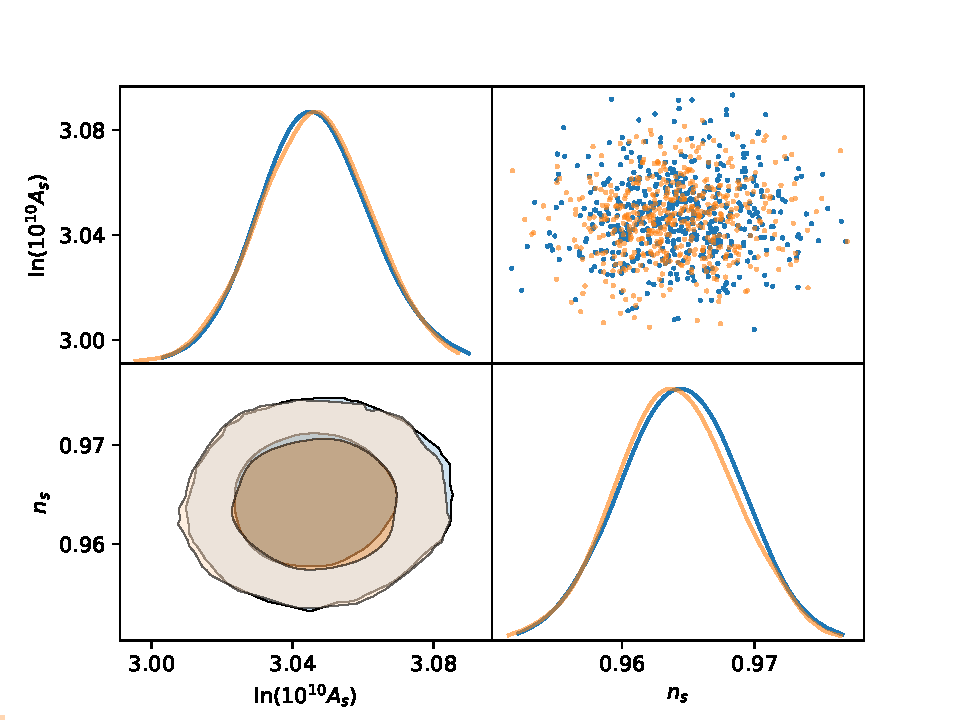
\includegraphics[width=0.5\textwidth]{./illustrations/misfit.pdf}
\caption{\label{org647915b}
An example of a posterior distribution generated with power posterior re-partitioning, based on data from planck. The posteriors are near identical, and a slight misfit can be explained with arithmetic rounding errors, and run-to-run variance of the position of the live points (see top right figure).}
\end{figure}




\subsection{Qualitative observations.}
\label{sec:orge463072}
Last but not least, an interactive cartoon of the convergence
process for as many parameters as one likes can be obtained from

\begin{verbatim}
NestedSamples().gui()
\end{verbatim}
This allows us to see how the points move during the execution of
nested sampling. A more crude picture can be obtained from the plot
of \(\ln Z\) vs \(\ln X\), (which is also present, and used as a
timeline).

Based on the typical shape of the curve, we shall distinguish the
following stages of the algorithm's convergence. 

While \(\ln Z \approx 0\), nested sampling is in its \emph{prior
compression} stage.  Afterwards the algorithm undergoes \emph{discovery}
where most live points enter the typical set and their number is
permanently reduced. The last stage is the \emph{extinction stage},
colloquially referred to as the \emph{tail}.


\subsection{Simulations}
\label{sec:orgc010171}
\subsubsection{Toy models}
\label{sec:orgc2eb631}

We shall begin our analysis with help of a simplified model that is
general-enough to share features with the Cosmological scale
problem, but also practical to investigate in depth, with multiple
variations.

Our original model is a Gaussian peak. By choosing the uniform
prior as a baseline, and setting the log-likelihood as:
\begin{equation}
  \ln {\cal L}(\theta) = - \frac{1}{2} \left\{(\theta - \mu)^{T}G^{-1}(\theta-\mu)  + \ln \det \left| 2\pi G\right| \right\}
\end{equation}
where the covariance matrix \(G\), specifies the extent of the peak,
and the vector \(\mu\), its location. We thus expect the posterior
to be a truncated and re-scaled Gaussian. However its typical set
is still approximately at a distance of the square root of the
diagonal elements of the covariance matrix form the peak, which we
shall refer to as \emph{one standard deviation}.

The covariance matrix is positive semi-definite and symmetric,
hence it can be diagonalised \citep{taboga2017lectures}. If the
covariance matrix is diagonal, the Gaussian distribution is called
uncorrelated. If all diagonal elements are equal, then the
Gaussian is spherical with characteristic diameter given by \(2
	\sigma = 2\sqrt{G}\), where \(G = G \mathds{1}\).

Notice that in this description we have completely neglected any
notion of ``data'', consequently, we don't need to worry about
generating said data, and the extra overheads associated with
\(\chi^2\) fitting.

Under such circumstances it's a matter of integrating \ref{eq:def-z}
to obtain the evidence. Most generally for a correlated Gaussian
likelihood the volume associated is 

\begin{equation}\label{eq:evidence}
   {\cal Z} = \frac{\left( \sqrt{ \det \left| 2\pi G \right|} \right)^{n}}{\mathbf{b}-\mathbf{a}}  
\end{equation}
where \(n\) is the number of parameters in the model.

The internal implementations of all our repartitioning schemes
contain two gaussians: one for the likelihood, and one
entering the repartitioning scheme to improve run-time. These
would be different in general and our simulations will reflect
that in the following ways.

The easiest to account for are translational offsets. One only needs to
modify the values of \(\theta' = \theta - \Delta\) entering \(\ln
	\mathcal{L}(\theta')\). 

One can, without loss of generality assume that one of the
Gaussians is uncorrelated (also WLOG, it's spherical);
effectively we need to apply a coordinate transformation
defined by the eigenvectors of the covariance matrix. We
cannot however assume that both are uncorrelated, nor that the
orthonormal vectors defining the Gaussian are aligned with the
boundaries of the uniform prior. Fortunately, these
complications contribute little. As we shall see, any
repartitioning scheme is easily able to cope with crude
approximations of the orientation and shape of the peak, and
run-time is affected negligibly. Consequently, outside of one
experiment, we shall ignore any deviations from a spherical
Gaussian.


\subsubsection{{\bfseries\sffamily TODO} Discuss tails.}
\label{sec:orga8d2fa9}
\subsubsection{{\bfseries\sffamily TODO} Cosmological simulations}
\label{sec:orgcc8c1c9}
For the Cosmological parameter estimation Cobaya \citep{cobaya} with
CLASS \citep{Blas_2011}, and PolyChord \citep{polychord} as a sampler
were chosen. The main reason being the high modularity of the code,
which allows a neater implementation of the re-partitioning
mac
\section{Results}
\label{sec:org31ac3de}
The first test case is an uncorrelated spherical Gaussian posterior
in three dimensions \(\mathcal{P}(\theta) = G(\theta; \mu = (1,2,3),
  \sigma = 1)\). The corresponding evidence (\autoref{eq:evidence}) is
\(\mathcal{Z}\approx-62.3\). First we shall assume that the mean and
standard deviation of all the repartitioning schemes is exactly the
same as that of the posterior. 

All but one re-partitioning scheme yielded the correct
evidence. The resizeable uniform prior model was constructed to
systematically overestimating the evidence (\autoref{fig:hist}),
which is due to underestimating the normalisation factor for
\(\mathcal{L}\).\footnote{the boundary dependence was omitted.}




\subsection{additive mixtures}
\label{sec:org52855a9}

Having proven the correctness of the runs, let's turn to
performance and benchmarks. The central metric is the number of
evaluations of \(\ln \mathcal{L}\). As we can see in
\autoref{fig:benchmark}, the fastest by far is the true posterior
distribution. Although it is difficult to see on the figure, the
number of evaluations is \(O(n_\text{live})\). 

On the same figure, we can also see confirmation of that the number
of \(\ln \mathcal{L}\) evaluations, is proportional to
\(n_\text{live}\). Crucially, one can see that the faster
repartitioning schemes also scale better. 

Of the repartitioning schemes, using the posterior directly, as our
intuition suggests, produces the best time, closely followed by the
stochastic mixture of it and the uniform reference. PPR, in the
case of exact coincidence of the mean and the standard deviation
produces a respectable speed-up. 

\begin{figure}
  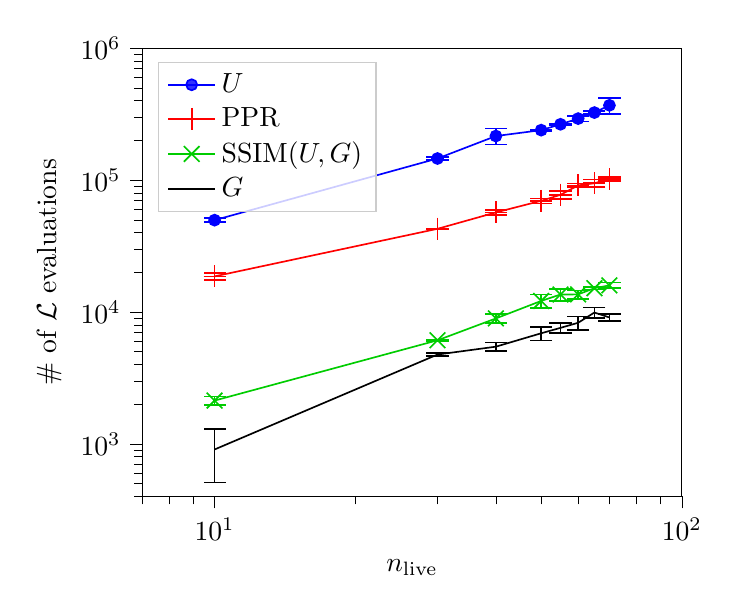
\begin{tikzpicture}

\definecolor{color0}{rgb}{0.0,0.0,1.0} %U
\definecolor{color1}{rgb}{1,0.0,0.0} %PPR
\definecolor{color2}{rgb}{0,0.8,0.0}                              %SSIM
\definecolor{color3}{rgb}{0.,0.0,0.0} %G

\begin{axis}[
legend cell align={left},
legend style={fill opacity=0.8, draw opacity=1, text opacity=1, at={(0.03,0.97)}, anchor=north west, draw=white!80!black},
tick align=outside,
tick pos=left,
x grid style={white!69.0196078431373!black},
xlabel={\(n_\text{live}\)},
xmin=7, xmax=100,
xtick style={color=black},
y grid style={white!69.0196078431373!black},
ylabel={\# of \({\cal L}\) evaluations},
ymin=400, ymax=1000000.0,
ytick style={color=black},
xmode=log,
ymode=log
]
\path [draw=color0, semithick]
(axis cs:10,48051.1762746562)
--(axis cs:10,51361.4903920105);

\path [draw=color0, semithick]
(axis cs:30,141787.579248368)
--(axis cs:30,149701.087418299);

\path [draw=color0, semithick]
(axis cs:40,185671.527674282)
--(axis cs:40,245784.472325718);

\path [draw=color0, semithick]
(axis cs:50,236296.832694899)
--(axis cs:50,241822.500638435);

\path [draw=color0, semithick]
(axis cs:55,262655.71356965)
--(axis cs:55,266952.953097016);

\path [draw=color0, semithick]
(axis cs:60,278243.015081106)
--(axis cs:60,306644.984918894);

\path [draw=color0, semithick]
(axis cs:65,317116.521541605)
--(axis cs:65,332736.145125062);

\path [draw=color0, semithick]
(axis cs:70,318358.948415036)
--(axis cs:70,419081.71825163);

\path [draw=color1, semithick]
(axis cs:10,17520.6487596482)
--(axis cs:10,19742.0179070185);

\path [draw=color1, semithick]
(axis cs:30,42472.9620658463)
--(axis cs:30,42994.371267487);

\path [draw=color1, semithick]
(axis cs:40,54281.6999405287)
--(axis cs:40,59494.3000594713);

\path [draw=color1, semithick]
(axis cs:50,66559.0160569084)
--(axis cs:50,72717.6506097582);

\path [draw=color1, semithick]
(axis cs:55,71552.6011973656)
--(axis cs:55,83118.7321359677);

\path [draw=color1, semithick]
(axis cs:60,88312.8386239607)
--(axis cs:60,94072.4947093726);

\path [draw=color1, semithick]
(axis cs:65,88215.9096228476)
--(axis cs:65,100992.090377152);

\path [draw=color1, semithick]
(axis cs:70,97882.04633)
--(axis cs:70,105637.95367);

\path [draw=color2, semithick]
(axis cs:10,1980.99743591911)
--(axis cs:10,2284.33589741422);

\path [draw=color2, semithick]
(axis cs:30,6035.87692136486)
--(axis cs:30,6174.12307863514);

\path [draw=color2, semithick]
(axis cs:40,8260.41435100755)
--(axis cs:40,9624.91898232578);

\path [draw=color2, semithick]
(axis cs:50,10733.0849396109)
--(axis cs:50,13538.9150603891);

\path [draw=color2, semithick]
(axis cs:55,12122.9645002052)
--(axis cs:55,15015.0354997948);

\path [draw=color2, semithick]
(axis cs:60,12622.7721075812)
--(axis cs:60,14593.2278924188);

\path [draw=color2, semithick]
(axis cs:65,14804.9685728395)
--(axis cs:65,15505.0314271605);

\path [draw=color2, semithick]
(axis cs:70,15158.1193669152)
--(axis cs:70,16693.8806330848);

\path [draw=color3, semithick]
(axis cs:10,511.628293172651)
--(axis cs:10,1305.03837349402);

\path [draw=color3, semithick]
(axis cs:30,4625.34584399058)
--(axis cs:30,4900.65415600942);

\path [draw=color3, semithick]
(axis cs:40,5045.39013421616)
--(axis cs:40,5880.60986578384);

\path [draw=color3, semithick]
(axis cs:50,6085.69651897324)
--(axis cs:50,7719.6368143601);

\path [draw=color3, semithick]
(axis cs:55,6959.0338647499)
--(axis cs:55,8215.63280191676);

\path [draw=color3, semithick]
(axis cs:60,7317.2571539732)
--(axis cs:60,9267.40951269347);

\path [draw=color3, semithick]
(axis cs:65,8986.02980736454)
--(axis cs:65,10838.6368593021);

\path [draw=color3, semithick]
(axis cs:70,8588.48027282128)
--(axis cs:70,9612.18639384539);


\addplot [semithick, color1, mark=-, mark size=4, mark options={solid}, only marks, forget plot]
table {%
10 17520.6487596482
30 42472.9620658463
40 54281.6999405287
50 66559.0160569084
55 71552.6011973656
60 88312.8386239607
65 88215.9096228476
70 97882.04633
};
\addplot [semithick, color1, mark=-, mark size=4, mark options={solid}, only marks, forget plot]
table {%
10 19742.0179070185
30 42994.371267487
40 59494.3000594713
50 72717.6506097582
55 83118.7321359677
60 94072.4947093726
65 100992.090377152
70 105637.95367
};
\addplot [semithick, color2, mark=-, mark size=4, mark options={solid}, only marks, forget plot]
table {%
10 1980.99743591911
30 6035.87692136486
40 8260.41435100755
50 10733.0849396109
55 12122.9645002052
60 12622.7721075812
65 14804.9685728395
70 15158.1193669152
};
\addplot [semithick, color2, mark=-, mark size=4, mark options={solid}, only marks, forget plot]
table {%
10 2284.33589741422
30 6174.12307863514
40 9624.91898232578
50 13538.9150603891
55 15015.0354997948
60 14593.2278924188
65 15505.0314271605
70 16693.8806330848
};
\addplot [semithick, color3, mark=-, mark size=4, mark options={solid}, only marks, forget plot]
table {%
10 511.628293172651
30 4625.34584399058
40 5045.39013421616
50 6085.69651897324
55 6959.0338647499
60 7317.2571539732
65 8986.02980736454
70 8588.48027282128
};
\addplot [semithick, color3, mark=-, mark size=4, mark options={solid}, only marks, forget plot]
table {%
10 1305.03837349402
30 4900.65415600942
40 5880.60986578384
50 7719.6368143601
55 8215.63280191676
60 9267.40951269347
65 10838.6368593021
70 9612.18639384539
};
\addplot [semithick, color0, mark=-, mark size=4, mark options={solid}, only marks, forget plot]
table {%
10 48051.1762746562
30 141787.579248368
40 185671.527674282
50 236296.832694899
55 262655.71356965
60 278243.015081106
65 317116.521541605
70 318358.948415036
};
\addplot [semithick, color0, mark=-, mark size=4, mark options={solid}, only marks, forget plot]
table {%
10 51361.4903920105
30 149701.087418299
40 245784.472325718
50 241822.500638435
55 266952.953097016
60 306644.984918894
65 332736.145125062
70 419081.71825163
};
\addplot [semithick, color0, mark=*, mark size=2, mark options={solid}]
table {%
10 49706.3333333333
30 145744.333333333
40 215728
50 239059.666666667
55 264804.333333333
60 292444
65 324926.333333333
70 368720.333333333
};
\addlegendentry{$U$}
\addplot [semithick, color1, mark=+, mark size=4, mark options={solid}]
table {%
10 18631.3333333333
30 42733.6666666667
40 56888
50 69638.3333333333
55 77335.6666666667
60 91192.6666666667
65 94604
70 101760
};
\addlegendentry{PPR}
\addplot [semithick, color2, mark=x, mark size=4, mark options={solid}]
table {%
10 2132.66666666667
30 6105
40 8942.66666666667
50 12136
55 13569
60 13608
65 15155
70 15926
};
\addlegendentry{$\text{SSIM}(U,G)$}
\addplot [semithick, color3, mark=., mark size=2, mark options={solid}]
table {%
10 908.333333333333
30 4763
40 5463
50 6902.66666666667
55 7587.33333333333
60 8292.33333333333
65 9912.33333333333
70 9100.33333333333
};
\addlegendentry{$G$}
\end{axis}

\end{tikzpicture}

\caption{\label{org15789e0}
comparison of likelihood calls necessary for obtaining the correct evidence for the case of a spherical uncorrelated Gaussian posterior. Note that almost all series scale linearly with the number of live points.}
\end{figure}




The next trial involves a variable offset, where convergence to the
correct posterior and evidence is not guaranteed even with the
correct normalisation.    

For this case, we have taken a Gaussian in a box of
\(1000\times1000\times1000\), and generated two nested sampling data
ranges. The ``offset'' posteriors are moved relative to the mean of
the prior. The parameter labeled '1' is offset by double the amount
of parameter '0'. 

The exemplary results are given in \autoref{fig:convergence}.

The main notable feature is the inaccuracy of the posterior for
power posterior repartitioning. One does expect it to produce the
correct posterior distribution if the offset is large compared to
the width of the peaks. If the offset is \(O(2\sigma)\), the
posterior is merely shifted, but if the shift is larger,
e.g. \(O(4\sigma)\), two peaks can be resolved. Unfortunately for
PPR, the evidence was also computed incorrectly: \(\ln {\cal
  Z}\approx -25.4 \pm 0.2\), vs the reference \(\ln {\cal Z} = -22.7 \pm
  0.4\).  Making matters even worse, the smaller of the two peaks is
actually the correct posterior.

This is the fatal flaw of PPR, that prevents it from being useful in
any real application. The constant, ever present bias implicit to
using a Gaussian prior causes the sampler to be strongly biased
towards the original value. It can be redeemed: the mixture model in
the same figure involves the same PPR as one of two models. It
produced the correct result, while also, remarkably managing to do
so faster than a uniform prior would allow\footnote{another method could
involve a prior on \(\beta\), that strongly favours values close to
\(\beta=0\).}.

\begin{figure}
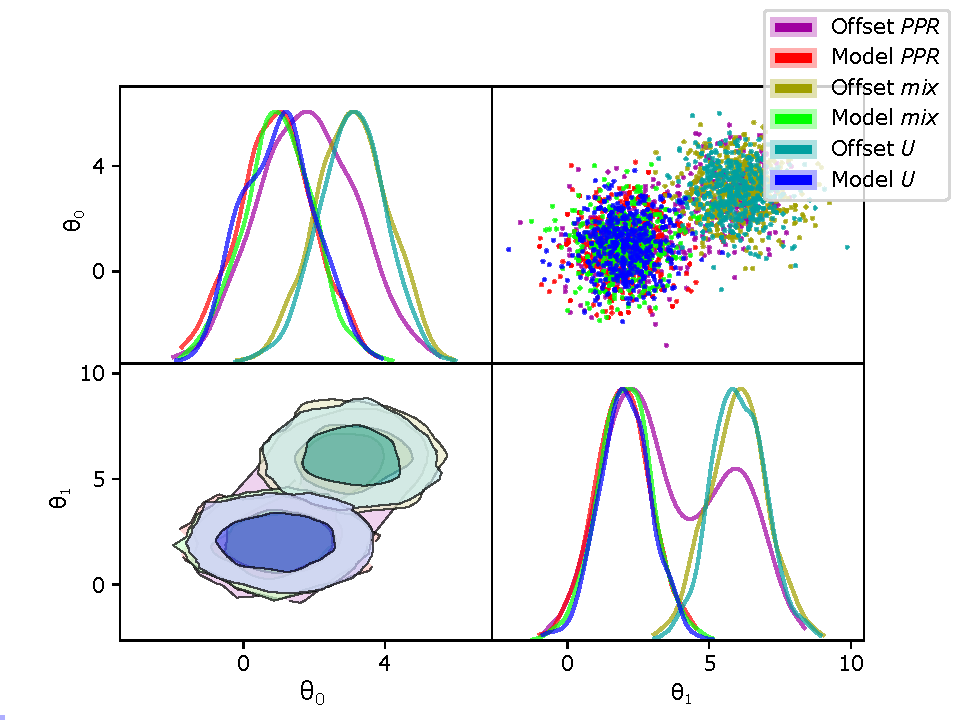
\includegraphics[width=0.5\textwidth]{./illustrations/convergence.pdf}
\caption{\label{orgbc72313}
An illustration of how offsets affect the convergence of nested sampling under different kinds of repartitioning. The offset models should produce an offset posterior, whilst sharing the prior with the model runs. The mixture is of the present uniform model and PPR.}
\end{figure}



\section{Discussion}
\label{sec:org91eeefc}
\section{Conclusions}
\label{sec:orge139b18}

\subsection{Results}
\label{sec:org4d264a3}
Our project's purpose had been to investigate the performance
increase attainable by algorithmic optimisations of the inputs to
nested samplers. 

We have identified a general prescription, named superpositional
mixture re-partitioning that netted the same if not greater
performance improvement as power posterior re-partitioning (PPR). 

We have also established that the aforementioned prescription had a
number of advantages:
\begin{itemize}
\item it allows multiple priors to be mixed, while PPR only allows one.
\item it permits a broader class of functions, than are practical for
PPR, e.g. ones where \(Z_{\pi}(\beta)\) cannot be represented in
closed form.
\item it copes with functions having different domains. PPR cannot.
\item it is abstract, i.e. the prior iCDF is a superposition iCDFs of
the constituents priors. For PPR the iCDF needs to be computed.
\item it supports an unbiased reference (uniform) prior exactly. PPR
tends to an unbiased reference as \(\beta\rightarrow\beta_{0}\).
\item TODO it is able to mitigate improper re-scaling of the
likelihood. If one of the priors is improperly normalised, the
offset from the true evidence is reduced as
\(n_{live}\rightarrow\infty\). PPR does not.
\item it is resilient to human error.
\item it is easier to implement and requires little to no mathematical
input from the user, beyond ensuring the three properties.
\end{itemize}


\subsection{Further research}
\label{sec:orgd642aaa}
The proposed algorithm of superpositional mixtures, maps neatly
onto concepts of quantum computation. Indeed one can model two
different priors as states of qubits. The benefits are potentially
immeasureable, as the greatest weakness of the classical algorithm
is that we're effectively sacrificing resolution in the posterior
by sampling only from one prior exclusively. Quantum superposition
allows us to do both at the same time, while quantum entanglement
ensures that the deterministic requirements set by
\citeauthor{skilling2006} are met.

The necessary consequence of repartitioning is that the posterior
samples have a greater prior space to explore, and thus, while the
option to skip areas of negligible evidence allows us to compress
the priors significantly more quickly, the tail-end of the nested
sampling is also affected. A potential solution to this is to treat
the introduced parameters separately at this stage.

One such treatment may be to use the posterior distribution at the
point of discovery to freeze the choice parameters. Their
covariance may represent a volume in a \(\theta\) space that
corresponds to the remaining evidence, and as such, crudely
approximate the remainder while sampling from a lower dimensional
space compounding to the physical (i.e. not re-partitioning-related
parameters of the theory).

Additionally, we have assumed that nested sampling converges the
fastest if the prior is also the posterior. However, a simple
example of a spherical Gaussian in three dimensions shows the same
characteristic tail at the end of the execution. It may be
necessary to look into priors that are tailor made to accelerate
that convergence. Naturally, they would also depend on the sampling
technique used: the prior that accelerates rejection sampling would
be different to one that accelerates slice sampling.

An additional avenue to explore would be to ask whether the same
sampling tecnhique is appropriate for all stages. Slice sampling is
ideal for applications with prior space with large
dimensions. However, Metropolis-Hastings may be more suitable for
the extinction phase, and may thus eliminate the tail altogether.

Among the less-important investigations that could be carried out,
one might investigate an extension of the re-sizeable uniform
prior. Indeed one of the main reasons for its impracticality is the
sharp reduction to zero, that cannot be compensated for in the
likelihood. However, one should expect that this is possible to
compensate for by using a distribution that's constructed to be
non-zero in the entire domain of the original uniform prior:
e.g. by having edges that tend to zero at the boundaries. A
suggestion might be a smooth top-hat, or a combination of error
functions.

\subsection{Applications}
\label{sec:orgc367a34}
Nested sampling is a universal algorithm that can be applied to any
problem involving either direct parameter estimation (e.g. analysis
of Planck data), or indirectly such as neural-network based machine
learning.

To clarify the latter point, the process of training a neural
network involves a process of estimating the connection strengths
between layers of states. Normally training is done via a negative
feedbakc process, where the connections that correspond to the
right answer are reinforced, whilst connections leading to
incorrect ones are reduced in strength. In the formalism of
Bayesian inference, the connection strenghts are the parameters,
the prior is uniform and the sampling is done via
Metropolis-Hastings anticipating a logistical distribution. As we
are able to accelerate this process in Bayesian formalism, we
should also be able to modify the standard algorithms to make use
of repartitioning.

Moreover, the subject matter of this paper superpositional mixture
repartitioning with stochastic sampling can be used to create
classes of neural networks: as of now information obtained from
training one network cannot be re-used when training another,
unless the two networks have identical architecture and solve
identical problems. One cannot use the weights of a network
analysing faces as the initial values for analysing objects,
without that resulting in a strong bias. 

It may be possible to use the values of node connection strengths
from networks that are used for similar problems, by virtue of the
stability offered by repartitioning. We can regard that as one of
the priors in the mixture, and hence improving performance where
the guess is indeed accurate, without compromising the result if it
is not. Of course such neural networks will need to have a similar
number of physical connections, and hence have similar if not
identical architecture.

\bibliography{bibliography} 
\bibliographystyle{mnras}

\section{Appendices}
\label{sec:org37cf61f}

\subsection{Why do we need to alter the likelihood.}
\label{sec:orgf73448c}
One may ask why such a change of the likelihood is at all
necessary. Indeed, the likelihood may be chosen based on a precise
theory of error, e.g. a least-squares fit argument based on
Gaussian assumptions. Why does changing the prior knowledge
necessitate the change of likelihood?

In addition to what was mentioned in answer to a similar question
at the end of the previous subsection, there's an intuitive way of
answering this question. Consider a posterior distribution that at
no point takes the value nil (e.g. a Gaussian).]. If we constrain one
prior \(\pi\) to lie within one standard deviation of the peak,
(e.g. a sphere of radius \(\sigma\)), and another that spans twenty
standard deviations. If we picked 20 points at random from one and
the other, we shall expect that the iso-likelihood hyper-surfaces
would encase drastically different volumes. Moreover, finding a
point that's within one standard deviation from the perspective of
the broader prior is a much more significant result than finding
one from the narrower one. Indeed, we will not expect the posterior
distributions to be the same, but nested sampling would produce a
narrower peak based on the ``same'' model\footnote{from a frequentist's point of view, our prior knowledge is
irrelevant. But even a frequentist would agree that the value obtained
by changing the prior would not be the same.}. 

Of course, a Bayesian would say that if our true prior knowledge
was represented by the narrower prior, we would indeed need to
consider the posterior distribution to be the true one, as it
combines information that we've obtained earlier with information
that can be extracted from the data. In other words, it would be
the correct value for the person who indeed constrained the values
of model parameters to the one standard deviation, based on \emph{other
data}. Simply picking a prior out of thin air would bias the
result, hence the necessity to repartition. 



\subsection{Obtaining a prior inversion function from the closed form of}
\label{sec:org564ddab}
\end{document}